\documentclass[a4paper,12pt,dutch]{article}
\usepackage{glossaries}
\usepackage[T1]{fontenc}
\usepackage{babel}
\usepackage{graphicx}
\usepackage[table,xcdraw]{xcolor}
\usepackage{hyperref}
\usepackage{blindtext}
\usepackage{geometry}
\usepackage{parskip}
\usepackage{mathtools}
\usepackage{siunitx}
\usepackage{listings}
\usepackage{csquotes}
\usepackage{caption}
\usepackage{subcaption}
\usepackage{comment}
\usepackage{pdfpages}
\usepackage[useregional]{datetime2}
\usepackage{amsmath} % for the equation* environment
\usepackage{float}
\usepackage{pict2e}
\usepackage{fixltx2e}
\usepackage{tocloft}
\usepackage{graphicx}
\usepackage{xcolor}
\usepackage{float}

%%gmedina solution
\newcommand{\listequationsname}{Lijst van berekeningen}
\newlistof{myequations}{equ}{\listequationsname}
\newcommand{\myequations}[1]{%
\addcontentsline{equ}{myequations}{\protect\numberline{\theequation}#1}\par}
\setlength{\cftmyequationsnumwidth}{2.5em}% Width of equation number in List of Equations

\DeclareRobustCommand{\slashcirc}{{\mathpalette\doslashcirc\relax}}

\makeatletter
\newcommand\doslashcirc[2]{%
  \sbox\z@{$#1\m@th\circ$}%
  \setlength\unitlength{\wd\z@}
  \begin{picture}(1,1)
  \roundcap
  \put(0,0){\box\z@}
  \put(0,0){\line(1,1){1}}
  \end{picture}%
}
\makeatother


% %% Some packages you will need
% \usepackage{pgfplots}
% \usepackage{pgfplotstable}
% \usepackage{booktabs}
% \usepackage{array}
% \usepackage{colortbl}


\definecolor{arduinoorange}{HTML}{FFA500}
\definecolor{arduinogray}{HTML}{808080}
\definecolor{arduinoblue}{HTML}{007ACC}
\definecolor{arduinogreen}{HTML}{469B00}

\lstset{
  language=C++,
  basicstyle=\ttfamily\footnotesize,
  keywordstyle=\color{arduinoorange},
  stringstyle=\color{arduinogreen},
  commentstyle=\color{arduinogray},
  moredelim=[s][\color{arduinoblue}]{\#}{\ },
  morekeywords={digitalRead,digitalWrite,pinMode,analogRead,analogWrite,Serial,begin,HIGH,LOW},
  frame=tb,
  tabsize=4,
  showstringspaces=false,
  breaklines=true,
  numbers=left,
  numberstyle=\tiny\color{arduinogray},
  numbersep=5pt,
  extendedchars=true,
  literate={á}{{\'a}}1 {ã}{{\~a}}1 {é}{{\'e}}1,
}

\lstdefinestyle{Arduino}
{
  language=C++,
  basicstyle=\ttfamily\footnotesize,
  keywordstyle=\color{arduinoorange},
  stringstyle=\color{arduinogreen},
  commentstyle=\color{arduinogray},
  moredelim=[s][\color{arduinoblue}]{\#}{\ },
  morekeywords={digitalRead,digitalWrite,pinMode,analogRead,analogWrite,Serial,begin},
  frame=tb,
  tabsize=4,
  showstringspaces=false,
  breaklines=true,
  numbers=left,
  numberstyle=\tiny\color{arduinogray},
  numbersep=5pt,
  extendedchars=true,
  literate={á}{{\'a}}1 {ã}{{\~a}}1 {é}{{\'e}}1,
  backgroundcolor=\color{black!85},
  rulecolor=\color{arduinoorange},
  frame=single,
  frameround=tttt,
  framexleftmargin=6pt,
  framexrightmargin=6pt,
  framextopmargin=6pt,
  framexbottommargin=6pt,
  breaklines=true,
  postbreak=\raisebox{0ex}[0ex][0ex]{\ensuremath{\color{red}\hookrightarrow\space}},
}

\usepackage[
    backend=biber,
    backref=true,
    backrefstyle=none,
    sortcites=true,
    sorting=none,
    doi=false, % doi informatie wordt niet weergegeven
    %uniquename=true,
    %uniquelist=true,
    maxcitenames=3,
    %issn=false, werkt niet
    language=american
]{biblatex}
\addbibresource{information/Bronnen.bib}
\DefineBibliographyStrings{dutch}{
    backrefpage = {blz.},
    backrefpages = {blz.},
}
\makeglossaries
\definecolor{Grey1}{HTML}{343434}
\graphicspath{{./Media/Figuren/}}
 \geometry{
 a4paper,
 total={170mm,257mm},
 left=20mm,
 top=20mm,
 }
\hypersetup{
    colorlinks=true,
    linkcolor=blue,
    filecolor=magenta,      
    urlcolor=cyan,
    pdftitle={Overleaf Example},
    pdfpagemode=FullScreen,
    }


\begin{document}
\title{

\includegraphics[width=3.5in]{IMG/logo/finalcircle.png} \\
\vspace*{1in}
\textbf{Project 3}\\
\textit{PVA Duurzame Energie}\\
Versie 1
}
\author{
\vspace*{1in} \\
  Geschreven door:\\
  Laurens van der Drift\\
  Tommy Dobos\\
		\vspace*{0.2in} \\
		De Haagse Hogeschool\\
        \textbf{Elektrotechniek}\\
        Delft, Nederland
       } 
\maketitle
%\addcontentsline{toc}{section}{Verklarende Woordenlijst}
\printglossaries
\newglossaryentry{tender}
{
    name=\textit{tender},
    description={De inschrijving om op een kavel een wind turbine park te bouwen.}
}
\newglossaryentry{energie akkoord}
{
    name=\textit{energie akkoord},
    description={Het Energieakkoord vertegenwoordigt duurzame groei, met betrokkenheid van 40+ organisaties waaronder overheid, werkgevers en milieuactivisten. Het bevat afspraken over energiebesparing, schonere technologie en klimaatbeleid.}
}
\newglossaryentry{offshore}
{
    name=\textit{offshore},
    description={Op enige afstand van de kust.}
}
\newglossaryentry{subsidie}
{
    name=\textit{subsidie},
    description={Een financiële bijdrage die je kunt krijgen van een overheids- of een particuliere organisatie.}
}
\newglossaryentry{joint venture}
{
    name=\textit{joint venture},
    description={Een joint venture (gezamenlijke onderneming) is een afspraak tussen bestaande bedrijven om samen te werken.}
}
\newglossaryentry{natuurinclusief}
{
    name=\textit{natuurinclusief},
    description={Natuurinclusief bouwen betekent dat er bewust ruimte voor biodiversiteit wordt gecreëerd op, aan of in het gebouw of de (openbare) omgeving, zodat er meer diverse planten- en diersoorten kunnen leven.}
}
\phantomsection
\addcontentsline{toc}{section}{Lijst van figuren}
\listoffigures
\newpage
\tableofcontents
\section{Voorwoord}
Cleaneco is een bedrijf ontstaan in augustus 2023 te Delft en is opgericht door Laurens van der Drift en Tommy Dobos.

Ingenieurs- en consultancybureau Worley heeft het ontwerp bedrijf Cleaneco aangenomen om een offshore windpark te ontwerpen op kavel VI en VII van Hollandse Kust West en hiervoor de tender te schrijven voor Rijkswaterstaat. 

De reden voor de aanleg van het windturbinepark op zee is hoofdstuk 4.2.2 van het energie akkoord\cite{energieakkoord} van 6 september 2013. In dit akkoord is afgesproken dat in 2023, 4450MW aan windvermogen op zee opgewekt moet worden. Met als doel genoeg vermogen opwekken voor vijf miljoen huishoudens. 

\section{Samenvatting}
\subsection{Project naam}
Voor dit project, Project Windpark Op Zee is het bedrijf Cleaneco in dienst genomen door Worley. 

\subsection{Probleem}
De Nederlandse overheid moet voldoen aan het \gls{energie akkoord}\cite{energieakkoord}, dat is vastgelegd op 6 september 2013. Dit akkoord stelt dat tegen 2023 een uitbreiding van het operationeel windvermogen op zee moet zijn gerealiseerd van 3450 MW. De al bestaande parken wekken ongeveer 1000 MW op. Samen zal dit dus ongeveer 4450 MW aan windvermogen moeten worden.

% De Nederlandse overheid moet voldoen aan het \gls{energie akkoord} vastgelegd op 6 september 2013.
% Hierin staat aangegeven dat in 2023 een opschaling moet hebben plaatsgevonden voor een operationeel windvermogen op zee van 4450MW. De reeds bestaande parken en hetgeen reeds in de pijplijn zit, tellen op tot circa 1000MW.
% Hoe kan de Nederlandse overheid de groei van windenergie op zee naar 4450 MW operationeel vermogen in 2023 bevorderen, met focus op kostenreductie, technologische vooruitgang, ruimtelijke planning en het overwinnen van belemmeringen, om zo aan de eisen te voldoen van het \gls{energie akkoord} opgesteld in september 2023?

\subsection{Doelstelling en Resultaat}
Onder opdracht van Worley is het aan Cleaneco om een technisch ontwerp te maken van een windturbinepark op zee. Hiervoor moet ook een onderhoudsplan worden opgesteld voor de komende 25 jaar. Het technisch ontwerp en onderhoudsplan zullen in de vorm van een adviesrapport aan de opdrachtgever gepresenteerd worden.

Uiterlijk in 2023 wordt een operationeel windvermogen van 4450 MW op zee gerealiseerd, in overeenkomst met de eisen van het \gls{energie akkoord}\cite{energieakkoord} van september 2013. Dit wordt bereikt met meetbare kostenverlaging, technologische vooruitgang, doelgerichte ruimtelijke planning en het succesvol aanpakken van belemmeringen. Dit project heeft significante maatschappelijke relevantie, het draagt namelijk bij aan de verduurzaming van de energieopwekking. Naast de naar schatting vijf miljoen\cite{energieakkoord} huishoudens die zullen profiteren van de duurzame energievoorziening, zal dit project bijdragen aan het vergroten van de kennis en ervaring op het front van windparken op zee.  

\subsection{Eisen} \label{Eisen}
Er moet aan de volgende eisen worden voldaan:
\begin{itemize}
   \item Er moet onderzoek gedaan worden naar nodige producten/materialen zoals: windturbines, kabels en transformator boxen. Hierbij moeten de energieopbrengsten voor twee verschillende turbines worden onderzocht.
   \item Er moeten twee verschillende ontwerpen komen voor de positionering van de windturbines. 
   \item Er moet een operationeel windvermogen op zee van 4450MW opgeleverd worden.
   \item Er moet een onderhoudsplan meegeleverd worden voor de komende 25 jaar.
   % \item Alles moet in een adviesrapport aan de opdrachtgever Worley gepresenteerd worden. 
   \item Alles moet in een adviesrapport gepresenteerd worden aan de opdrachtgever Worley.
 \end{itemize}

\subsection{Probleem oplossing}
Cleaneco zal een ontwerprapport en onderhoudsplan leveren aan Worley. Het rapport beantwoordt de \gls{tender} voor het \gls{offshore} windturbinepark. Het onderhoudsplan waarborgt dat het \gls{offshore} windpark op zee 25 jaar operationeel is. Bij projectvoltooiing volgt een adviesrapport. Om dit te realiseren zal onderzoek gedaan worden naar de punten genoemd onder hoofdstuk \ref{Eisen}. 

Het type onderzoek zal vallen onder het zogenoemde, bronnenonderzoek. De bronnen zullen onder andere komen van de database van de Haagse Hogeschool en professionals in het betreffende vakgebied.

\section{Kosten en Opbrengsten}
    \subsection{Financiële kosten en budget}
    Bouwkosten Windpark: Hoewel specifieke bouwkosten niet worden vermeld in de verstrekte informatie, kan worden aangenomen dat de bouw van een windpark van 756 MW met 54 windturbines aanzienlijke kapitaalinvesteringen met zich meebrengt. Dit omvat de kosten voor het ontwerpen, fabriceren en installeren van de windturbines en de benodigde infrastructuur op zee.

    Milieueffectrapportages en Locatiestudies: Er wordt vermeld dat Ecowende kosten draagt voor milieueffectrapportages en locatiestudies. Deze studies zijn nodig om de impact van het windpark op het milieu en de omgeving te beoordelen en te minimaliseren.

    Overheidsinkomsten: De overheid ontvangt € 63,5 miljoen van de partijen als gevolg van financiële biedingen en bijdragen van Ecowende. Dit geld wordt gebruikt om nieuwe windparken beter te integreren in de omgeving en voor overige activiteiten op de Noordzee.

    % \subsection{Verklarende woordenlijst}
Tijdslijn van het Project:

    2022: Ecowende, een \gls{joint venture} van Shell en Eneco, wint de vergunning voor het windpark Hollandse Kust (west) kavel VI.

    2023: Ontwerp en plannen worden gemaakt, en de bouw van het windpark is gepland om te beginnen in dit jaar.

    2026: Het windpark wordt naar verwachting volledig operationeel en levert elektriciteit.

Het maken van het windturbineparkontwerp en het onderhoudsplan zal gebeuren in een periode van 17 weken. Hiervan zal aan het begin ongeveer 60\% van de tijd besteed worden aan het maken van het windparkontwerp, de overige tijd zal worden gestoken in het realiseren van het onderhoudsplan en het verwerken van beide producten in het adviesrapport.\cite{studiewijzer} 

\subsection{Opbrengsten}

    Duurzame Energievoorziening: Het windpark Hollandse Kust (west) zal naar verwachting een vermogen van 756 MW genereren. Dit komt overeen met ongeveer 3\% van de Nederlandse elektriciteitsvraag, wat voldoende is om ongeveer een miljoen huishoudens van elektriciteit te voorzien. De opbrengst voor eindgebruikers is een toename van duurzame energievoorziening en een verminderde afhankelijkheid van niet-hernieuwbare bronnen zoals fossiele brandstoffen.

    Milieubescherming: Het ontwerp van het windpark is '\gls{natuurinclusief}' en omvat maatregelen om de impact op de natuur en het milieu te minimaliseren. Dit omvat bijvoorbeeld het creëren van een gezond ecosysteem, het minimaliseren van de impact op vogels, het onderwaterleven, en het stimuleren van biodiversiteit onder water. De opbrengst hier is een stap in de richting van milieubescherming en behoud van biodiversiteit.

    Toekomstige Groene Energie: Het windpark maakt deel uit van de groeiende inspanningen om groene energie in Nederland te vergroten. Dit draagt bij aan de ambitie om tegen 2030 ongeveer 21 GW aan windenergie op zee te hebben, wat een duurzame energiebron voor de toekomst zal opleveren.

    Economische Impuls: De bouw van windparken op zee kan een economische impuls geven aan de regio, met potentiële werkgelegenheidskansen in havens zoals Vlissingen, IJmuiden, Den Helder en de Eemshaven.

Samengevat, het project levert duurzame energie, milieubescherming, toekomstige groene energiebronnen en economische kansen op voor de eindgebruikers en de samenleving als geheel.\cite{Windenergiegebied}\cite{ShellEneco}\cite{Windopzee}

% % Opbrengst:

% % https://www.noordzeeloket.nl/functies-gebruik/windenergie/doorvaart-medegebruik/hollandse-kust-west/

% % https://www.rvo.nl/onderwerpen/bureau-energieprojecten/afgesloten-projecten/woz-hollandse-kust-west-kavels-vi-vii

% % https://www.rijksoverheid.nl/actueel/nieuws/2022/12/15/shell-en-eneco-winnen-tender-windpark-op-zee-hollandse-kust-west
\subsection{Plan van Aanpak}
Het eerste product dat geleverd zal worden is het plan van aanpak. In het plan van aanpak staan alle plannen en belangrijke informatie voor het opzetten van het project. Dit document zal worden geleverd voordat aan het project begonnen wordt. Daarnaast zal het ook gepresenteerd worden in een korte pitch van twee minuten. Het doel van het plan van aanpak is, het creëren van duidelijkheid over: de verwachtingen van de opdrachtgever, de doelen waar naartoe moet worden gewerkt en hoe, en de belangrijke informatie over het project, zoals mogelijke risico's, te ondernemen acties en de werkwijze. 

\subsection{Parkontwerp}
Het tweede product dat gemaakt en geleverd zal moeten worden is het parkontwerp. Het windturbinepark staat in dit project centraal, hiervan zal dan ook een uitgewerkt ontwerp worden geleverd. Hierin worden technische aspecten behandeld, zo zullen twee type windturbines worden uitgewerkt, voor beide zal ook de optimale positionering worden bepaald voor de beste opbrengst. Dit zal bepaald worden door het gedrag van de wind op de kavels te analyseren. Er zal ook worden ingegaan op de verwachte energieopbrengsten voor de gekozen turbines. 

Bij het parkontwerp hoort natuurlijk ook een uitwerking van de bekabeling, de specificaties van de kabels zelf, en de uitwerking van de onderlinge connecties en die met het hoogspanningsstation. Bij het ontwerpen van het windturbinepark zal ook rekening worden gehouden met het effect dat alle hiervoor genoemde elementen zullen hebben op de onderhoud van het park. 

\subsection{Onderhoudsplan}
Het derde product dat geleverd zal worden is het onderhoudsplan. In het onderhoudsplan zal komen welke componenten, met welke frequentie, onderhoud nodig zullen hebben. Ook wordt ingegaan op de soort onderhoud en hoe dit moet gebeuren. De frequentie zal worden gebaseerd op en onderbouwd door statistische gegevens over de verschillende componenten van windturbineparken. Met de frequentie zal vervolgens een onderhoudsstrategie gemaakt worden dat ook verwerkt wordt in het onderhoudsplan. 

Verder zal er in het onderhoudsplan worden besproken hoe de conditie van de componenten bewaakt zal worden. Ten slotte zullen de risico's van het plegen van onderhoud worden uitgewerkt in het plan. 

\subsection{Adviesrapport}
Als laatste product zal het adviesrapport worden opgesteld voor Worley. In het adviesrapport zullen de belangrijkste aspecten van de vorige producten worden samengevat. Zo zal de probleemstelling van het project aan bod komen samen met de gekozen turbine types en verwachte energieopbrengsten. Verder zal het parkontwerp inclusief bekabeling en de bijbehorende kabelberekeningen in het adviesrapport worden verwerkt. Ten slotte zal ook het onderhoudsplan niet uit het adviesrapport worden weggelaten. Ter afsluiting van het project zal dit adviesrapport (aan Worley) worden gepresenteerd. 

\section{Programma van eisen}
\subsection{Plan van Aanpak}
Het eerste product dat geleverd zal worden is het plan van aanpak. In het plan van aanpak staan alle plannen en belangrijke informatie voor het opzetten van het project. Dit document zal worden geleverd voordat aan het project begonnen wordt. Daarnaast zal het ook gepresenteerd worden in een korte pitch van twee minuten. Het doel van het plan van aanpak is, het creëren van duidelijkheid over: de verwachtingen van de opdrachtgever, de doelen waar naartoe moet worden gewerkt en hoe, en de belangrijke informatie over het project, zoals mogelijke risico's, te ondernemen acties en de werkwijze. 

\subsection{Parkontwerp}
Het tweede product dat gemaakt en geleverd zal moeten worden is het parkontwerp. Het windturbinepark staat in dit project centraal, hiervan zal dan ook een uitgewerkt ontwerp worden geleverd. Hierin worden technische aspecten behandeld, zo zullen twee type windturbines worden uitgewerkt, voor beide zal ook de optimale positionering worden bepaald voor de beste opbrengst. Dit zal bepaald worden door het gedrag van de wind op de kavels te analyseren. Er zal ook worden ingegaan op de verwachte energieopbrengsten voor de gekozen turbines. 

Bij het parkontwerp hoort natuurlijk ook een uitwerking van de bekabeling, de specificaties van de kabels zelf, en de uitwerking van de onderlinge connecties en die met het hoogspanningsstation. Bij het ontwerpen van het windturbinepark zal ook rekening worden gehouden met het effect dat alle hiervoor genoemde elementen zullen hebben op de onderhoud van het park. 

\subsection{Onderhoudsplan}
Het derde product dat geleverd zal worden is het onderhoudsplan. In het onderhoudsplan zal komen welke componenten, met welke frequentie, onderhoud nodig zullen hebben. Ook wordt ingegaan op de soort onderhoud en hoe dit moet gebeuren. De frequentie zal worden gebaseerd op en onderbouwd door statistische gegevens over de verschillende componenten van windturbineparken. Met de frequentie zal vervolgens een onderhoudsstrategie gemaakt worden dat ook verwerkt wordt in het onderhoudsplan. 

Verder zal er in het onderhoudsplan worden besproken hoe de conditie van de componenten bewaakt zal worden. Ten slotte zullen de risico's van het plegen van onderhoud worden uitgewerkt in het plan. 

\subsection{Adviesrapport}
Als laatste product zal het adviesrapport worden opgesteld voor Worley. In het adviesrapport zullen de belangrijkste aspecten van de vorige producten worden samengevat. Zo zal de probleemstelling van het project aan bod komen samen met de gekozen turbine types en verwachte energieopbrengsten. Verder zal het parkontwerp inclusief bekabeling en de bijbehorende kabelberekeningen in het adviesrapport worden verwerkt. Ten slotte zal ook het onderhoudsplan niet uit het adviesrapport worden weggelaten. Ter afsluiting van het project zal dit adviesrapport (aan Worley) worden gepresenteerd. 

% Onpersoonlijk:
\section{Wat zijn de belangrijke aspecten van de kavels VI en VII?} \label{Wat zijn de belangrijke aspecten van de Kavels VI en VII?}

Er zijn veel aspecten van de kavels VI en VII waar rekening mee moet worden gehouden. Enkele belangrijker dan anderen. Ten eerste is de locatie van de kavels van belang. De kavels maken onderdeel uit van het windenergiegebied Hollandse Kust west en liggen op ongeveer 53 km van de west kust van Nederland en heeft een oppervlakte van circa 176 km\textsuperscript{2}.\cite{SiteDescriptionRVO} De twee kavels zullen elk een \gls{offshore} windcapaciteit van 700MW realiseren.\cite{SiteDescriptionRVO}\cite{Functies&gebruikHKW}

Om het windpark te ontwerpen dat instaat is dit te bieden zijn verschillende andere data van de kavels belangrijk. Er moet bepaald worden wat de beste positionering is voor de windturbines. Bij de beslissing hiervan moeten aspecten in acht genomen worden, zoals al bestaande en geplande infrastructuur van pijpleidingen en kabels. Daarnaast moet rekening worden gehouden met potentiële wrakken, magnetische abnormaliteiten en oude boorgaten zoals genoteerd staat in Appendix C van de locatie beschrijving (zie figuur \ref{fig:obstakels}).\cite{SiteDescriptionRVO}\cite{AppendixC} Uit voorzorg zullen, de windturbines op een minimale afstand van 100 meter van de genoemde obstakels geplaatst worden. Dit zal echter pas later van toepassing zijn, aangezien er voorlopig nog geen parkindeling is gemaakt. 
\begin{figure}[h]
\centering
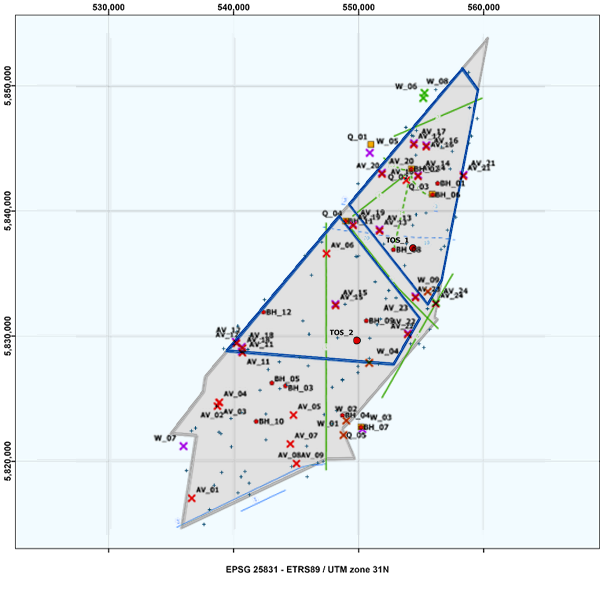
\includegraphics[width=0.5\textwidth]{IMG/data/overzicht/Map.png}
\caption{Gecombineerde map van obstakels.}
\label{fig:obstakels}
\end{figure}

Er is ook informatie over de kavels die significant is voor het besluit over de te kiezen windturbines en de oriëntatie hiervan. De informatie die hiervoor belangrijk is, is de winddata, zoals windsnelheden en -richtingen over langere periodes. Deze data is te halen uit de Wind Resource Assessment.\cite{WindResourceAssessment} In dit document staat winddata van metingen die zijn uitgevoerd over een periode van twee jaar, van 07-02-2019 tot 06-02-2021. Deze metingen zijn gedaan op een hoogte van 100 meter boven het gemiddelde zeeniveau en zijn dus representatief voor de te verwachten winden die de windturbines zullen ervaren. De statisch gemiddelde gemeten windsnelheid was over deze periode 10,06 m/s. 

Behalve de windsnelheid, is ook de windrichting van belang. De windrichting was net zoals de windsnelheid variërend, echter is er wel een overheersende windrichting bepaald. De overheersende windrichting is WZW (West-Zuid-West), deze windrichting kwam voor 21,2\% van de gemeten periode voor. De tweede meest significante windrichting was ZZW (Zuid-Zuid-West), met 20,1\%. 





% Er is naar een veelvoud windturbines gezocht en gekeken. Bekeken modellen waren onder andere de volgende:
% \begin{itemize}
%     \item De SG 14-236 DD, 14 MW windturbine van Siemens Gamesa.\cite{SiemensGamesa14MW}
%     \item De V236-15.0, 15 MW windturbine van Vestas.
%     \item De Haliade-X, 12 MW windturbine van GE renewable energy.\cite{GEHalideX}
%     \item 
% \end{itemize}

\section{Berekeningen}
\subsection{Algemene berekeningen}
\subsubsection{Swept Area}
Van de uitgekozen windturbines zijn meerdere gegevens verzameld, waaronder de diameter. Hiermee is het rotoroppervlakte (A(\(m^2\))) te berekenen zoals gedaan in formules \ref{eq:1} en \ref{eq:2}.
\begin{equation} \label{eq:1}
% \text{12MW Turbine geeft: } \pi*(\slashcirc/2)^2 = \pi*(222/2)^2 = 38707
\text{12MW Turbine geeft: } A =\pi*(\frac{\slashcirc_{12MW}}{2})^2 = \pi*(\frac{222}{2})^2 = 38707 m^2
\end{equation}
\myequations{Berekening: A 12MW Turbine}

\begin{equation} \label{eq:2}
\text{18MW Turbine geeft: } A =\pi*(\frac{\slashcirc_{18MW}}{2})^2 = \pi*(\frac{263}{2})^2 = 54325 m^2
\end{equation}
\myequations{Berekening: A 18MW Turbine}

De diameter van de twee turbines verschilt, vanwege de kwadratische berekening die gepaard gaat met het berekenen van de oppervlakte, is het effect hiervan groter terug te zien in het rotoroppervlak.
\subsubsection{Theoretisch vermogen}
Met het rotoroppervlak van de turbines is het theoretische vermogen dat uit de wind gehaald kan worden, te berekenen. Dit vermogen kan berekend worden met de formules \ref{eq:3} en \ref{eq:4} hieronder. 

\begin{equation} \label{eq:3}
    P_{wind12MW} = \frac{1}{2}*1.29*A_{12MW}*v_{wind}^3 = \frac{1}{2}*1.29*38707*v_{wind}^3
\end{equation}
\myequations{Berekening: Pwind 12MW Turbine}

\begin{equation} \label{eq:4}
    P_{wind18MW} = \frac{1}{2}*1.29*A_{18MW}*v_{wind}^3 = \frac{1}{2}*1.29*54325*v_{wind}^3
\end{equation}
\myequations{Berekening: Pwind 18MW Turbine}

\subsubsection{Tussenberekeningen}
De snelheid van de wind op de kavels is variërend, deze formules zijn dus toegepast voor realistische en te verwachten windsnelheden gebaseerd op de windgegevens over een periode van twee jaar.\cite{WindResourceAssessment} 
De uitkomsten zijn in een tabel genoteerd en geplot zoals te zien in (figuur \ref{fig:TVUW}). In realiteit is dit theoretische vermogen niet volledig uit de wind te halen, er is namelijk sprake van het Betzlimiet. 

\begin{figure}[H]
\centering
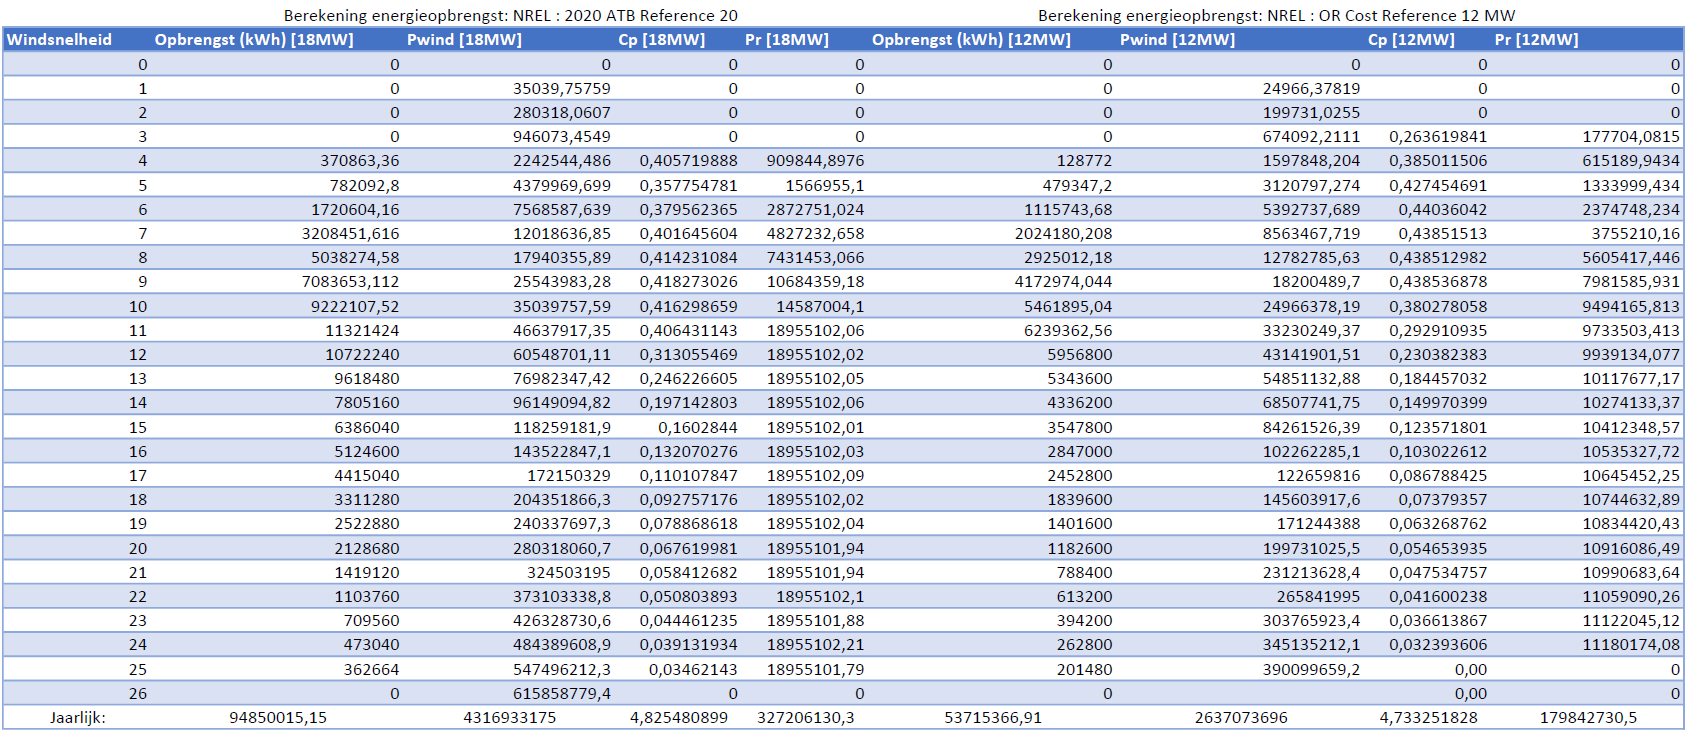
\includegraphics[width=1\textwidth]{IMG/data/overzicht/TVUW.PNG}
\caption{Gegevens: windsnelheid, energieopbrengst, vermogen en Cp}
\label{fig:TVUW}
\end{figure}

\subsubsection{Cp}
Elke windturbine heeft een vermogensfactor (Cp). Door het windvermogen te vermenigvuldigen met de Cp van de windturbine, wordt het werkelijk op te wekken vermogen verkregen. Ook de Cp is variabel, wat betekent dat het vermogen dat de turbine uit de wind kan halen ook zal verschillen afhankelijk van de windsnelheid. De plot van de Cp is te zien in (figuur \ref{fig:CpGraph}). De uitkomsten van de formules \ref{eq:5} en \ref{eq:6} zijn wederom genoteerd en geplot zoals te zien in (figuur \ref{fig:PrGraph}). 
\begin{figure}[H]
\centering
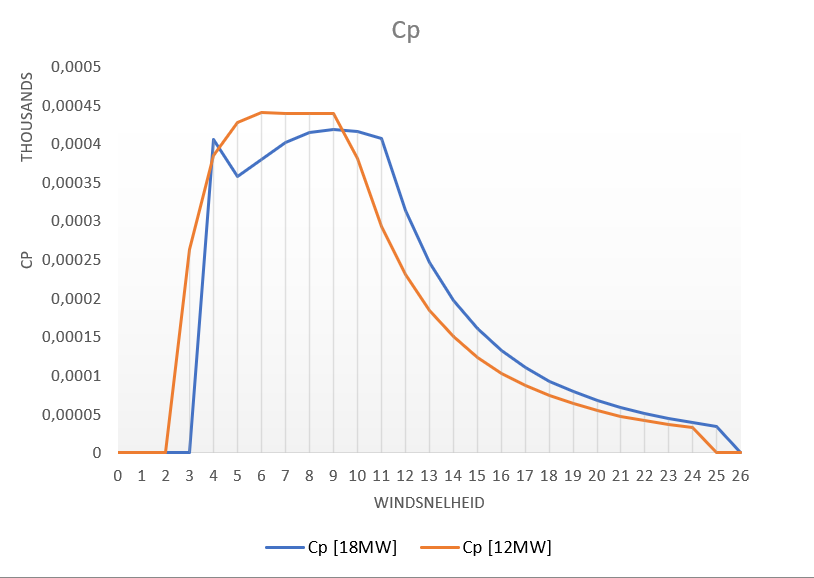
\includegraphics[width=0.7\textwidth]{IMG/data/overzicht/Cp_graph.PNG}
\caption{Plot: Cp\textsubscript{18MW} en Cp\textsubscript{12MW}}
\label{fig:CpGraph}
\end{figure}
\subsubsection{Pr}
\begin{figure}[H]
\centering
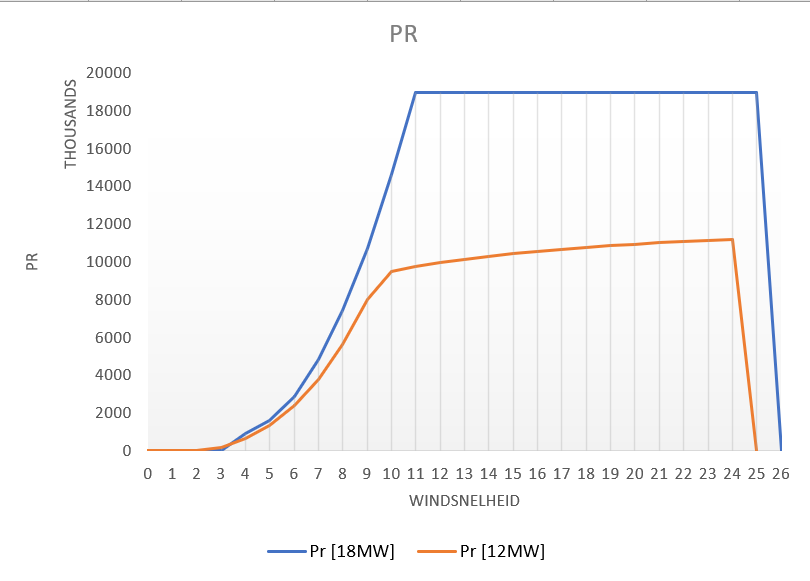
\includegraphics[width=0.7\textwidth]{IMG/data/overzicht/Pr_graph.PNG}
\caption{Plot: Pr\textsubscript{18MW} en Pr\textsubscript{12MW}}
\label{fig:PrGraph}
\end{figure}


\begin{equation} \label{eq:5}
\text{Werkelijk vermogen 12MW turbine: } P_{r12MW}=Cp_{12MW}*P_{wind12MW}
\end{equation}
\myequations{Berekening: Werkelijk vermogen 12MW turbine}

\begin{equation} \label{eq:6}
\text{Werkelijk vermogen 18MW turbine: } P_{r18MW}=Cp_{18MW}*P_{wind18MW}
\end{equation}
\myequations{Berekening: Werkelijk vermogen 18MW turbine}

\subsubsection{Wind data}
Uit de Wind Resource Assessment\cite{WindResourceAssessment} is de benodigde winddata gehaald. Hieronder valt ook informatie over de frequentie van gemeten windsnelheden gedurende een periode van twee jaar. Deze frequentie kan gebruikt worden als de kans op de windsnelheid. Met formule \ref{eq:7} kan berekend worden hoeveel uur een windsnelheid per jaar zal plaatsvinden als deze overeen komt met de bepaalde kans. In onderstaande formule (\ref{eq:7}) staat X voor de kans / het percentage dat de windsnelheid voorkomt in een jaar. 

\begin{equation} \label{eq:7}
\text{Frequentie windsnelheid in uren/jaar: } 365*24*X 
\end{equation}
\myequations{Berekening: Frequentie windsnelheid}


De verdeling van de frequentie van de windsnelheden over de span van de gemeten periode\cite{WindResourceAssessment} staat in (figuur \ref{fig:Frequentieverdeling}). 
\begin{figure}[H]
\centering
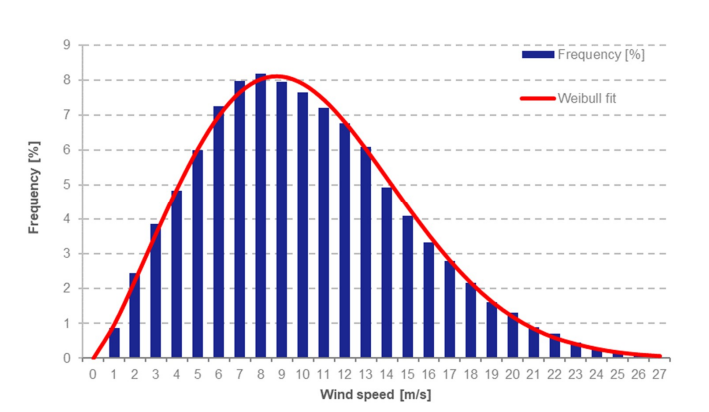
\includegraphics[width=0.7\textwidth]{IMG/data/overzicht/Frequentieverdelingwind.PNG}
\caption{Gegevens: frequentie wind snelheid per jaar.}
\label{fig:Frequentieverdeling}
\end{figure}

\subsubsection{Energieopbrengst exclusief parkeffect}
Door de verdeling van het aantal uur dat de windsnelheden voorkomen in een jaar en de berekende werkelijke vermogens van de windturbines te gebruiken, kan de jaarlijkse energieopbrengst worden berekend. Dit wordt gedaan met de volgende formules: 

\begin{equation} \label{eq:8}
\text{12MW Turbine: } E_{opbrengst,12MW}=t_{uren per jaar}*P_{r12MW}
\end{equation}
\myequations{Berekening: Energie Opbrengst 12MW Turbine}

\begin{equation} \label{eq:9}
\text{18MW Turbine: } E_{opbrengst,18MW}=t_{uren per jaar}*P_{r18MW}
\end{equation}
\myequations{Berekening: Energie Opbrengst 18MW Turbine}

De uitkomsten hiervan zijn in (tabel \ref{fig:Jaaropbrengst}) genoteerd. Nu kan de jaaropbrengst berekend worden voor beide turbines, door de uitkomsten van dezelfde turbine bij elkaar op te tellen. Hieruit is gekomen dat de jaaropbrengst met de 18MW turbine overeen komt met 94.850.015 kWh, en met de 12MW turbine overeen komt met 53.715.367 kWh. Dit verschil is behoorlijk en geeft duidelijk aan hoezo de 18MW windturbine veel voordeliger en aantrekkelijker is om te gebruiken. 
\begin{figure}[H]
\centering
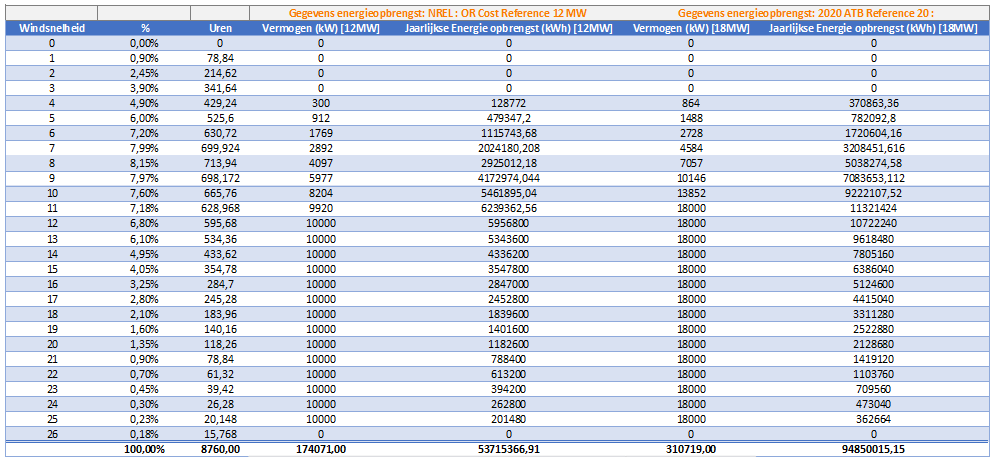
\includegraphics[width=1\textwidth]{IMG/data/overzicht/Jaaropbrengst.PNG}
\caption{Gegevens: Uren, Vermogens en Energieopbrengst.}
\label{fig:Jaaropbrengst}
\end{figure}
Bij deze jaarlijkse energieopbrengst is echter nog geen rekening gehouden met een aantal factoren die in de werkelijkheid een rol spelen, zoals het parkeffect. Om de jaarlijkse energieopbrengst inclusief het parkeffect te bepalen moet eerst het parkeffect berekend worden. Het parkeffect kan vervolgens vermenigvuldigd worden met de jaarlijkse energieopbrengst exclusief parkeffect, om de daadwerkelijke jaarlijkse energieopbrengst te krijgen. 

\subsubsection{Parkeffect}
Om dit parkeffect te berekenen, zijn een aantal tussenstappen gemaakt, waarbij verschillende berekeningen gemaakt zijn. De berekeningen moeten worden uitgevoerd voor beide kavels. Er is echter nog niet genoeg informatie gevonden over de oppervlaktes van de individuele kavels. Hier zal voor het volgende tussenrapportagemoment nog meer onderzoek naar gedaan worden. Voor nu is echter de oppervlakte van beide kavels bepaald door de oppervlakte van het windpark (176km\textsuperscript{2}) te delen door twee. Hierdoor is de oppervlakte voor beide kavels op het moment dus hetzelfde (88km\textsuperscript{2}), en verschilt er dus niks tussen de kavels. 

Om het parkeffect te berekenen zijn de volgende gegevens van belang: 
\begin{itemize}
    \item Aantal turbines per kavel
    \item Totale vermogen per kavel
    \item Oppervlakte kavel
    \item Vermogensdichtheid 
    \item Jaaropbrengst exclusief parkeffect
\end{itemize}

Ter vergelijking zijn deze berekeningen uitgevoerd voor beide windturbines. 

\subsection{Configuratie 1 (18MW)}
De eerste stap is het bepalen van het aantal turbines op de kavel. Volgens de eisen mag het totale rotoroppervlak niet groter zijn dan 2.624.613m\textsuperscript{2}, vanwege de grootte van het rotoroppervlak van de 18MW turbine, is de maximale hoeveelheid turbines die geplaatst kan worden volgens de eisen gelijk aan 48. 

De tweede stap is het totale vermogen op de kavel bepalen. Dit is het aantal turbines maal het vermogen per turbine, dus 48*18 = 864MW. Vervolgens moet de oppervlakte van het windpark bepaald worden. Hiervoor is, zoals eerder vermeld, dezelfde waarde genomen voor beide kavels, namelijk 88km\textsuperscript{2} wateroppervlak. 

Stap drie is het bepalen van de vermogensdichtheid. Om dit te berekenen kan de volgende formule gebruikt worden: 
\begin{equation} \label{eq:10}
\text{18MW Turbine: } P_{dichtheid18MW}=(\frac{n_{turbines}*P_{turbine}}{A_{oppervlak}}) = (\frac{48*18}{88}) = 9,818 MW/km\textsuperscript{2}
\end{equation}
\myequations{Berekening: P Dichtheid 18MW Turbine}

Vervolgens kan met de vermogensdichtheid het parkeffect berekend worden. Dit wordt gedaan met formule \ref{eq:11}. 

\begin{equation} \label{eq:11}
 Parkeffect_{18MW}=\frac{100-(\frac{n_{turbines}*P_{turbine}}{A})}{100} = \frac{100-P_{totaal}}{100}
\end{equation}
\myequations{Berekening: Parkeffect 18MW Turbine}

Het parkeffect varieert afhankelijk van de vermogensdichtheid. Deze is op zijn beurt weer afhankelijk van meerdere factoren. De berekende waardes van het parkeffect voor verschillende aantallen turbines staan in figuur \ref{fig:Parkeffect_table} is geplot in (figuur \ref{fig:ParkEffectGraph}). 

\begin{figure}[H]
\centering
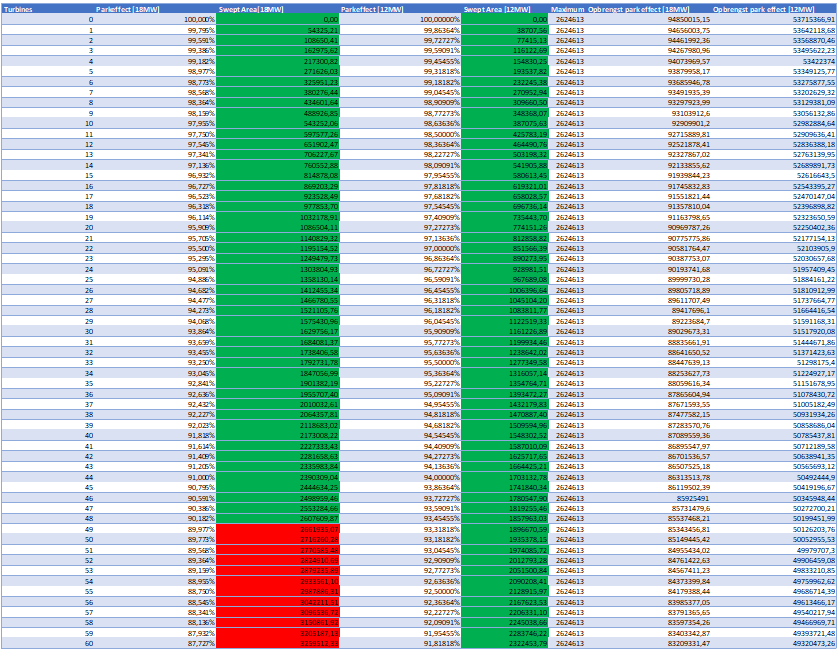
\includegraphics[width=1\textwidth]{IMG/data/overzicht/Parkeffect.PNG}
\caption{Gegevens: Aantal turbines, Parkeffect, Swept Area en Opbrengst park effect.}
\label{fig:Parkeffect_table}
\end{figure}

\begin{figure}[H]
\centering
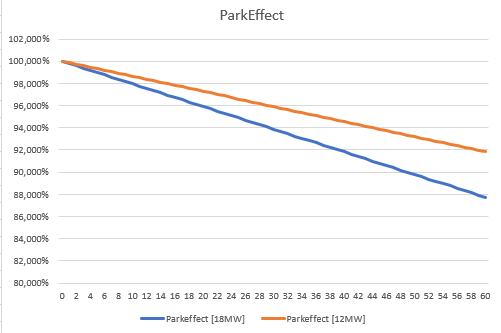
\includegraphics[width=0.7\textwidth]{IMG/data/overzicht/parkeffect_graph.PNG}
\caption{Plot: Parkeffect.}
\label{fig:ParkEffectGraph}
\end{figure}

Ten slotte kan met het parkeffect het daadwerklijke vermogen bepaald worden. Dit kan berekend worden door het parkeffect te berekenen voor het aantal turbines dat op de kavel komt. In dit geval gaat het om 48 turbines. Dus is het parkeffect: 

\begin{equation} \label{eq:12}
 Parkeffect_{18MW} = \frac{100-(P_{totaal}/A)}{100} = \frac{100-(864/88)}{100} = 0,902 = 90,2\%
\end{equation}
\myequations{Berekening: Parkeffect 18MW Turbine doorgerekend}

De jaarlijkse energieopbrengst inclusief het parkeffect is dan vrij simpel te berekenen met de formule: 
% \begin{equation} \label{eq:6}
% \text{Opbrengst 12MW kWh } t_{uren per jaar}*VermogenPerWindsnelheid_{12MW}
% \end{equation}
% \begin{equation} \label{eq:7}
% \text{Opbrengst 18MW kWh } t_{uren per jaar}*VermogenPerWindsnelheid_{18MW}
% \end{equation}


\begin{equation} \label{13}
\text{18MW Turbine: } OpbrengstParkeffect_{18MW}=Parkeffect_{18MW}*E_{opbrengst,18MW} 
\end{equation}
\myequations{Berekening: Opbrengst Parkeffect 18MW Turbine}

\begin{equation} \label{14}
OpbrengstParkeffect_{18MW}=0,902*94850015 = 85.554.713kWh 
\end{equation}
\myequations{Berekening: Opbrengst Parkeffect 18MW Turbine}

\subsection{Configuratie 2 (12MW)}
Voor configuratie 2 zijn de meeste berekeningen al uitgevoerd bij configuratie 1. Ook is het verschil duidelijk te zien in de figuren en is voor elke formule het alternatief gegeven voor de turbine van configuratie 2. 

De energieopbrengst inclusief parkeffect zal hieronder worden berekend voor de windturbine van 12MW. 

\begin{equation} \label{eq:15}
 Parkeffect_{12MW} = \frac{100-(P_{totaal}/A)}{100} = \frac{100-((60*12)/88)}{100} = 0,918 = 91,8\%
\end{equation}
\myequations{Berekening: Parkeffect 12MW Turbine doorgerekend}

\begin{equation} \label{eq:16}
OpbrengstParkeffect_{12MW}=Parkeffect_{12MW}*E_{opbrengst,12MW}
\end{equation}
\myequations{Berekening: Opbrengst Parkeffect 12MW Turbine}

\begin{equation} \label{eq:17}
OpbrengstParkeffect_{12MW}= 0,918*53715367 = 49.320.473 kWh
\end{equation}
\myequations{Berekening: Opbrengst Parkeffect 12MW Turbine}

Het verschil in jaarlijkse energieopbrengst, inclusief parkeffect, tussen de twee configuraties is dus 85.554.713 - 49.320.473 = 36.234.240 kWh aan energie per jaar. Dat is een zeer aanzienlijk getal. Dit is ook terug te zien in figuur \ref{fig:OpbrengstPark}

\begin{figure}[H]
\centering
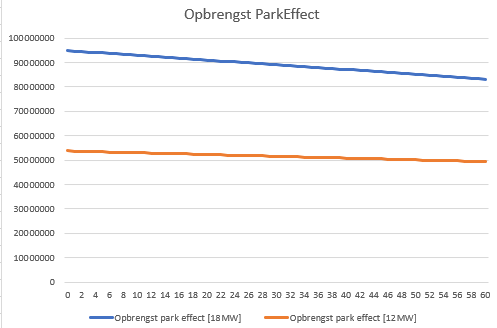
\includegraphics[width=0.7\textwidth]{IMG/data/overzicht/OpbrengstPark_graph.PNG}
\caption{Plot: OpbrengstPark.}
\label{fig:OpbrengstPark}
\end{figure}

% \section{Welke twee type windturbines zijn het meest geschikt voor het windpark en waarom?}
% Er zullen meerdere maatregelen worden genomen om de kwaliteit van de producten te waarborgen. Voor alle producten geldt dat er een eindredactie zal plaatsvinden. Bij de eindredactie zullen de documentaties worden gecontroleerd op inhoudelijke en verslagtechnische correctheid. Ook zullen voor alle producten alleen betrouwbare bronnen geraadpleegd worden met relevante informatie en actuele autoriteit. Daarnaast zal verwezen worden naar alle bronnen volgens de verslagtechnische eisen, met correcte toepassing van IEEE-richtlijnen. Verder zullen, ter verbetering van de leesbaarheid van het document, alle moeilijke termen genoteerd worden in een begrippenlijst.

% \subsection{Planning en taakverdelingen}
% Naast een eindredactie wordt, om de kwaliteit van de producten en de timing van de levering hiervan te garanderen, voor een goede organisatie gezorgd. Hieronder vallen een goede taakverdeling, planning en communicatie. Voor de taakverdeling en planning wordt het platform Github gebruikt, hierop zijn de taken per projectlid ingedeeld en ingepland. Zo kan worden verzekerd dat iedereen zich aan alle deadlines houdt. Als dit niet het geval blijkt te zijn, wordt dit besproken en zijn er consequenties. Naast Github is de planning ook in grote lijnen uitgewerkt in het plan van aanpak. 

% \subsection{Onderzoeksvragen}
% Met als doel het waarborgen van de structuur en kwaliteit van de documentaties, zal de probleemstelling worden opgedeeld in kleinere problemen. Deze problemen zullen worden uitgewerkt met behulp van onderzoeksvragen.\cite{projecthandleiding}
% De hoofdvraag voor het gehele project is: "\textbf{Hoe kunnen de eisen volgens het energieakkoord \cite{energieakkoord} van 2013 behaald worden met behulp van een windturbinepark op kavel VI en VII?}". De hoofdvraag zal worden beantwoord door middel van meerdere deelvragen. Voor tussenproduct 1, het park ontwerp, zullen de volgende vragen beantwoord worden\cite{projecthandleiding}:
% \begin{itemize}
%     \item Welke twee type windturbines zijn het meest geschikt voor het windpark en waarom?
%     \item Wat is de beste positionering van de windturbines voor optimale opbrengst, efficiënte bekabeling en makkelijker onderhoud?  
%     \item Welke kabels zijn geschikt voor het transporteren van de energie van turbines tot het hoogspanningsstation met de verwachte stromen?
%     \item Hoe ziet de bekabeling van het windpark eruit en waarom?
%     \item Wat  de beste soort spanning voor dit windturbinepark is, gelijk- of wisselspanning en welke effecten heeft dit op het park? %Bespreek transformator boxen
%     \item Welk invloed hebben de gemaakte keuzes op de onderhoud van het park? 
% \end{itemize}

% Ter beantwoording van tussenproduct 2, het onderhoudsplan, zijn de volgende deelvragen opgesteld:
% \begin{itemize}
%     \item Hoe wordt de conditie van de componenten waaruit het windturbinepark bestaat bewaakt? 
%     \item Welk onderhoud moet er plaatsvinden aan het windturbinepark?
%     \item Hoe frequent moet er onderhoud plaatsvinden en hoe is dit bepaald?
%     \item Hoe ziet de onderhoudsstrategie eruit? 
%     \item Welke materiële en financiële risico's zijn er bij het plegen van onderhoud?
% \end{itemize}

% Deze vragen uitgebreid beantwoorden garandeert dat alle belangrijke aspecten voor dit project behandeld worden. 

\section{Turbines}
\subsection{Introductie}
In de huidige wereld van hernieuwbare energie staan offshore windturbines als pion van een groenere toekomst. De keuze voor de juiste windturbine voor een project is cruciaal, en het verkrijgen van nauwkeurige en betrouwbare informatie over deze turbines is van het groot belang. Onderzoek heeft getoond dat er verscheidene turbines en fabrikanten zijn, waaronder de GE Haliade-X 14 MW, de Goldwind GWH252-16MW, de Vestas V236, de NREL 12MW en de NREL 18MW.
\subsection{GE Haliade-X 14 MW}
De GE Haliade-X 14 MW is een krachtige offshore windturbine met een aanzienlijk nominaal vermogen van 14 MW. Met een indrukwekkende rotordiameter van 220 meteren een jaarlijkse energieproductie van ongeveer 74 gigawattuur, speelt deze turbine een significante rol in de offshore windenergiesector. \cite{GEHalideX}\cite{TNOHalideX}\cite{TopsectorEnergieHalideX}\cite{OffshoreWindHalideX}\cite{AandrijftechniekHalideX}\cite{PonderaHalideX}
\subsection{Vestas V236}
De Vestas V236, met een vermogen van 15 MW en een rotordiameter van 236 meter, vertegenwoordigt eveneens een aanzienlijke keuze binnen de offshore windenergie sector. Desondanks wordt hij op het gebied van nominaal vermogen en jaarlijkse energieproductie overtroffen door de MySE-windturbine. \cite{Vestas15MW}\cite{Vestas}\cite{VestasJourney}\cite{WindTurbineModels}\cite{Electrek}\cite{OffshoreWindBiz3}
\subsection{Ming Yang MySE 16-260}
De MySE-windturbine, ontwikkeld door het Chinese bedrijf MingYang, heeft de aandacht getrokken vanwege zijn indrukwekkende technische specificaties en efficiëntie. Met een rotordiameter van 252 meter behoort deze windturbine tot de grootste in zijn categorie, wat hem in staat stelt om krachtige offshore winden effectief te benutten. Met een nominaal vermogen van 16 MW kan de MySE aanzienlijke hoeveelheden elektriciteit genereren, zelfs onder uitdagende omstandigheden.
Een opvallend kenmerk van de MySE-windturbine is zijn vermogen om windbronnen efficiënter te benutten dan sommige concurrenten. Dit wordt ondersteund door gegevens die aantonen dat de MySE vergelijkbare of zelfs grotere hoeveelheden elektriciteit kan produceren dan windturbines met een hoger nominaal vermogen.\cite{NewAtlas}\cite{MySEWebsite}\cite{OffshoreWindMySE}\cite{YouTube}\cite{MySEWebsite2}
\subsection{Goldwind GWH252-16MW}
De Goldwind GWH252-16MW, met een indrukwekkende rotordiameter van 252 meter, toont een opmerkelijke technologische prestatie. Echter, de beschikbare gegevens suggereren dat de MySE-windturbine van MingYang nog steeds vergelijkbare of zelfs grotere hoeveelheden elektriciteit kan genereren, wat impliceert dat de MySE mogelijk efficiënter is in het benutten van windenergiebronnen.\cite{Goldwind}\cite{4COffshore}
\subsection{National Renewable Energy Laboratory}
Na grondige overweging en uitgebreide vergelijkingen met deze concurrenten, is er besloten om de focus te richten op de windturbines van het National Renewable Energy Laboratory (NREL). En dat is om goede redenen.\cite{NRELVision}\cite{NRELAwards}
\subsubsection{NREL12MW}
De NREL 12MW Offshore windturbine, hoewel iets lager in vermogen dan zijn grotere broer, heeft ook indrukwekkende specificaties en prestaties. Met een rotordiameter van 222 meter en een geschatte jaarlijkse energieproductie van 12 gigawattuur, blijft deze windturbine een krachtige en efficiënte optie voor offshore windenergieprojecten.\cite{NRELOregonWindStudy}\cite{NRELATB2020}\cite{NRELReference12MW}\cite{NRELCsv12MW}

Specificaties van de NREL 12W Offshore windturbine:
\begin{itemize}
    \item \textbf{Naam:} NREL 12MW Offshore windturbine
    \item \textbf{Nominaal vermogen:} 12.000 kW
    \item \textbf{Geschatte windsnelheid:} 11 m/s
    \item \textbf{Aanvang windsnelheid:} 3 m/s
    \item \textbf{Stop windsnelheid:} 25 m/s
    \item \textbf{Rotordiameter:} 222 meter
    \item \textbf{Hubhoogte:} 136 meter
\end{itemize}


\subsubsection{NREL18MW}
Specificaties van de NREL 18MW Offshore windturbine:
\begin{itemize}
    \item \textbf{Naam:} NREL 18MW Offshore windturbine
    \item \textbf{Nominaal vermogen:} 18.000 kW
    \item \textbf{Geschatte windsnelheid:} 11 m/s
    \item \textbf{Aanvang windsnelheid:} 3 m/s
    \item \textbf{Stop windsnelheid:} 25 m/s
    \item \textbf{Rotordiameter:} 263 meter
    \item \textbf{Hubhoogte:} 150 meter
\end{itemize}

De NREL 18MW Offshore windturbine biedt enkele opmerkelijke voordelen die hem tot een uitstekende keuze maken. Met een nominaal vermogen van 18 MW, een indrukwekkende rotordiameter van 263 meter en een jaarlijkse energieproductie van maar liefst 80 gigawattuur, is deze windturbine een krachtige oplossing op zee. Zijn hoge capaciteitsfactor zorgt ervoor dat hij consistent een hoog rendement kan leveren en meer elektriciteit aan het net kan leveren.\cite{NRELReference18MW}\cite{NRELCSV18MW}\cite{NRELATB2020Specific}
\subsubsection{Vergelijking}
Bovendien bieden de NREL 18MW en NREL 12MW Offshore windturbines de geruststellende zekerheid van betrouwbare gegevens en informatie die online open source beschikbaar zijn. Om deze reden kan er een nauwkeurige berekeningen gemaakt worden en het project op de meest solide basis te bouwen.\cite{NRELTurbineModels}

De keuze voor de NREL 18MW en NREL 12MW Offshore windturbines is niet alleen gebaseerd op hun indrukwekkende technische specificaties, maar ook op de visie van het National Renewable Energy Laboratory om een schone energietoekomst voor de wereld te creëren. Hun inzet voor energiegerechtigheid en inclusieve ontwerpen sluit naadloos aan bij onze eigen waarden en doelen. \cite{NRELDiversity}\cite{NRELSustainability}\cite{NRELTurbineModels}
\subsection{Conclusie}
Terwijl de windturbines van MingYang, Goldwind en Vestas ongetwijfeld indrukwekkend zijn, hebben de NREL 18MW en NREL 12MW Offshore windturbines de overhand in termen van vermogen, efficiëntie en betrouwbare informatie. Het is een keuze die ons dichter bij een groenere, schonere toekomst brengt, waarin offshore windenergie een cruciale rol speelt in de transitie naar duurzame energiebronnen. Met de NREL 18MW en NREL 12MW Offshore windturbines aan onze zijde zijn we vastbesloten om een positieve impact te hebben op de wereld van hernieuwbare energie en een duurzamere planeet te creëren voor toekomstige generaties.
\section{Wat zijn de opbrengsten van het windpark?}
\subsection{Algemene berekeningen}
\subsubsection{Swept Area}
Van de uitgekozen windturbines zijn meerdere gegevens verzameld, waaronder de diameter. Hiermee is het rotoroppervlakte (A(\(m^2\))) te berekenen zoals gedaan in formules \ref{eq:1} en \ref{eq:2}.
\begin{equation} \label{eq:1}
% \text{12MW Turbine geeft: } \pi\times (\slashcirc/2)^2 = \pi\times (222/2)^2 = 38707
\text{12MW Turbine geeft: } A =\pi\times (\frac{\slashcirc_{12MW}}{2})^2 = \pi\times (\frac{222}{2})^2 = 38707 m^2
\end{equation}
\myequations{Berekening: A 12MW Turbine}

\begin{equation} \label{eq:2}
\text{18MW Turbine geeft: } A =\pi\times (\frac{\slashcirc_{18MW}}{2})^2 = \pi\times (\frac{263}{2})^2 = 54325 m^2
\end{equation}
\myequations{Berekening: A 18MW Turbine}

De diameter van de twee turbines verschilt, vanwege de kwadratische berekening die gepaard gaat met het berekenen van de oppervlakte, is het effect hiervan groter terug te zien in het rotoroppervlak.

\subsubsection{Theoretisch vermogen}
Met het rotoroppervlak van de turbines is het theoretische vermogen dat uit de wind gehaald kan worden, te berekenen. Dit vermogen kan berekend worden met de formules \ref{eq:3} en \ref{eq:4} hieronder. 

\begin{equation} \label{eq:3}
    P_{wind12MW} = \frac{1}{2}\times 1.29\times A_{12MW}\times v_{wind}^3 = \frac{1}{2}\times 1.29\times 38707\times v_{wind}^3
\end{equation}
\myequations{Berekening: Pwind 12MW Turbine}

\begin{equation} \label{eq:4}
    P_{wind18MW} = \frac{1}{2}\times 1.29\times A_{18MW}\times v_{wind}^3 = \frac{1}{2}\times 1.29\times 54325\times v_{wind}^3
\end{equation}
\myequations{Berekening: Pwind 18MW Turbine}

\subsubsection{Tussenberekeningen}
De snelheid van de wind op de kavels is variërend, deze formules zijn dus toegepast voor realistische en te verwachten windsnelheden gebaseerd op de windgegevens over een periode van twintig jaar.\cite{WindData}
De uitkomsten zijn in een tabel genoteerd en geplot zoals te zien in (figuur \ref{fig:TVUW}). In realiteit is dit theoretische vermogen niet volledig uit de wind te halen, er is namelijk sprake van het Betzlimiet.

\begin{figure}[H]
\centering
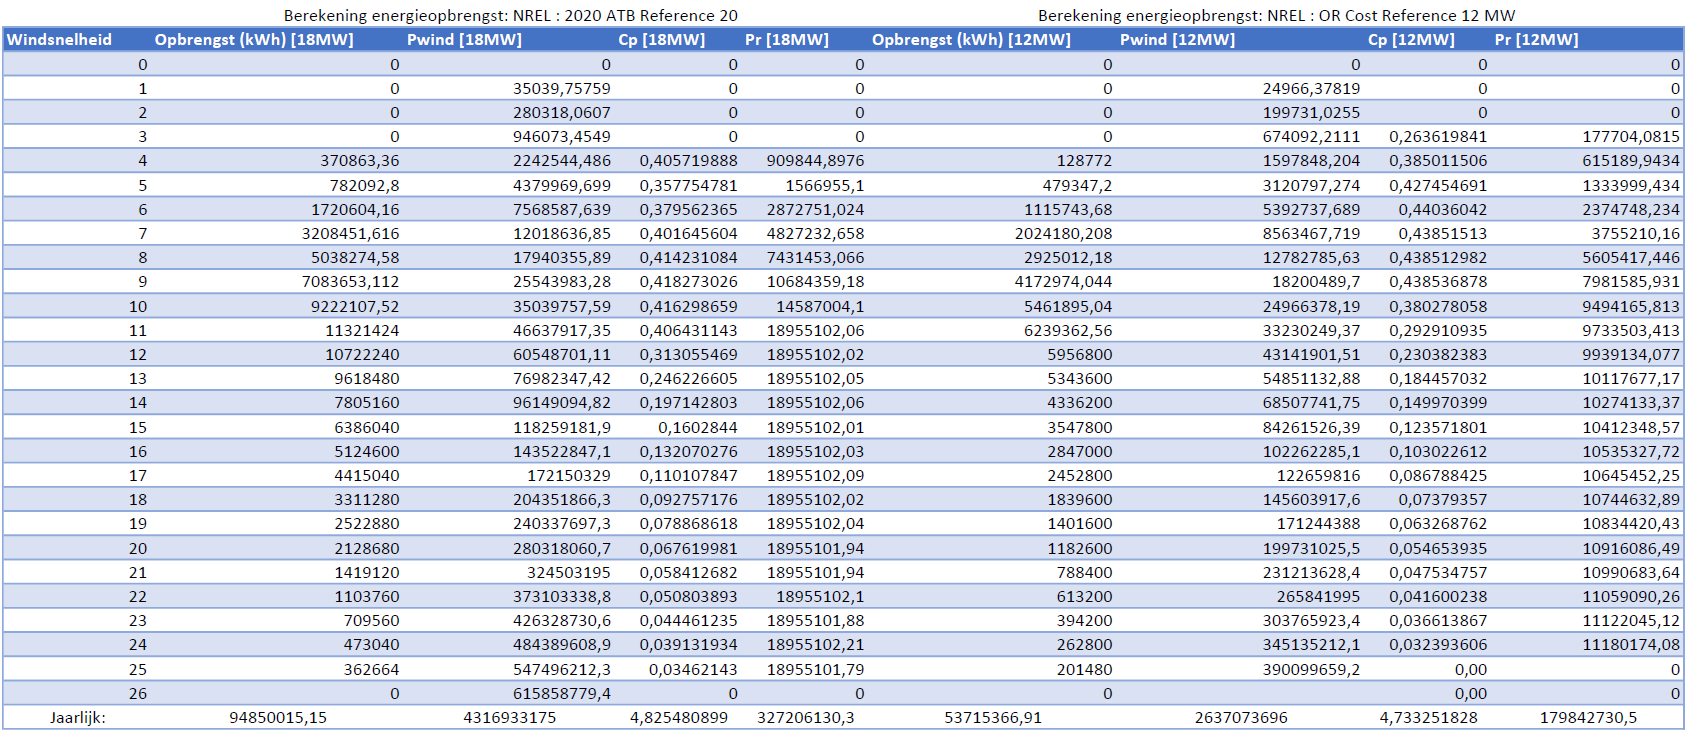
\includegraphics[width=1\textwidth]{IMG/data/overzicht/TVUW.PNG}
\caption{Gegevens: windsnelheid, energieopbrengst, vermogen en Cp}
\label{fig:TVUW}
\end{figure}

\subsubsection{Cp}
Elke windturbine heeft een vermogensfactor (Cp). Door het windvermogen te vermenigvuldigen met de Cp van de windturbine, wordt het werkelijk op te wekken vermogen verkregen. Ook de Cp is variabel, wat betekent dat het vermogen dat de turbine uit de wind kan halen ook zal verschillen afhankelijk van de windsnelheid. De plot van de Cp is te zien in (figuur \ref{fig:CpGraph}). De uitkomsten van de formules \ref{eq:5} en \ref{eq:6} zijn wederom genoteerd en geplot zoals te zien in (figuur \ref{fig:PrGraph}). 
\begin{figure}[H]
\centering
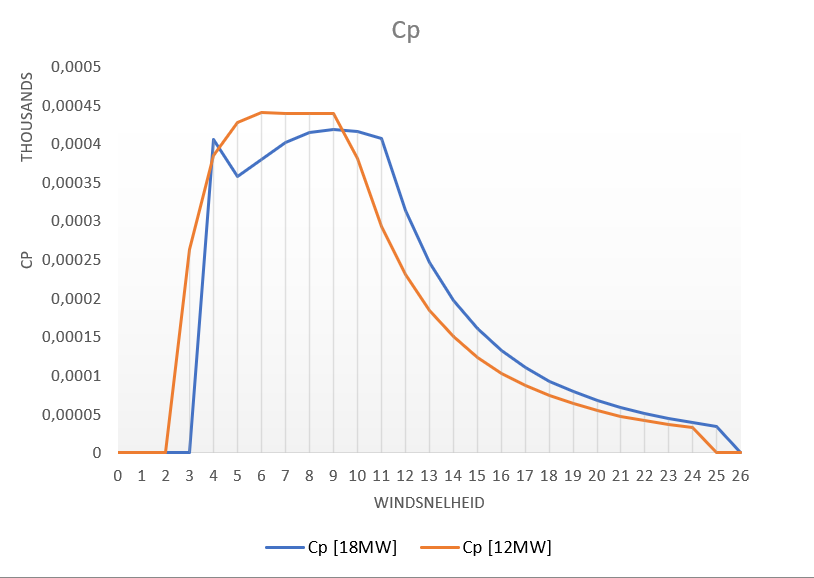
\includegraphics[width=0.7\textwidth]{IMG/data/overzicht/Cp_graph.PNG}
\caption{Plot: Cp\textsubscript{18MW} en Cp\textsubscript{12MW}}
\label{fig:CpGraph}
\end{figure}
\subsubsection{Pr}
\begin{figure}[H]
\centering
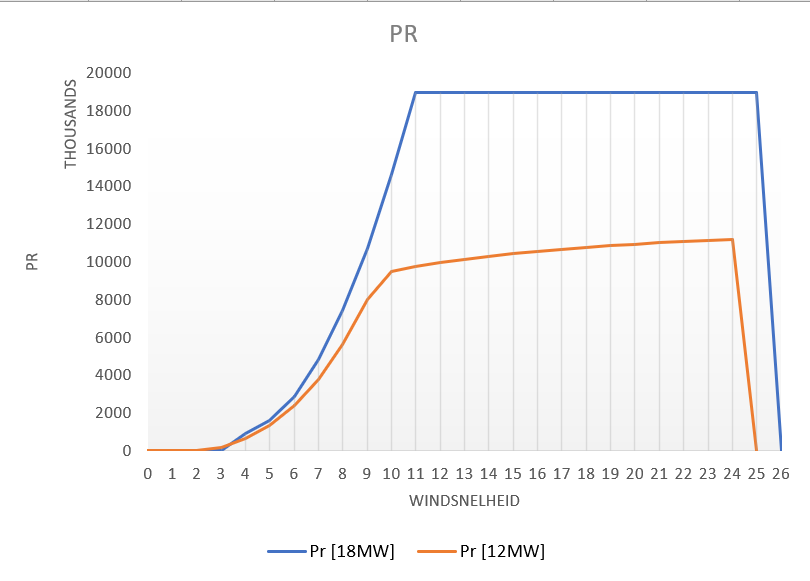
\includegraphics[width=0.7\textwidth]{IMG/data/overzicht/Pr_graph.PNG}
\caption{Plot: Pr\textsubscript{18MW} en Pr\textsubscript{12MW}}
\label{fig:PrGraph}
\end{figure}


\begin{equation} \label{eq:5}
\text{Werkelijk vermogen 12MW turbine: } P_{r12MW}=Cp_{12MW}\times P_{wind12MW}
\end{equation}
\myequations{Berekening: Werkelijk vermogen 12MW turbine}

\begin{equation} \label{eq:6}
\text{Werkelijk vermogen 18MW turbine: } P_{r18MW}=Cp_{18MW}\times P_{wind18MW}
\end{equation}
\myequations{Berekening: Werkelijk vermogen 18MW turbine}

\subsubsection{Energieopbrengst exclusief parkeffect}
Door de verdeling van het aantal uur dat de windsnelheden voorkomen in een jaar en de berekende werkelijke vermogens van de windturbines te gebruiken, kan de jaarlijkse energieopbrengst worden berekend. Dit wordt gedaan met de volgende formules: 

\begin{equation} \label{eq:8}
\text{12MW Turbine: } E_{opbrengst,12MW}=t_{uren per jaar}\times P_{r12MW}
\end{equation}
\myequations{Berekening: Energie Opbrengst 12MW Turbine}

\begin{equation} \label{eq:9}
\text{18MW Turbine: } E_{opbrengst,18MW}=t_{uren per jaar}\times P_{r18MW}
\end{equation}
\myequations{Berekening: Energie Opbrengst 18MW Turbine}

De uitkomsten hiervan zijn in (tabel \ref{fig:Jaaropbrengst}) genoteerd. Nu kan de jaaropbrengst berekend worden voor beide turbines, door de uitkomsten van dezelfde turbine bij elkaar op te tellen. Hieruit is gekomen dat de jaaropbrengst met de 18MW turbine overeen komt met 94.850.015 kWh, en met de 12MW turbine overeen komt met 53.715.367 kWh. Dit verschil is behoorlijk en geeft duidelijk aan hoezo de 18MW windturbine veel voordeliger en aantrekkelijker is om te gebruiken. 
\begin{figure}[H]
\centering
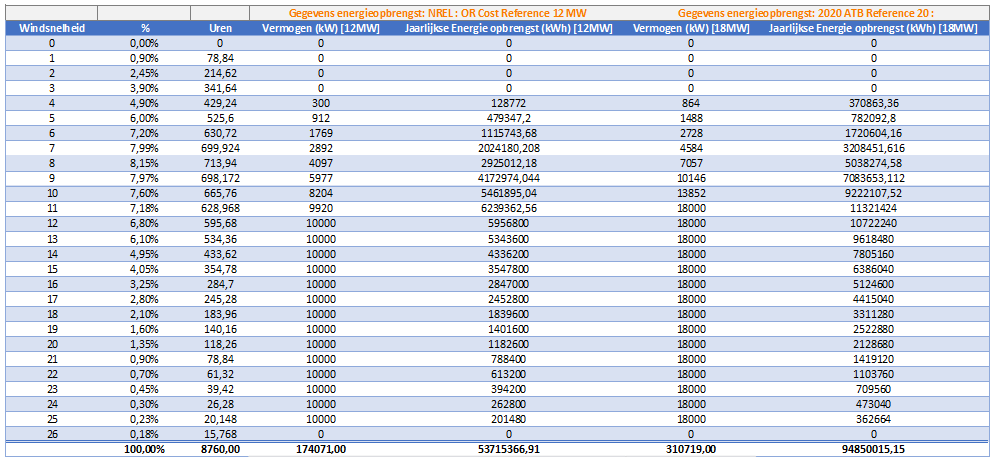
\includegraphics[width=1\textwidth]{IMG/data/overzicht/Jaaropbrengst.PNG}
\caption{Gegevens: Uren, Vermogens en Energieopbrengst.}
\label{fig:Jaaropbrengst}
\end{figure}
Bij deze jaarlijkse energieopbrengst is echter nog geen rekening gehouden met een aantal factoren die in de werkelijkheid een rol spelen, zoals het parkeffect. Om de jaarlijkse energieopbrengst inclusief het parkeffect te bepalen moet eerst het parkeffect berekend worden. Het parkeffect kan vervolgens vermenigvuldigd worden met de jaarlijkse energieopbrengst exclusief parkeffect, om de daadwerkelijke jaarlijkse energieopbrengst te krijgen. 

\subsubsection{Parkeffect}
Om dit parkeffect te berekenen, zijn een aantal tussenstappen gemaakt, waarbij verschillende berekeningen gemaakt zijn. De berekeningen moeten worden uitgevoerd voor beide kavels. Er is echter nog niet genoeg informatie gevonden over de oppervlaktes van de individuele kavels. Hier zal voor het volgende tussenrapportagemoment nog meer onderzoek naar gedaan worden. Voor nu is echter de oppervlakte van beide kavels bepaald door de oppervlakte van het windpark (176km\textsuperscript{2}) te delen door twee. Hierdoor is de oppervlakte voor beide kavels op het moment dus hetzelfde (88km\textsuperscript{2}), en verschilt er dus niks tussen de kavels. 

Om het parkeffect te berekenen zijn de volgende gegevens van belang: 
\begin{itemize}
    \item Aantal turbines per kavel
    \item Totale vermogen per kavel
    \item Oppervlakte kavel
    \item Vermogensdichtheid 
    \item Jaaropbrengst exclusief parkeffect
\end{itemize}

Ter vergelijking zijn deze berekeningen uitgevoerd voor beide windturbines. 

\subsection{Configuratie 1 (18MW)}
De eerste stap is het bepalen van het aantal turbines op de kavel. Volgens de eisen mag het totale rotoroppervlak niet groter zijn dan 2.624.613m\textsuperscript{2}, vanwege de grootte van het rotoroppervlak van de 18MW turbine, is de maximale hoeveelheid turbines die geplaatst kan worden volgens de eisen gelijk aan 48. 

De tweede stap is het totale vermogen op de kavel bepalen. Dit is het aantal turbines maal het vermogen per turbine, dus \(48\times 18\) = 864MW. Vervolgens moet de oppervlakte van het windpark bepaald worden. Hiervoor is, zoals eerder vermeld, dezelfde waarde genomen voor beide kavels, namelijk 88km\textsuperscript{2} wateroppervlak. 

Stap drie is het bepalen van de vermogensdichtheid. Om dit te berekenen kan de volgende formule gebruikt worden: 
\begin{equation} \label{eq:10}
\text{18MW Turbine: } P_{dichtheid18MW}=(\frac{n_{turbines}\times P_{turbine}}{A_{oppervlak}}) = (\frac{48\times 18}{88}) = 9,818 MW/km\textsuperscript{2}
\end{equation}
\myequations{Berekening: P Dichtheid 18MW Turbine}

Vervolgens kan met de vermogensdichtheid het parkeffect berekend worden. Dit wordt gedaan met formule \ref{eq:11}. 

\begin{equation} \label{eq:11}
 Parkeffect_{18MW}=\frac{100-(\frac{n_{turbines}\times P_{turbine}}{A})}{100} = \frac{100-P_{totaal}}{100}
\end{equation}
\myequations{Berekening: Parkeffect 18MW Turbine}

Het parkeffect varieert afhankelijk van de vermogensdichtheid. Deze is op zijn beurt weer afhankelijk van meerdere factoren. De berekende waardes van het parkeffect voor verschillende aantallen turbines staan in figuur \ref{fig:Parkeffect_table} is geplot in (figuur \ref{fig:ParkEffectGraph}). 

\begin{figure}[H]
\centering
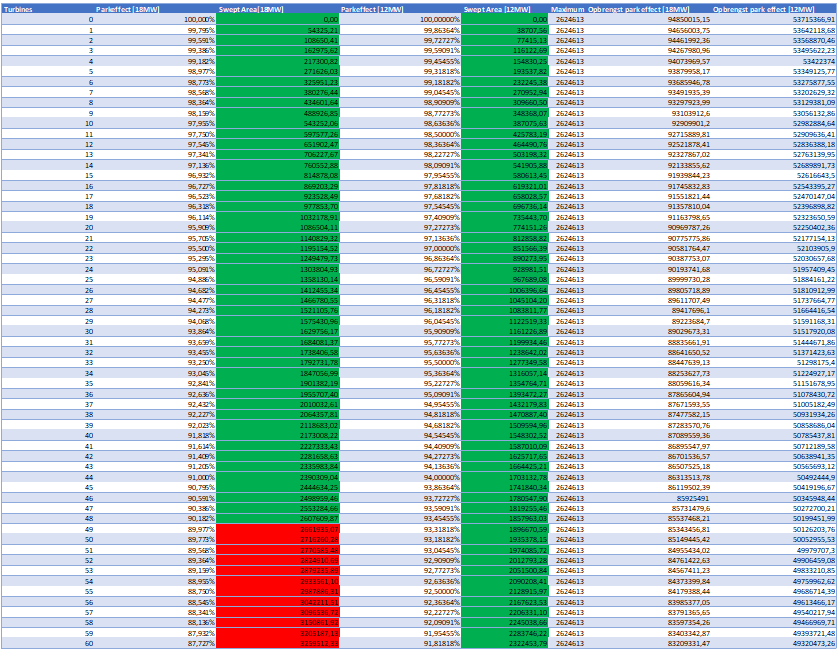
\includegraphics[width=1\textwidth]{IMG/data/overzicht/Parkeffect.PNG}
\caption{Gegevens: Aantal turbines, Parkeffect, Swept Area en Opbrengst park effect.}
\label{fig:Parkeffect_table}
\end{figure}

\begin{figure}[H]
\centering
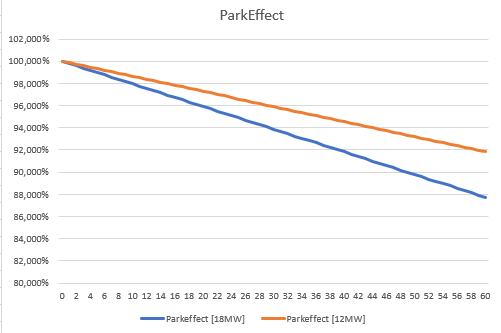
\includegraphics[width=0.7\textwidth]{IMG/data/overzicht/parkeffect_graph.PNG}
\caption{Plot: Parkeffect.}
\label{fig:ParkEffectGraph}
\end{figure}

Ten slotte kan met het parkeffect het daadwerklijke vermogen bepaald worden. Dit kan berekend worden door het parkeffect te berekenen voor het aantal turbines dat op de kavel komt. In dit geval gaat het om 48 turbines. Dus is het parkeffect: 

\begin{equation} \label{eq:12}
 Parkeffect_{18MW} = \frac{100-(P_{totaal}/A)}{100} = \frac{100-(864/88)}{100} = 0,902 = 90,2\%
\end{equation}
\myequations{Berekening: Parkeffect 18MW Turbine doorgerekend}

De jaarlijkse energieopbrengst inclusief het parkeffect is dan vrij simpel te berekenen met de formule: 
% \begin{equation} \label{eq:6}
% \text{Opbrengst 12MW kWh } t_{uren per jaar}\times VermogenPerWindsnelheid_{12MW}
% \end{equation}
% \begin{equation} \label{eq:7}
% \text{Opbrengst 18MW kWh } t_{uren per jaar}\times VermogenPerWindsnelheid_{18MW}
% \end{equation}


\begin{equation} \label{13}
\text{18MW Turbine: } OpbrengstParkeffect_{18MW}=Parkeffect_{18MW}\times E_{opbrengst,18MW} 
\end{equation}
\myequations{Berekening: Opbrengst Parkeffect 18MW Turbine}

\begin{equation} \label{14}
OpbrengstParkeffect_{18MW}=0,902\times 94850015 = 85.554.713kWh 
\end{equation}
\myequations{Berekening: Opbrengst Parkeffect 18MW Turbine}

\subsection{Configuratie 2 (12MW)}
Voor configuratie 2 zijn de meeste berekeningen al uitgevoerd bij configuratie 1. Ook is het verschil duidelijk te zien in de figuren en is voor elke formule het alternatief gegeven voor de turbine van configuratie 2. 

De energieopbrengst inclusief parkeffect zal hieronder worden berekend voor de windturbine van 12MW. 

\begin{equation} \label{eq:15}
 Parkeffect_{12MW} = \frac{100-(P_{totaal}/A)}{100} = \frac{100-((60\times 12)/88)}{100} = 0,918 = 91,8\%
\end{equation}
\myequations{Berekening: Parkeffect 12MW Turbine doorgerekend}

\begin{equation} \label{eq:16}
OpbrengstParkeffect_{12MW}=Parkeffect_{12MW}\times E_{opbrengst,12MW}
\end{equation}
\myequations{Berekening: Opbrengst Parkeffect 12MW Turbine}

\begin{equation} \label{eq:17}
OpbrengstParkeffect_{12MW}= 0,918\times 53715367 = 49.320.473 kWh
\end{equation}
\myequations{Berekening: Opbrengst Parkeffect 12MW Turbine}

Het verschil in jaarlijkse energieopbrengst, inclusief parkeffect, tussen de twee configuraties is dus \(85.554.713 - 49.320.473 = 36.234.240\) kWh aan energie per jaar. Dat is een zeer aanzienlijk getal. Dit is ook terug te zien in figuur \ref{fig:OpbrengstPark}

\begin{figure}[H]
\centering
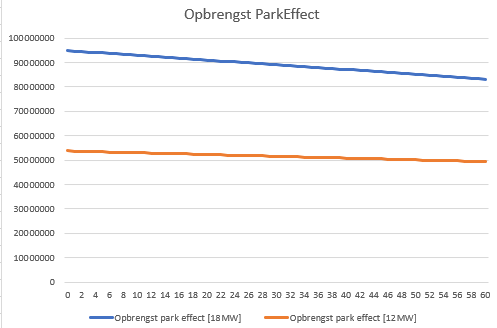
\includegraphics[width=0.7\textwidth]{IMG/data/overzicht/OpbrengstPark_graph.PNG}
\caption{Plot: OpbrengstPark.}
\label{fig:OpbrengstPark}
\end{figure}

\subsection{Vergelijking Configuratie 1 en Configuratie 2}

Bij het vergelijken van Configuratie 1 (18MW) met Configuratie 2 (12MW) zijn verschillende elektrotechnische aspecten van belang. 

\subsubsection{Vermogensdichtheid}

De vermogensdichtheid (\(P_{\text{dichtheid}}\)) van Configuratie 1 wordt berekend als:

\begin{equation} \label{eq:18}
P_{\text{dichtheid18MW}} = \frac{{n_{\text{turbines}} \times P_{\text{turbine}}}}{{A_{\text{oppervlak}}}} = \frac{{48 \times 18}}{{88}} = 9,818 \, \text{MW/km}^2
\end{equation}
\myequations{Berekening: Opbrengst Parkeffect 12MW Turbine}

Voor Configuratie 2 is de vermogensdichtheid (\(P_{\text{dichtheid12MW}}\)):

\begin{equation} \label{eq:19}
P_{\text{dichtheid12MW}} = \frac{{n_{\text{turbines}} \times P_{\text{turbine}}}}{{A_{\text{oppervlak}}}} = \frac{{60 \times 12}}{{88}} = 8,182 \, \text{MW/km}^2
\end{equation}
\myequations{Berekening: Opbrengst Parkeffect 12MW Turbine}

Hieruit blijkt dat Configuratie 1 een hogere vermogensdichtheid heeft, wat kan bijdragen aan een efficiëntere energieopwekking.

\subsubsection{Parkeffect}

Het parkeffect (\(P_{\text{effect}}\)) wordt berekend volgens Formule (11). Voor Configuratie 1:

\begin{equation} \label{eq:20}
P_{\text{effect18MW}} = 100 - \left(\frac{{n_{\text{turbines} \times P_{\text{turbine}}}}}{{A}} \right) = 100 - \frac{{864}}{{88}} = 90,2\%
\end{equation}
\myequations{Berekening: Opbrengst Parkeffect 12MW Turbine}

Voor Configuratie 2:

\begin{equation} \label{eq:21}
P_{\text{effect12MW}} = 100 - \left(\frac{{n_{\text{turbines}} \times P_{\text{turbine}}}}{{A}} \right) = 100 - \frac{{720}}{{88}} = 91,8\%
\end{equation}
\myequations{Berekening: Opbrengst Parkeffect 12MW Turbine}

Opmerkelijk is dat Configuratie 2 een hoger parkeffect heeft, wat kan wijzen op een efficiënter gebruik van de beschikbare ruimte.

\subsubsection{Jaarlijkse Energieopbrengst}

De jaarlijkse energieopbrengst wordt beïnvloed door zowel de vermogensdichtheid als het parkeffect. Voor Configuratie 1:

\begin{equation} \label{eq:22}
\text{Opbrengst}_{\text{effect18MW}} = P_{\text{effect18MW}} \times \text{E}_{\text{opbrengst,18MW}} = 0,902 \times 85.554.713 \, \text{kWh} = 77.151.870 \, \text{kWh}
\end{equation}
\myequations{Berekening: Opbrengst Parkeffect 12MW Turbine}

Voor Configuratie 2:

\begin{equation} \label{eq:23}
\text{Opbrengst}_{\text{effect12MW}} = P_{\text{effect12MW}} \times \text{E}_{\text{opbrengst,12MW}} = 0,918 \times 49.320.473 \, \text{kWh} = 45.255.460 \, \text{kWh}
\end{equation}
\myequations{Berekening: Opbrengst Parkeffect 12MW Turbine}

Hieruit blijkt dat Configuratie 1 een hogere jaarlijkse energieopbrengst heeft, wat suggereert dat het, ondanks een lager parkeffect, een efficiënter gebruik maakt van de beschikbare energiebron.

\section{Indeling van Windturbines en Bekabeling}
\subsection{Kavelindeling}
Voor de kavelindeling is er gekozen voor 48 turbines per kavel, omdat dit het maximale bereik van onze swept area is. Het maximale oppervlak volgens het kavelbesluit is vastgesteld op 2624613 m\textsuperscript{2}, en met 48 turbines wordt 2607609,87 m\textsuperscript{2} beslagen. Elke turbine heeft een oppervlakte van 54325,21 m\textsuperscript{2}, berekend met de formule:

\begin{equation} \label{eq:25}
\text{{Swept area per turbine}} = \pi \left(\frac{{\text{{Rotor diameter (m)}}}}{2}\right)^2
\end{equation}
\myequations{Berekening: Swept area per turbine}

Waarbij de rotor diameter gelijk is aan 263 m volgens de datasheet van NREL 18MW.\cite{NREL_turbine_documentatie}

De plaatsing van turbines is zo gedaan dat alle obstakels in figuur \ref{fig:windparkitems} worden vermeden. Ook zijn er een aantal objecten verwijderd (zie figuur \ref{fig:windparkturbines} om ruimte te maken voor de turbines met bekabeling.
\begin{table}[h]
    \centering
    \begin{tabular}{|c|c|}
        \hline
        \textbf{Point} & \textbf{Function} \\
        \hline
        Q3 P6C & Removed \\
        \hline
        BH01 & Removed \\
        \hline
        BH06 & Removed \\
        \hline
        BH08 & Removed \\
        \hline
        BH09 & Removed \\
        \hline
        BH11 & Removed \\
        \hline
        Q4 & Removed \\
        \hline
        BH12 & Removed \\
        \hline
    \end{tabular}
    \caption{Example of Removed Items}
    \label{tab:removed-items}
\end{table}

De turbine-plaatsing is ontworpen met voldoende ruimte tussen de turbines om het parkeffect te minimaliseren. De configuratie van de 48 turbines per kavel is te zien in figuur \ref{fig:windparkturbines}.
\begin{figure}[h]
    \centering
    \begin{subfigure}{0.5\textwidth}
        \centering
        \setlength{\fboxsep}{0pt}  % Set the padding of the \fbox to zero
    \colorbox{darkgray}{\fbox{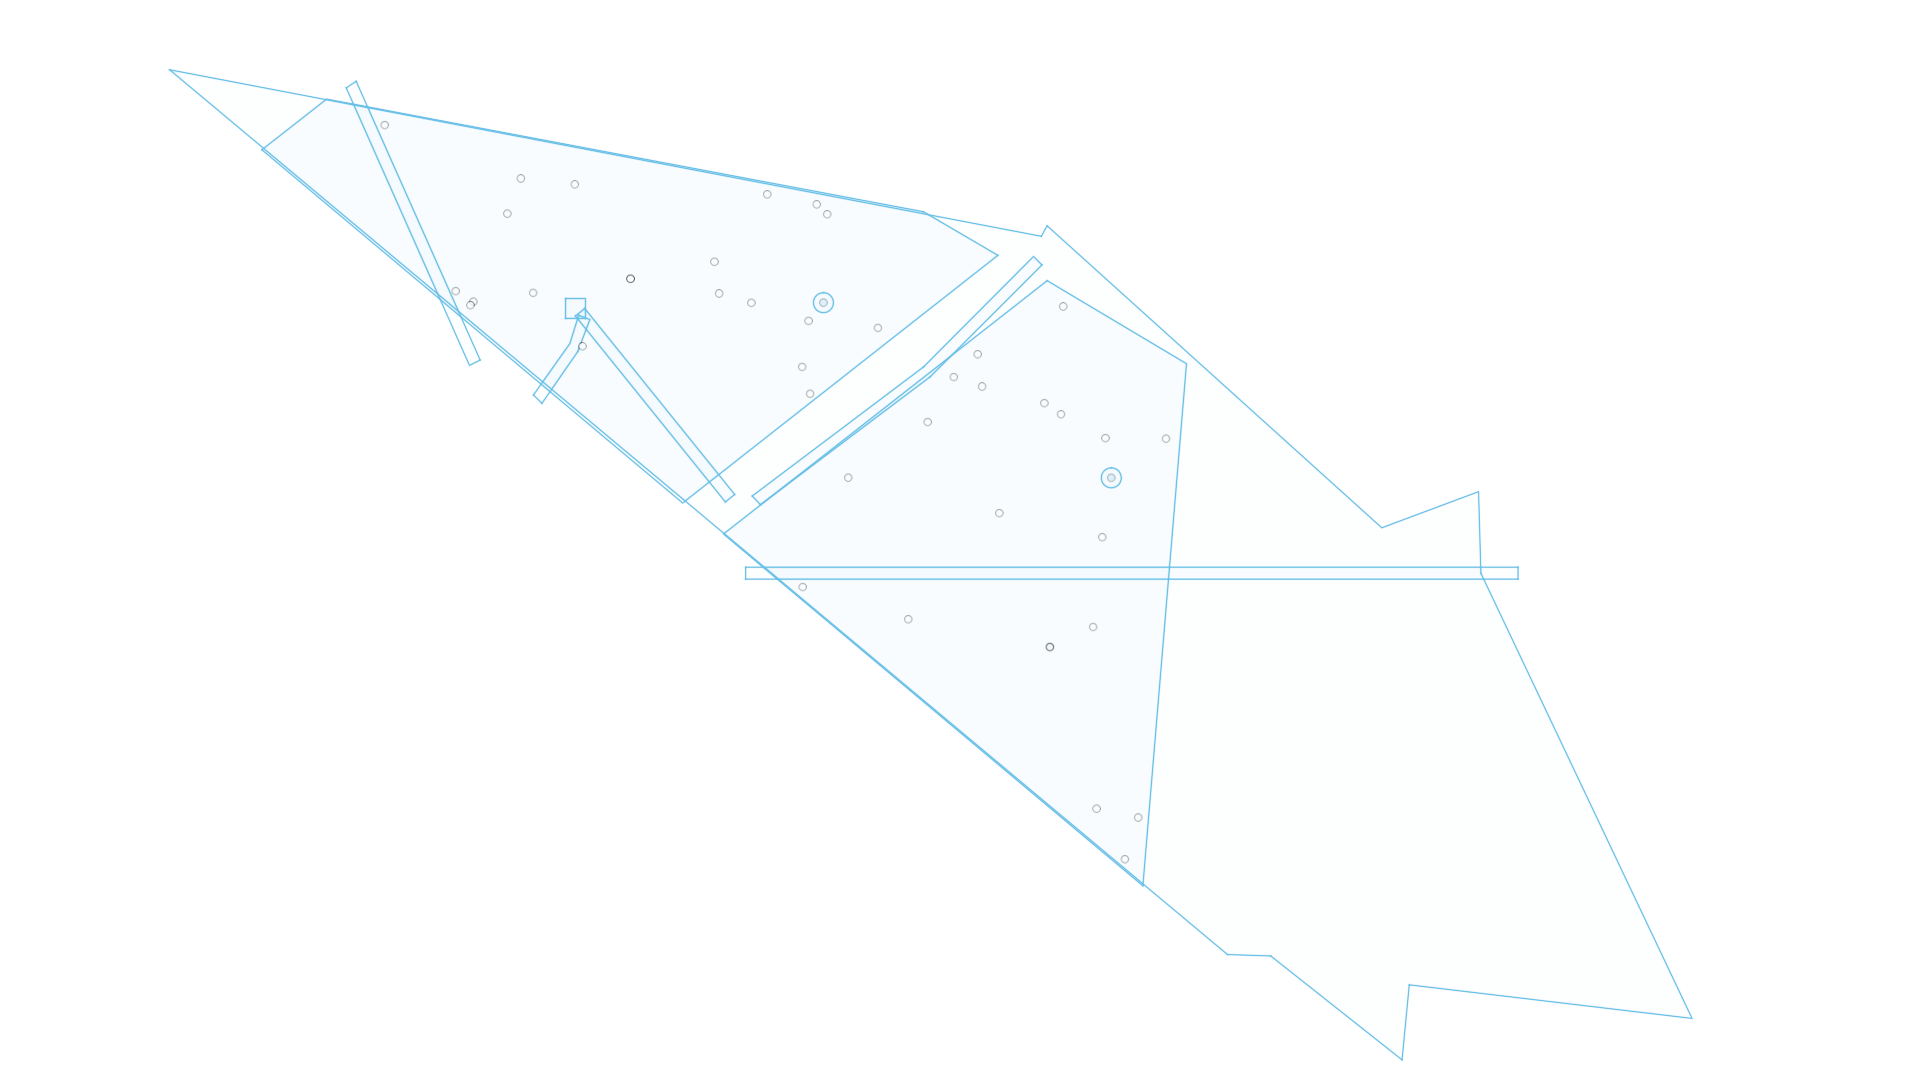
\includegraphics[width=0.5\textwidth, angle=270]{IMG/Kavelindeling/Windpark v30_BG.png}}}
        \caption{Alle obstakels aanwezig in kavels.}
        \label{fig:windparkitems}
    \end{subfigure}%
    \begin{subfigure}{0.5\textwidth}
        \centering
        \setlength{\fboxsep}{0pt}  % Set the padding of the \fbox to zero
    \colorbox{darkgray}{\fbox{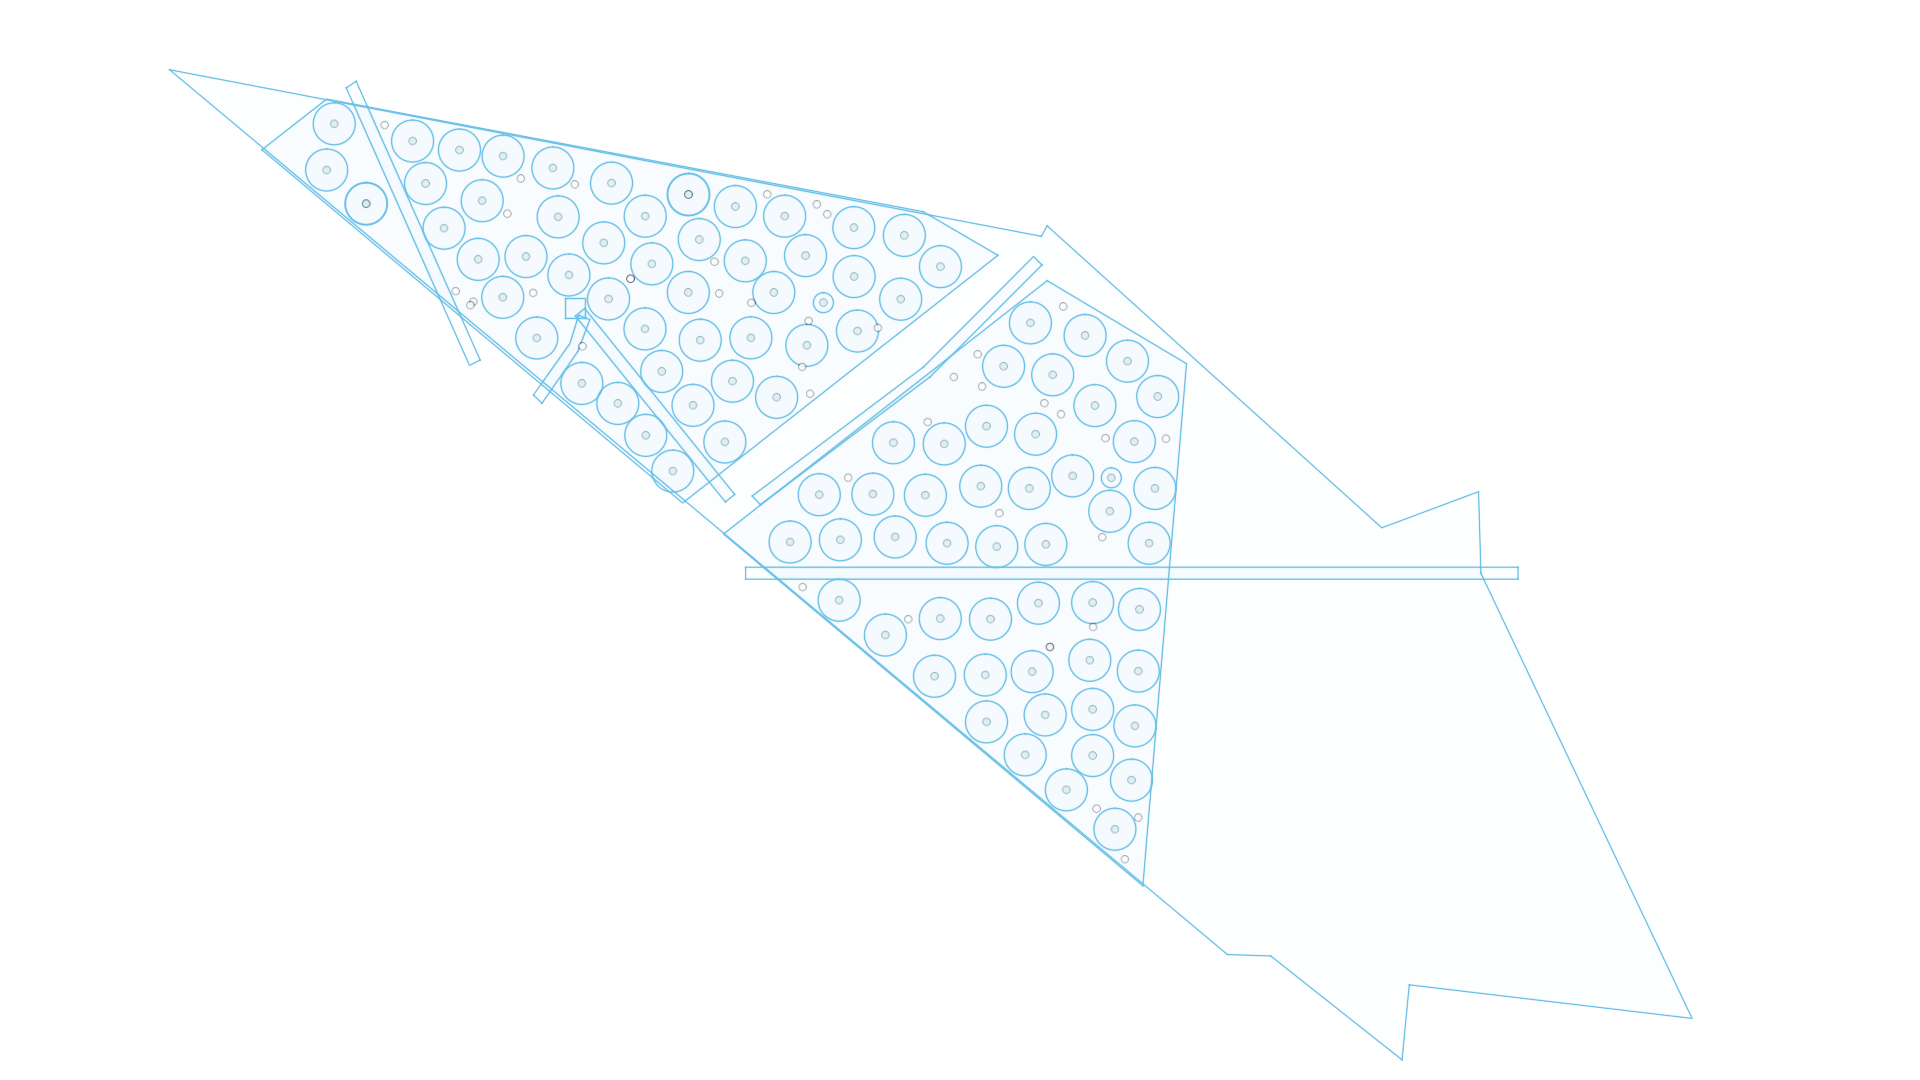
\includegraphics[width=0.5\textwidth, angle=270]{IMG/Kavelindeling/Windpark v30turbines.png}}}
        \caption{Alle obstakels en geplaatste turbines.}
        \label{fig:windparkturbines}
    \end{subfigure}
    \caption{Gegevens van het windpark.}
    \label{fig:windpark}
\end{figure}


\subsection{Bekabeling en Vermogen}
De tijdelijk gekozen ABB-kabel is ontworpen voor 66 kV (66000 V). Volgens de datasheet van ABB kan deze kabel maximaal 825 ampère overbrengen.\cite{Kabel_ABB} Elke turbine levert een vermogen van 18 MW. De formule voor het berekenen van het maximale vermogen per kabel is:

\begin{equation} \label{eq:26}
\text{{Maximaal vermogen per kabel}} = \left(\frac{{\text{{Spanning}}}}{{\sqrt{3}}}\right) \times 3 \times \text{{Stroom}} \times \text{{Formfactor}}
\end{equation} \myequations{Berekening: Maximaal vermogen per kabel}

Met een formfactor van 0,85 wordt dit:

\begin{equation} \label{eq:27}
\left(\frac{{66000}}{{\sqrt{3}}}\right) \times 3 \times 825 \times 0,85 = 80.163.641,50 Watt
\end{equation} \myequations{Berekening: Veiligheidsfactor}

Dit is het maximale vermogen dat er per kabel/tak kan worden getransporteerd. Door de formule \(\frac{{\text{{Turbine MW}}}}{{\text{{Tak MW}}}}\) toe te passen, word verkregen dat veilig 4 turbines per kabel naar het TenneT-station kunnen worden verbonden.

De bekabeling is weergegeven in figuur \ref{fig:windparktotaal}.

\begin{figure}[H]
    \centering
    \setlength{\fboxsep}{0pt}  % Set the padding of the \fbox to zero
    \colorbox{darkgray}{\fbox{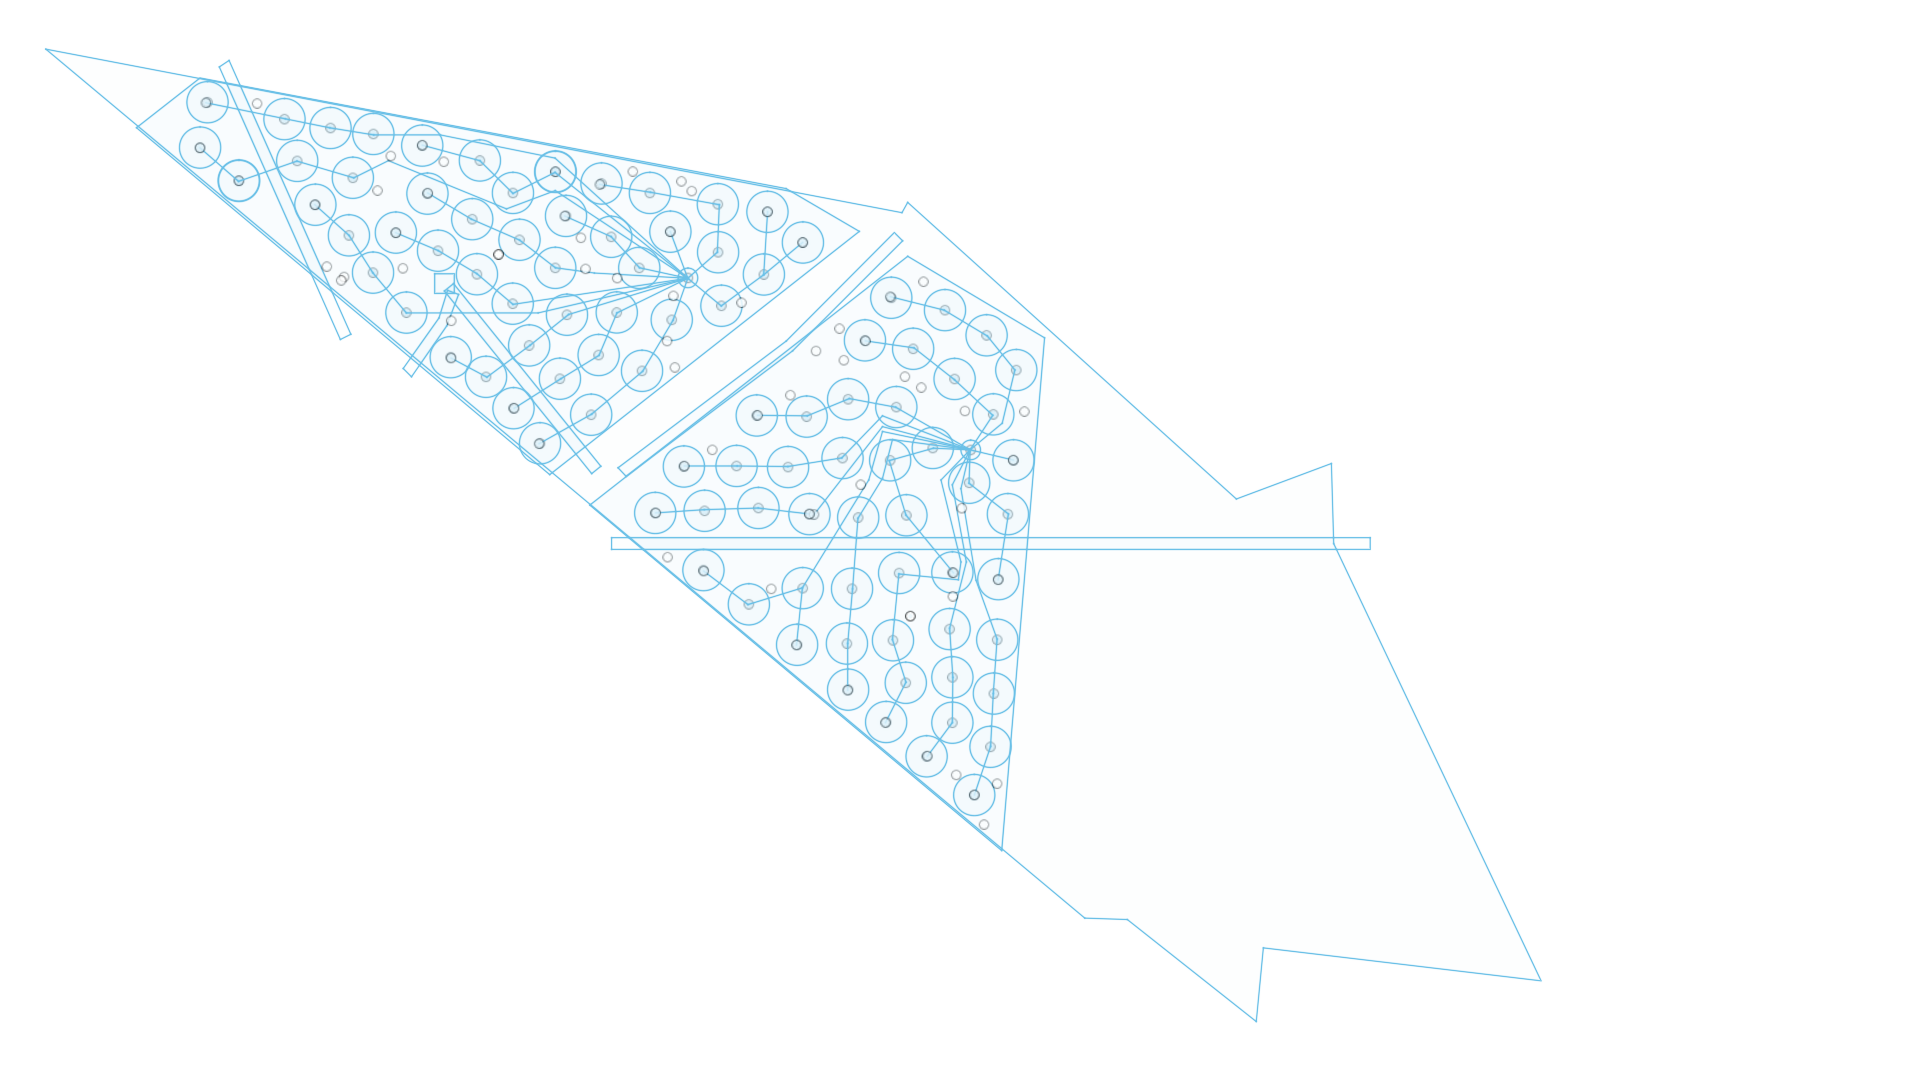
\includegraphics[width=0.5\textwidth, angle=270]{IMG/Kavelindeling/Windpark v30.png}}}
    \caption{Alle obstakels, geplaatste turbines en kabels.}
    \label{fig:windparktotaal}
\end{figure}

\subsection{Lengte en Kenmerken van Kabels}
Volgens de heer Dhirhadj Djairam kan elke tak beschouwd worden als één kabel. Door alle lengtes op te tellen, is het mogelijk om de weerstanden, capaciteiten en inducties van de kabels van kavel VI en VII berekenen. De specifieke weerstand van de kabel wordt bepaald door de formule:

\begin{equation} \label{eq:28}
\text{{Weerstand kabel}} = \frac{{\text{{Lengte kabel}} \times \text{{Soortelijke weerstand}}}}{{\text{{Doorsnede kabel}}}}
\end{equation} \myequations{Berekening: Specifieke weerstand kabel}

De capaciteit van de kabel wordt gegeven door\cite{Kabel_ABB}:

\begin{equation} \label{eq:29}
\text{{Capaciteit kabel}} = \text{{Lengte kabel}} \times \text{{Capaciteit per km}}
\end{equation} \myequations{Berekening: Capaciteit kabel}

En de inductie van de kabel is\cite{Kabel_ABB}:

\begin{equation} \label{eq:30}
\text{{Inductie kabel}} = \text{{Lengte kabel}} \times \text{{Inductie per km}}
\end{equation} \myequations{Berekening: Inductie kabel}

Door deze formules toe te passen, kunnen de gegevens voor kabel VI en VII worden ingevuld, weergegeven in tabel \ref{tab:Kavel VI - Kabel data} en tabel \ref{tab:Kavel VII - Kabel data}.

\begin{table}[h]
\resizebox{\textwidth}{!}{
\begin{tabular}{|llllllllllllll|}
\hline
\rowcolor[HTML]{9B9B9B} 
\multicolumn{14}{|c|}{\cellcolor[HTML]{9B9B9B}\textbf{Kavel VI}} \\ \hline
\rowcolor[HTML]{C0C0C0} 
\multicolumn{1}{|l|}{\cellcolor[HTML]{C0C0C0}\textit{\textbf{Kabel}}} &
  \multicolumn{1}{l|}{\cellcolor[HTML]{C0C0C0}\textit{\textbf{1}}} &
  \multicolumn{1}{l|}{\cellcolor[HTML]{C0C0C0}\textit{\textbf{2}}} &
  \multicolumn{1}{l|}{\cellcolor[HTML]{C0C0C0}\textit{\textbf{3}}} &
  \multicolumn{1}{l|}{\cellcolor[HTML]{C0C0C0}\textit{\textbf{4}}} &
  \multicolumn{1}{l|}{\cellcolor[HTML]{C0C0C0}\textit{\textbf{5}}} &
  \multicolumn{1}{l|}{\cellcolor[HTML]{C0C0C0}\textit{\textbf{6}}} &
  \multicolumn{1}{l|}{\cellcolor[HTML]{C0C0C0}\textit{\textbf{7}}} &
  \multicolumn{1}{l|}{\cellcolor[HTML]{C0C0C0}\textit{\textbf{8}}} &
  \multicolumn{1}{l|}{\cellcolor[HTML]{C0C0C0}\textit{\textbf{9}}} &
  \multicolumn{1}{l|}{\cellcolor[HTML]{C0C0C0}\textit{\textbf{10}}} &
  \multicolumn{1}{l|}{\cellcolor[HTML]{C0C0C0}\textit{\textbf{11}}} &
  \multicolumn{1}{l|}{\cellcolor[HTML]{C0C0C0}\textit{\textbf{12}}} &
  \textit{\textbf{13}} \\ \hline
\rowcolor[HTML]{FFFFFF} 
\multicolumn{1}{|l|}{\cellcolor[HTML]{EFEFEF}\textbf{Afstand} {[}\textit{KM}{]}} &
  \multicolumn{1}{l|}{\cellcolor[HTML]{FFFFFF}5,35} &
  \multicolumn{1}{l|}{\cellcolor[HTML]{FFFFFF}5,30} &
  \multicolumn{1}{l|}{\cellcolor[HTML]{FFFFFF}1,27} &
  \multicolumn{1}{l|}{\cellcolor[HTML]{FFFFFF}13,60} &
  \multicolumn{1}{l|}{\cellcolor[HTML]{FFFFFF}8,23} &
  \multicolumn{1}{l|}{\cellcolor[HTML]{FFFFFF}14,00} &
  \multicolumn{1}{l|}{\cellcolor[HTML]{FFFFFF}3,63} &
  \multicolumn{1}{l|}{\cellcolor[HTML]{FFFFFF}7,18} &
  \multicolumn{1}{l|}{\cellcolor[HTML]{FFFFFF}8,03} &
  \multicolumn{1}{l|}{\cellcolor[HTML]{FFFFFF}10,91} &
  \multicolumn{1}{l|}{\cellcolor[HTML]{FFFFFF}6,84} &
  \multicolumn{1}{l|}{\cellcolor[HTML]{FFFFFF}3,72} &
  5,88 \\ \hline
\rowcolor[HTML]{EFEFEF} 
\multicolumn{1}{|l|}{\cellcolor[HTML]{EFEFEF}\textbf{Weerstand} {[}\textit{\(\Omega\)}{]}} &
  \multicolumn{1}{l|}{\cellcolor[HTML]{EDEDED}0,09} &
  \multicolumn{1}{l|}{\cellcolor[HTML]{EDEDED}0,09} &
  \multicolumn{1}{l|}{\cellcolor[HTML]{EDEDED}0,02} &
  \multicolumn{1}{l|}{\cellcolor[HTML]{EDEDED}0,24} &
  \multicolumn{1}{l|}{\cellcolor[HTML]{EDEDED}0,14} &
  \multicolumn{1}{l|}{\cellcolor[HTML]{EDEDED}0,25} &
  \multicolumn{1}{l|}{\cellcolor[HTML]{EDEDED}0,06} &
  \multicolumn{1}{l|}{\cellcolor[HTML]{EDEDED}0,13} &
  \multicolumn{1}{l|}{\cellcolor[HTML]{EDEDED}0,14} &
  \multicolumn{1}{l|}{\cellcolor[HTML]{EDEDED}0,19} &
  \multicolumn{1}{l|}{\cellcolor[HTML]{EDEDED}0,12} &
  \multicolumn{1}{l|}{\cellcolor[HTML]{EDEDED}0,07} &
  0,10 \\ \hline
\rowcolor[HTML]{FFFFFF} 
\multicolumn{1}{|l|}{\cellcolor[HTML]{FFFFFF}\textbf{Capaciteit} {[}\textit{uF}{]}} &
  \multicolumn{1}{l|}{\cellcolor[HTML]{FFFFFF}2,03} &
  \multicolumn{1}{l|}{\cellcolor[HTML]{FFFFFF}2,01} &
  \multicolumn{1}{l|}{\cellcolor[HTML]{FFFFFF}0,48} &
  \multicolumn{1}{l|}{\cellcolor[HTML]{FFFFFF}5,17} &
  \multicolumn{1}{l|}{\cellcolor[HTML]{FFFFFF}3,13} &
  \multicolumn{1}{l|}{\cellcolor[HTML]{FFFFFF}5,32} &
  \multicolumn{1}{l|}{\cellcolor[HTML]{FFFFFF}1,38} &
  \multicolumn{1}{l|}{\cellcolor[HTML]{FFFFFF}2,73} &
  \multicolumn{1}{l|}{\cellcolor[HTML]{FFFFFF}3,05} &
  \multicolumn{1}{l|}{\cellcolor[HTML]{FFFFFF}4,15} &
  \multicolumn{1}{l|}{\cellcolor[HTML]{FFFFFF}2,60} &
  \multicolumn{1}{l|}{\cellcolor[HTML]{FFFFFF}1,42} &
  2,24 \\ \hline
\rowcolor[HTML]{EDEDED} 
\multicolumn{1}{|l|}{\cellcolor[HTML]{EFEFEF}\textbf{Inductie} {[}\textit{mH}{]}} &
  \multicolumn{1}{l|}{\cellcolor[HTML]{EDEDED}1,66} &
  \multicolumn{1}{l|}{\cellcolor[HTML]{EDEDED}1,64} &
  \multicolumn{1}{l|}{\cellcolor[HTML]{EDEDED}0,39} &
  \multicolumn{1}{l|}{\cellcolor[HTML]{EDEDED}4,22} &
  \multicolumn{1}{l|}{\cellcolor[HTML]{EDEDED}2,55} &
  \multicolumn{1}{l|}{\cellcolor[HTML]{EDEDED}4,34} &
  \multicolumn{1}{l|}{\cellcolor[HTML]{EDEDED}1,12} &
  \multicolumn{1}{l|}{\cellcolor[HTML]{EDEDED}2,22} &
  \multicolumn{1}{l|}{\cellcolor[HTML]{EDEDED}2,49} &
  \multicolumn{1}{l|}{\cellcolor[HTML]{EDEDED}3,38} &
  \multicolumn{1}{l|}{\cellcolor[HTML]{EDEDED}2,12} &
  \multicolumn{1}{l|}{\cellcolor[HTML]{EDEDED}1,15} &
  1,82 \\ \hline
\end{tabular}
}
\caption{Kabeldata van kavel VI}
\label{tab:Kavel VI - Kabel data}
\end{table}


\begin{table}[h]
\resizebox{\textwidth}{!}{
\begin{tabular}{|lllllllllllllll|}
\hline
\rowcolor[HTML]{9B9B9B} 
\multicolumn{15}{|c|}{\cellcolor[HTML]{9B9B9B}\textbf{Kavel VII}} \\ \hline
\rowcolor[HTML]{C0C0C0} 
\multicolumn{1}{|l|}{\cellcolor[HTML]{C0C0C0}\textit{\textbf{Kabel}}} &
  \multicolumn{1}{l|}{\cellcolor[HTML]{C0C0C0}\textit{\textbf{1}}} &
  \multicolumn{1}{l|}{\cellcolor[HTML]{C0C0C0}\textit{\textbf{2}}} &
  \multicolumn{1}{l|}{\cellcolor[HTML]{C0C0C0}\textit{\textbf{3}}} &
  \multicolumn{1}{l|}{\cellcolor[HTML]{C0C0C0}\textit{\textbf{4}}} &
  \multicolumn{1}{l|}{\cellcolor[HTML]{C0C0C0}\textit{\textbf{5}}} &
  \multicolumn{1}{l|}{\cellcolor[HTML]{C0C0C0}\textit{\textbf{6}}} &
  \multicolumn{1}{l|}{\cellcolor[HTML]{C0C0C0}\textit{\textbf{7}}} &
  \multicolumn{1}{l|}{\cellcolor[HTML]{C0C0C0}\textit{\textbf{8}}} &
  \multicolumn{1}{l|}{\cellcolor[HTML]{C0C0C0}\textit{\textbf{9}}} &
  \multicolumn{1}{l|}{\cellcolor[HTML]{C0C0C0}\textit{\textbf{10}}} &
  \multicolumn{1}{l|}{\cellcolor[HTML]{C0C0C0}\textit{\textbf{11}}} &
  \multicolumn{1}{l|}{\cellcolor[HTML]{C0C0C0}\textit{\textbf{12}}} &
  \multicolumn{1}{l|}{\cellcolor[HTML]{C0C0C0}\textit{\textbf{13}}} &
  \cellcolor[HTML]{C0C0C0}\textit{\textbf{14}} \\ \hline
\rowcolor[HTML]{FFFFFF} 
\multicolumn{1}{|l|}{\cellcolor[HTML]{FFFFFF}\textbf{Afstand} {[}\textit{KM}{]}} &
  \multicolumn{1}{l|}{\cellcolor[HTML]{FFFFFF}6,27} &
  \multicolumn{1}{l|}{\cellcolor[HTML]{FFFFFF}4,95} &
  \multicolumn{1}{l|}{\cellcolor[HTML]{FFFFFF}5,81} &
  \multicolumn{1}{l|}{\cellcolor[HTML]{FFFFFF}7,92} &
  \multicolumn{1}{l|}{\cellcolor[HTML]{FFFFFF}9,08} &
  \multicolumn{1}{l|}{\cellcolor[HTML]{FFFFFF}14,13} &
  \multicolumn{1}{l|}{\cellcolor[HTML]{FFFFFF}8,61} &
  \multicolumn{1}{l|}{\cellcolor[HTML]{FFFFFF}8,61} &
  \multicolumn{1}{l|}{\cellcolor[HTML]{FFFFFF}5,46} &
  \multicolumn{1}{l|}{\cellcolor[HTML]{FFFFFF}9,18} &
  \multicolumn{1}{l|}{\cellcolor[HTML]{FFFFFF}8,21} &
  \multicolumn{1}{l|}{\cellcolor[HTML]{FFFFFF}9,02} &
  \multicolumn{1}{l|}{\cellcolor[HTML]{FFFFFF}3,82} &
  1,13 \\ \hline
\rowcolor[HTML]{EFEFEF} 
\multicolumn{1}{|l|}{\cellcolor[HTML]{EFEFEF}\textbf{Weerstand} {[}\textit{\(\Omega\)}{]}} &
  \multicolumn{1}{l|}{\cellcolor[HTML]{EFEFEF}0,11} &
  \multicolumn{1}{l|}{\cellcolor[HTML]{EFEFEF}0,09} &
  \multicolumn{1}{l|}{\cellcolor[HTML]{EFEFEF}0,10} &
  \multicolumn{1}{l|}{\cellcolor[HTML]{EFEFEF}0,14} &
  \multicolumn{1}{l|}{\cellcolor[HTML]{EFEFEF}0,16} &
  \multicolumn{1}{l|}{\cellcolor[HTML]{EFEFEF}0,25} &
  \multicolumn{1}{l|}{\cellcolor[HTML]{EFEFEF}0,15} &
  \multicolumn{1}{l|}{\cellcolor[HTML]{EFEFEF}0,15} &
  \multicolumn{1}{l|}{\cellcolor[HTML]{EFEFEF}0,10} &
  \multicolumn{1}{l|}{\cellcolor[HTML]{EFEFEF}0,16} &
  \multicolumn{1}{l|}{\cellcolor[HTML]{EFEFEF}0,14} &
  \multicolumn{1}{l|}{\cellcolor[HTML]{EFEFEF}0,16} &
  \multicolumn{1}{l|}{\cellcolor[HTML]{EFEFEF}0,07} &
  0,02 \\ \hline
\rowcolor[HTML]{FFFFFF} 
\multicolumn{1}{|l|}{\cellcolor[HTML]{FFFFFF}\textbf{Capaciteit} {[}\textit{uF}{]}} &
  \multicolumn{1}{l|}{\cellcolor[HTML]{FFFFFF}2,38} &
  \multicolumn{1}{l|}{\cellcolor[HTML]{FFFFFF}1,88} &
  \multicolumn{1}{l|}{\cellcolor[HTML]{FFFFFF}2,21} &
  \multicolumn{1}{l|}{\cellcolor[HTML]{FFFFFF}3,01} &
  \multicolumn{1}{l|}{\cellcolor[HTML]{FFFFFF}3,45} &
  \multicolumn{1}{l|}{\cellcolor[HTML]{FFFFFF}5,37} &
  \multicolumn{1}{l|}{\cellcolor[HTML]{FFFFFF}3,27} &
  \multicolumn{1}{l|}{\cellcolor[HTML]{FFFFFF}3,27} &
  \multicolumn{1}{l|}{\cellcolor[HTML]{FFFFFF}2,08} &
  \multicolumn{1}{l|}{\cellcolor[HTML]{FFFFFF}3,49} &
  \multicolumn{1}{l|}{\cellcolor[HTML]{FFFFFF}3,12} &
  \multicolumn{1}{l|}{\cellcolor[HTML]{FFFFFF}3,43} &
  \multicolumn{1}{l|}{\cellcolor[HTML]{FFFFFF}1,45} &
  0,43 \\ \hline
\rowcolor[HTML]{EFEFEF} 
\multicolumn{1}{|l|}{\cellcolor[HTML]{EFEFEF}\textbf{Inductie} {[}\textit{mH}{]}} &
  \multicolumn{1}{l|}{\cellcolor[HTML]{EFEFEF}1,94} &
  \multicolumn{1}{l|}{\cellcolor[HTML]{EFEFEF}1,53} &
  \multicolumn{1}{l|}{\cellcolor[HTML]{EFEFEF}1,80} &
  \multicolumn{1}{l|}{\cellcolor[HTML]{EFEFEF}2,45} &
  \multicolumn{1}{l|}{\cellcolor[HTML]{EFEFEF}2,81} &
  \multicolumn{1}{l|}{\cellcolor[HTML]{EFEFEF}4,38} &
  \multicolumn{1}{l|}{\cellcolor[HTML]{EFEFEF}2,67} &
  \multicolumn{1}{l|}{\cellcolor[HTML]{EFEFEF}2,67} &
  \multicolumn{1}{l|}{\cellcolor[HTML]{EFEFEF}1,69} &
  \multicolumn{1}{l|}{\cellcolor[HTML]{EFEFEF}2,85} &
  \multicolumn{1}{l|}{\cellcolor[HTML]{EFEFEF}2,55} &
  \multicolumn{1}{l|}{\cellcolor[HTML]{EFEFEF}2,80} &
  \multicolumn{1}{l|}{\cellcolor[HTML]{EFEFEF}1,19} &
  0,35 \\ \hline
\end{tabular}
}
\caption{Kabeldata van kavel VII}
\label{tab:Kavel VII - Kabel data}
\end{table}

\section{Wat zijn de te verwachte stromen door de kabels en de bijbehorende belangrijke gegevens?}

De stromen die door de kabels zullen stromen hangt af van meerdere factoren. Ten eerste is het aantal turbines van belang. In het windpark zijn, zoals in het vorige hoofdstuk aangegeven, de turbines met groepen van vier, drie of één via een inter array kabel verbonden met het TenneT-station. Het totale werkelijk vermogen P wat dan door de kabel zal moeten verschilt dus van 72MW tot 18MW. Om de stromen te kunnen berekenen zal voor de volgende berekening worden aangenomen dat het totale werkelijk vermogen P overeen komt met het totale schijnbaar vermogen S. S zal voor de verschillende aantallen turbines dus drie waardes hebben. 
De verwachte stromen per fase kabel zijn te berekenen door middel van formule \ref{eq:312}. 

\begin{equation} \label{eq:312}
I\textsubscript{fase} = \frac{S/3}{U/ \sqrt{3}} = \frac{72.000.000/3}{66.000/ \sqrt{3}} = 629,84 A
\end{equation}
\myequations{Berekening: Ifase}

In formule \ref{eq:30} wordt de capacitieve reactantie (\(X_c\)) berekend met behulp van de opgegeven formule, waarbij de capaciteit terug te vinden is in tabel \ref{tab:Kavel VI - Kabel data} en tabel \ref{tab:Kavel VII - Kabel data}.

% Vergelijking 30: Berekening van Xc
\begin{equation} \label{eq:30}
X_c = \frac{1}{{100 \times \pi \times \text{{Capaciteit}}}}
\end{equation}
\myequations{Berekening: Xc}

In formule \ref{eq:31} wordt de capacitieve reactantie (\(X_c\)) berekend met behulp van de opgegeven formule, waarbij de inductantie terug te vinden is in tabel \ref{tab:Kavel VI - Kabel data} en tabel \ref{tab:Kavel VII - Kabel data}.
% Vergelijking 31: Berekening van Xl
\begin{equation} \label{eq:31}
X_l = 100 \times \pi \times \text{{Inductie}}
\end{equation}
\myequations{Berekening: Xl}

In formule \ref{eq:32} wordt de impedantie (\(Z\)) met behulp van de capacitieve reactantie (\(X_c\)), inductieve reactantie (\(X_l\)) en weerstand (\(R\)).
% Vergelijking 32: Berekening van Impedantie
\begin{equation} \label{eq:32}
Z = \sqrt{{(X_c - X_l)^2 + R^2}}
\end{equation}
\myequations{Berekening: Z}


In formule \ref{eq:33} worden de verliezen met behulp van de fase-spanning (\(\text{{Vfase}}\)) en impedantie (\(Z\)).
% Vergelijking 33: Berekening van Verliezen
\begin{equation} \label{eq:33}
\text{{Verliezen}} = \frac{{\text{{Vfase}}}}{{Z}}
\end{equation}
\myequations{Berekening: Verliezen}


In formule \ref{eq:34} wordt de fase-spanning (\(\text{{Vfase}}\)) met behulp van de opgegeven formule.
% Vergelijking 34: Berekening van Vfase
\begin{equation} \label{eq:34}
\text{{Vfase}} = \frac{{66000}}{{\sqrt{3}}}
\end{equation}
\myequations{Berekening: Vfase}


In formule \ref{eq:35} wordt de stroom per kabel met behulp van het vermogen per turbine, het aantal turbines en de fase-spanning.

% Vergelijking 35: Berekening van Stroom per kabel
\begin{equation} \label{eq:35}
\text{{Stroom per kabel}} = \frac{{\text{{Vermogen per turbine}} \times \text{{Aantal turbines}}}}{{\frac{{66000}}{{\sqrt{3}}}}} = \frac{{18000000 \times \text{{nTurbines}}}}{{\frac{{66000}}{{\sqrt{3}}}}}
\end{equation}
\myequations{Berekening: Stroom per kabel}

In formule \ref{eq:36} wordt de netto stroom door de verliezen af te trekken van de stroom per kabel.
% Vergelijking 36: Berekening van Netto stroom
\begin{equation} \label{eq:36}
\text{{Netto stroom}} = \text{{Stroom per kabel}} - \text{{Verliezen}}
\end{equation}
\myequations{Berekening: Netto stroom}


Met behulp van formule \ref{eq:30}, \ref{eq:31}, \ref{eq:32}, \ref{eq:33}, \ref{eq:34}, \ref{eq:35} en \ref{eq:36} kan tabel \ref{tab:Kavel VI - Kabel extra data} en tabel \ref{tab:Kavel VII - Kabel extra data} worden ingevuld.

\begin{table}[h]
\resizebox{\textwidth}{!}{
\begin{tabular}{|lrrrrrrrrrrrrrr|}
\hline
\rowcolor[HTML]{9B9B9B} 
\multicolumn{14}{|c|}{\cellcolor[HTML]{9B9B9B}\textbf{Kavel VI}} \\ \hline
\rowcolor[HTML]{C0C0C0} 
\multicolumn{1}{|l|}{\cellcolor[HTML]{C0C0C0}\textit{\textbf{Kabel nummer}}} &
  \multicolumn{1}{l|}{\cellcolor[HTML]{C0C0C0}\textit{\textbf{1}}} &
  \multicolumn{1}{l|}{\cellcolor[HTML]{C0C0C0}\textit{\textbf{2}}} &
  \multicolumn{1}{l|}{\cellcolor[HTML]{C0C0C0}\textit{\textbf{3}}} &
  \multicolumn{1}{l|}{\cellcolor[HTML]{C0C0C0}\textit{\textbf{4}}} &
  \multicolumn{1}{l|}{\cellcolor[HTML]{C0C0C0}\textit{\textbf{5}}} &
  \multicolumn{1}{l|}{\cellcolor[HTML]{C0C0C0}\textit{\textbf{6}}} &
  \multicolumn{1}{l|}{\cellcolor[HTML]{C0C0C0}\textit{\textbf{7}}} &
  \multicolumn{1}{l|}{\cellcolor[HTML]{C0C0C0}\textit{\textbf{8}}} &
  \multicolumn{1}{l|}{\cellcolor[HTML]{C0C0C0}\textit{\textbf{9}}} &
  \multicolumn{1}{l|}{\cellcolor[HTML]{C0C0C0}\textit{\textbf{10}}} &
  \multicolumn{1}{l|}{\cellcolor[HTML]{C0C0C0}\textit{\textbf{11}}} &
  \multicolumn{1}{l|}{\cellcolor[HTML]{C0C0C0}\textit{\textbf{12}}} &
  \textit{\textbf{13}} \\ \hline
\rowcolor[HTML]{FFFFFF} 
\multicolumn{1}{|l|}{\cellcolor[HTML]{A5A5A5}{\color[HTML]{FFFFFF} \textbf{Totaal (KM)}}} &
  \multicolumn{1}{l|}{\cellcolor[HTML]{FFFFFF}5,35} &
  \multicolumn{1}{l|}{\cellcolor[HTML]{FFFFFF}5,30} &
  \multicolumn{1}{l|}{\cellcolor[HTML]{FFFFFF}1,27} &
  \multicolumn{1}{l|}{\cellcolor[HTML]{FFFFFF}13,60} &
  \multicolumn{1}{l|}{\cellcolor[HTML]{FFFFFF}8,23} &
  \multicolumn{1}{l|}{\cellcolor[HTML]{FFFFFF}14,00} &
  \multicolumn{1}{l|}{\cellcolor[HTML]{FFFFFF}3,63} &
  \multicolumn{1}{l|}{\cellcolor[HTML]{FFFFFF}7,18} &
  \multicolumn{1}{l|}{\cellcolor[HTML]{FFFFFF}8,03} &
  \multicolumn{1}{l|}{\cellcolor[HTML]{FFFFFF}10,91} &
  \multicolumn{1}{l|}{\cellcolor[HTML]{FFFFFF}6,84} &
  \multicolumn{1}{l|}{\cellcolor[HTML]{FFFFFF}3,72} &
  5,88 \\ \hline
\rowcolor[HTML]{EFEFEF} 
\multicolumn{1}{|l|}{\cellcolor[HTML]{A5A5A5}{\color[HTML]{FFFFFF} \textbf{Weerstand (ohm)}}} &
  \multicolumn{1}{l|}{\cellcolor[HTML]{EFEFEF}0,09} &
  \multicolumn{1}{l|}{\cellcolor[HTML]{EFEFEF}0,09} &
  \multicolumn{1}{l|}{\cellcolor[HTML]{EFEFEF}0,02} &
  \multicolumn{1}{l|}{\cellcolor[HTML]{EFEFEF}0,24} &
  \multicolumn{1}{l|}{\cellcolor[HTML]{EFEFEF}0,14} &
  \multicolumn{1}{l|}{\cellcolor[HTML]{EFEFEF}0,25} &
  \multicolumn{1}{l|}{\cellcolor[HTML]{EFEFEF}0,06} &
  \multicolumn{1}{l|}{\cellcolor[HTML]{EFEFEF}0,13} &
  \multicolumn{1}{l|}{\cellcolor[HTML]{EFEFEF}0,14} &
  \multicolumn{1}{l|}{\cellcolor[HTML]{EFEFEF}0,19} &
  \multicolumn{1}{l|}{\cellcolor[HTML]{EFEFEF}0,12} &
  \multicolumn{1}{l|}{\cellcolor[HTML]{EFEFEF}0,07} &
  0,10 \\ \hline
\rowcolor[HTML]{FFFFFF} 
\multicolumn{1}{|l|}{\cellcolor[HTML]{A5A5A5}{\color[HTML]{FFFFFF} \textbf{Capaciteit (uF)}}} &
  \multicolumn{1}{l|}{\cellcolor[HTML]{FFFFFF}2,03} &
  \multicolumn{1}{l|}{\cellcolor[HTML]{FFFFFF}2,01} &
  \multicolumn{1}{l|}{\cellcolor[HTML]{FFFFFF}0,48} &
  \multicolumn{1}{l|}{\cellcolor[HTML]{FFFFFF}5,17} &
  \multicolumn{1}{l|}{\cellcolor[HTML]{FFFFFF}3,13} &
  \multicolumn{1}{l|}{\cellcolor[HTML]{FFFFFF}5,32} &
  \multicolumn{1}{l|}{\cellcolor[HTML]{FFFFFF}1,38} &
  \multicolumn{1}{l|}{\cellcolor[HTML]{FFFFFF}2,73} &
  \multicolumn{1}{l|}{\cellcolor[HTML]{FFFFFF}3,05} &
  \multicolumn{1}{l|}{\cellcolor[HTML]{FFFFFF}4,15} &
  \multicolumn{1}{l|}{\cellcolor[HTML]{FFFFFF}2,60} &
  \multicolumn{1}{l|}{\cellcolor[HTML]{FFFFFF}1,42} &
  2,24 \\ \hline
\rowcolor[HTML]{EFEFEF} 
\multicolumn{1}{|l|}{\cellcolor[HTML]{A5A5A5}{\color[HTML]{FFFFFF} \textbf{Inductie (mH)}}} &
  \multicolumn{1}{l|}{\cellcolor[HTML]{EFEFEF}1,66} &
  \multicolumn{1}{l|}{\cellcolor[HTML]{EFEFEF}1,64} &
  \multicolumn{1}{l|}{\cellcolor[HTML]{EFEFEF}0,39} &
  \multicolumn{1}{l|}{\cellcolor[HTML]{EFEFEF}4,22} &
  \multicolumn{1}{l|}{\cellcolor[HTML]{EFEFEF}2,55} &
  \multicolumn{1}{l|}{\cellcolor[HTML]{EFEFEF}4,34} &
  \multicolumn{1}{l|}{\cellcolor[HTML]{EFEFEF}1,12} &
  \multicolumn{1}{l|}{\cellcolor[HTML]{EFEFEF}2,22} &
  \multicolumn{1}{l|}{\cellcolor[HTML]{EFEFEF}2,49} &
  \multicolumn{1}{l|}{\cellcolor[HTML]{EFEFEF}3,38} &
  \multicolumn{1}{l|}{\cellcolor[HTML]{EFEFEF}2,12} &
  \multicolumn{1}{l|}{\cellcolor[HTML]{EFEFEF}1,15} &
  1,82 \\ \hline
\rowcolor[HTML]{FFFFFF} 
\multicolumn{1}{|l|}{\cellcolor[HTML]{A5A5A5}{\color[HTML]{FFFFFF} \textbf{Stroom kabel (A)}}} &
  \multicolumn{1}{l|}{\cellcolor[HTML]{FFFFFF}629,84} &
  \multicolumn{1}{l|}{\cellcolor[HTML]{FFFFFF}629,84} &
  \multicolumn{1}{l|}{\cellcolor[HTML]{FFFFFF}157,46} &
  \multicolumn{1}{l|}{\cellcolor[HTML]{FFFFFF}629,84} &
  \multicolumn{1}{l|}{\cellcolor[HTML]{FFFFFF}629,84} &
  \multicolumn{1}{l|}{\cellcolor[HTML]{FFFFFF}629,84} &
  \multicolumn{1}{l|}{\cellcolor[HTML]{FFFFFF}472,38} &
  \multicolumn{1}{l|}{\cellcolor[HTML]{FFFFFF}629,84} &
  \multicolumn{1}{l|}{\cellcolor[HTML]{FFFFFF}629,84} &
  \multicolumn{1}{l|}{\cellcolor[HTML]{FFFFFF}629,84} &
  \multicolumn{1}{l|}{\cellcolor[HTML]{FFFFFF}629,84} &
  \multicolumn{1}{l|}{\cellcolor[HTML]{FFFFFF}629,84} &
  629,84 \\ \hline
\rowcolor[HTML]{EFEFEF} 
\multicolumn{1}{|l|}{\cellcolor[HTML]{A5A5A5}{\color[HTML]{FFFFFF} \textbf{Xc (ohm)}}} &
  \multicolumn{1}{l|}{\cellcolor[HTML]{EFEFEF}1565,715131} &
  \multicolumn{1}{l|}{\cellcolor[HTML]{EFEFEF}1581,679749} &
  \multicolumn{1}{l|}{\cellcolor[HTML]{EFEFEF}6585,358453} &
  \multicolumn{1}{l|}{\cellcolor[HTML]{EFEFEF}615,7888666} &
  \multicolumn{1}{l|}{\cellcolor[HTML]{EFEFEF}1017,315515} &
  \multicolumn{1}{l|}{\cellcolor[HTML]{EFEFEF}598,1986683} &
  \multicolumn{1}{l|}{\cellcolor[HTML]{EFEFEF}2309,505363} &
  \multicolumn{1}{l|}{\cellcolor[HTML]{EFEFEF}1167,141696} &
  \multicolumn{1}{l|}{\cellcolor[HTML]{EFEFEF}1042,640771} &
  \multicolumn{1}{l|}{\cellcolor[HTML]{EFEFEF}767,7184449} &
  \multicolumn{1}{l|}{\cellcolor[HTML]{EFEFEF}1225,541471} &
  \multicolumn{1}{l|}{\cellcolor[HTML]{EFEFEF}2249,349074} &
  1423,619298 \\ \hline
\rowcolor[HTML]{FFFFFF} 
\multicolumn{1}{|l|}{\cellcolor[HTML]{A5A5A5}{\color[HTML]{FFFFFF} \textbf{Xl (ohm)}}} &
  \multicolumn{1}{l|}{\cellcolor[HTML]{FFFFFF}0,521033142} &
  \multicolumn{1}{l|}{\cellcolor[HTML]{FFFFFF}0,515774115} &
  \multicolumn{1}{l|}{\cellcolor[HTML]{FFFFFF}0,123879282} &
  \multicolumn{1}{l|}{\cellcolor[HTML]{FFFFFF}1,324787631} &
  \multicolumn{1}{l|}{\cellcolor[HTML]{FFFFFF}0,801904091} &
  \multicolumn{1}{l|}{\cellcolor[HTML]{FFFFFF}1,36374338} &
  \multicolumn{1}{l|}{\cellcolor[HTML]{FFFFFF}0,353231253} &
  \multicolumn{1}{l|}{\cellcolor[HTML]{FFFFFF}0,698963525} &
  \multicolumn{1}{l|}{\cellcolor[HTML]{FFFFFF}0,782426217} &
  \multicolumn{1}{l|}{\cellcolor[HTML]{FFFFFF}1,062615441} &
  \multicolumn{1}{l|}{\cellcolor[HTML]{FFFFFF}0,665656359} &
  \multicolumn{1}{l|}{\cellcolor[HTML]{FFFFFF}0,362678022} &
  0,573039066 \\ \hline
\rowcolor[HTML]{EFEFEF} 
\multicolumn{1}{|l|}{\cellcolor[HTML]{A5A5A5}{\color[HTML]{FFFFFF} \textbf{Z (ohm)}}} &
  \multicolumn{1}{l|}{\cellcolor[HTML]{EFEFEF}1565,194101} &
  \multicolumn{1}{l|}{\cellcolor[HTML]{EFEFEF}1581,163978} &
  \multicolumn{1}{l|}{\cellcolor[HTML]{EFEFEF}6585,234574} &
  \multicolumn{1}{l|}{\cellcolor[HTML]{EFEFEF}614,4641251} &
  \multicolumn{1}{l|}{\cellcolor[HTML]{EFEFEF}1016,513621} &
  \multicolumn{1}{l|}{\cellcolor[HTML]{EFEFEF}596,8349752} &
  \multicolumn{1}{l|}{\cellcolor[HTML]{EFEFEF}2309,152133} &
  \multicolumn{1}{l|}{\cellcolor[HTML]{EFEFEF}1166,442739} &
  \multicolumn{1}{l|}{\cellcolor[HTML]{EFEFEF}1041,858354} &
  \multicolumn{1}{l|}{\cellcolor[HTML]{EFEFEF}766,6558532} &
  \multicolumn{1}{l|}{\cellcolor[HTML]{EFEFEF}1224,87582} &
  \multicolumn{1}{l|}{\cellcolor[HTML]{EFEFEF}2248,986397} &
  1423,046263 \\ \hline
\rowcolor[HTML]{FFFFFF} 
\multicolumn{1}{|l|}{\cellcolor[HTML]{A5A5A5}{\color[HTML]{FFFFFF} \textbf{Verliezen (A)}}} &
  \multicolumn{1}{l|}{\cellcolor[HTML]{FFFFFF}24,34529861} &
  \multicolumn{1}{l|}{\cellcolor[HTML]{FFFFFF}24,09940923} &
  \multicolumn{1}{l|}{\cellcolor[HTML]{FFFFFF}5,786448051} &
  \multicolumn{1}{l|}{\cellcolor[HTML]{FFFFFF}62,01357608} &
  \multicolumn{1}{l|}{\cellcolor[HTML]{FFFFFF}37,48608673} &
  \multicolumn{1}{l|}{\cellcolor[HTML]{FFFFFF}63,84531629} &
  \multicolumn{1}{l|}{\cellcolor[HTML]{FFFFFF}16,50177882} &
  \multicolumn{1}{l|}{\cellcolor[HTML]{FFFFFF}32,6677997} &
  \multicolumn{1}{l|}{\cellcolor[HTML]{FFFFFF}36,57418268} &
  \multicolumn{1}{l|}{\cellcolor[HTML]{FFFFFF}49,70302856} &
  \multicolumn{1}{l|}{\cellcolor[HTML]{FFFFFF}31,10937218} &
  \multicolumn{1}{l|}{\cellcolor[HTML]{FFFFFF}16,94324066} &
  26,77714615 \\ \hline
\rowcolor[HTML]{EFEFEF} 
\multicolumn{1}{|l|}{\cellcolor[HTML]{A5A5A5}{\color[HTML]{FFFFFF} \textbf{Netto stroom (A)}}} &
  \multicolumn{1}{l|}{\cellcolor[HTML]{EFEFEF}605,49} &
  \multicolumn{1}{l|}{\cellcolor[HTML]{EFEFEF}605,74} &
  \multicolumn{1}{l|}{\cellcolor[HTML]{EFEFEF}151,67} &
  \multicolumn{1}{l|}{\cellcolor[HTML]{EFEFEF}567,82} &
  \multicolumn{1}{l|}{\cellcolor[HTML]{EFEFEF}592,35} &
  \multicolumn{1}{l|}{\cellcolor[HTML]{EFEFEF}565,99} &
  \multicolumn{1}{l|}{\cellcolor[HTML]{EFEFEF}455,88} &
  \multicolumn{1}{l|}{\cellcolor[HTML]{EFEFEF}597,17} &
  \multicolumn{1}{l|}{\cellcolor[HTML]{EFEFEF}593,26} &
  \multicolumn{1}{l|}{\cellcolor[HTML]{EFEFEF}580,13} &
  \multicolumn{1}{l|}{\cellcolor[HTML]{EFEFEF}598,73} &
  \multicolumn{1}{l|}{\cellcolor[HTML]{EFEFEF}612,89} &
  603,06 \\ \hline
\end{tabular}
}
\caption{Kabeldata van kavel VI}
\label{tab:Kavel VI - Kabel extra data}
\end{table}



\begin{table}[h]
\resizebox{\textwidth}{!}{
\begin{tabular}{|lrrrrrrrrrrrrrr|}
\hline
\rowcolor[HTML]{9B9B9B} 
\multicolumn{15}{|c|}{\cellcolor[HTML]{9B9B9B}\textbf{Kavel VII}} \\ \hline
\rowcolor[HTML]{C0C0C0} 
\multicolumn{1}{|l|}{\cellcolor[HTML]{C0C0C0}\textit{\textbf{Kabel nummer}}} &
  \multicolumn{1}{l|}{\cellcolor[HTML]{C0C0C0}\textit{\textbf{1}}} &
  \multicolumn{1}{l|}{\cellcolor[HTML]{C0C0C0}\textit{\textbf{2}}} &
  \multicolumn{1}{l|}{\cellcolor[HTML]{C0C0C0}\textit{\textbf{3}}} &
  \multicolumn{1}{l|}{\cellcolor[HTML]{C0C0C0}\textit{\textbf{4}}} &
  \multicolumn{1}{l|}{\cellcolor[HTML]{C0C0C0}\textit{\textbf{5}}} &
  \multicolumn{1}{l|}{\cellcolor[HTML]{C0C0C0}\textit{\textbf{6}}} &
  \multicolumn{1}{l|}{\cellcolor[HTML]{C0C0C0}\textit{\textbf{7}}} &
  \multicolumn{1}{l|}{\cellcolor[HTML]{C0C0C0}\textit{\textbf{8}}} &
  \multicolumn{1}{l|}{\cellcolor[HTML]{C0C0C0}\textit{\textbf{9}}} &
  \multicolumn{1}{l|}{\cellcolor[HTML]{C0C0C0}\textit{\textbf{10}}} &
  \multicolumn{1}{l|}{\cellcolor[HTML]{C0C0C0}\textit{\textbf{11}}} &
  \multicolumn{1}{l|}{\cellcolor[HTML]{C0C0C0}\textit{\textbf{12}}} &
  \multicolumn{1}{l|}{\cellcolor[HTML]{C0C0C0}\textit{\textbf{13}}} &
  \multicolumn{1}{l|}{\cellcolor[HTML]{C0C0C0}\textit{\textbf{14}}} \\ \hline
\rowcolor[HTML]{FFFFFF} 
\multicolumn{1}{|l|}{\cellcolor[HTML]{A5A5A5}{\color[HTML]{FFFFFF} \textbf{Totaal (KM)}}} &
  \multicolumn{1}{r|}{\cellcolor[HTML]{FFFFFF}6,27} &
  \multicolumn{1}{r|}{\cellcolor[HTML]{FFFFFF}4,95} &
  \multicolumn{1}{r|}{\cellcolor[HTML]{FFFFFF}5,81} &
  \multicolumn{1}{r|}{\cellcolor[HTML]{FFFFFF}7,92} &
  \multicolumn{1}{r|}{\cellcolor[HTML]{FFFFFF}9,08} &
  \multicolumn{1}{r|}{\cellcolor[HTML]{FFFFFF}14,13} &
  \multicolumn{1}{r|}{\cellcolor[HTML]{FFFFFF}8,61} &
  \multicolumn{1}{r|}{\cellcolor[HTML]{FFFFFF}8,61} &
  \multicolumn{1}{r|}{\cellcolor[HTML]{FFFFFF}5,46} &
  \multicolumn{1}{r|}{\cellcolor[HTML]{FFFFFF}9,18} &
  \multicolumn{1}{r|}{\cellcolor[HTML]{FFFFFF}8,21} &
  \multicolumn{1}{r|}{\cellcolor[HTML]{FFFFFF}9,02} &
  \multicolumn{1}{r|}{\cellcolor[HTML]{FFFFFF}3,82} &
  1,13 \\ \hline
\rowcolor[HTML]{EFEFEF} 
\multicolumn{1}{|l|}{\cellcolor[HTML]{A5A5A5}{\color[HTML]{FFFFFF} \textbf{Weerstand (ohm)}}} &
  \multicolumn{1}{r|}{\cellcolor[HTML]{EFEFEF}0,11} &
  \multicolumn{1}{r|}{\cellcolor[HTML]{EFEFEF}0,09} &
  \multicolumn{1}{r|}{\cellcolor[HTML]{EFEFEF}0,10} &
  \multicolumn{1}{r|}{\cellcolor[HTML]{EFEFEF}0,14} &
  \multicolumn{1}{r|}{\cellcolor[HTML]{EFEFEF}0,16} &
  \multicolumn{1}{r|}{\cellcolor[HTML]{EFEFEF}0,25} &
  \multicolumn{1}{r|}{\cellcolor[HTML]{EFEFEF}0,15} &
  \multicolumn{1}{r|}{\cellcolor[HTML]{EFEFEF}0,15} &
  \multicolumn{1}{r|}{\cellcolor[HTML]{EFEFEF}0,10} &
  \multicolumn{1}{r|}{\cellcolor[HTML]{EFEFEF}0,16} &
  \multicolumn{1}{r|}{\cellcolor[HTML]{EFEFEF}0,14} &
  \multicolumn{1}{r|}{\cellcolor[HTML]{EFEFEF}0,16} &
  \multicolumn{1}{r|}{\cellcolor[HTML]{EFEFEF}0,07} &
  0,02 \\ \hline
\rowcolor[HTML]{FFFFFF} 
\multicolumn{1}{|l|}{\cellcolor[HTML]{A5A5A5}{\color[HTML]{FFFFFF} \textbf{Capaciteit (uF)}}} &
  \multicolumn{1}{r|}{\cellcolor[HTML]{FFFFFF}2,38} &
  \multicolumn{1}{r|}{\cellcolor[HTML]{FFFFFF}1,88} &
  \multicolumn{1}{r|}{\cellcolor[HTML]{FFFFFF}2,21} &
  \multicolumn{1}{r|}{\cellcolor[HTML]{FFFFFF}3,01} &
  \multicolumn{1}{r|}{\cellcolor[HTML]{FFFFFF}3,45} &
  \multicolumn{1}{r|}{\cellcolor[HTML]{FFFFFF}5,37} &
  \multicolumn{1}{r|}{\cellcolor[HTML]{FFFFFF}3,27} &
  \multicolumn{1}{r|}{\cellcolor[HTML]{FFFFFF}3,27} &
  \multicolumn{1}{r|}{\cellcolor[HTML]{FFFFFF}2,08} &
  \multicolumn{1}{r|}{\cellcolor[HTML]{FFFFFF}3,49} &
  \multicolumn{1}{r|}{\cellcolor[HTML]{FFFFFF}3,12} &
  \multicolumn{1}{r|}{\cellcolor[HTML]{FFFFFF}3,43} &
  \multicolumn{1}{r|}{\cellcolor[HTML]{FFFFFF}1,45} &
  0,43 \\ \hline
\rowcolor[HTML]{EFEFEF} 
\multicolumn{1}{|l|}{\cellcolor[HTML]{A5A5A5}{\color[HTML]{FFFFFF} \textbf{Inductie (mH)}}} &
  \multicolumn{1}{r|}{\cellcolor[HTML]{EFEFEF}1,94} &
  \multicolumn{1}{r|}{\cellcolor[HTML]{EFEFEF}1,53} &
  \multicolumn{1}{r|}{\cellcolor[HTML]{EFEFEF}1,80} &
  \multicolumn{1}{r|}{\cellcolor[HTML]{EFEFEF}2,45} &
  \multicolumn{1}{r|}{\cellcolor[HTML]{EFEFEF}2,81} &
  \multicolumn{1}{r|}{\cellcolor[HTML]{EFEFEF}4,38} &
  \multicolumn{1}{r|}{\cellcolor[HTML]{EFEFEF}2,67} &
  \multicolumn{1}{r|}{\cellcolor[HTML]{EFEFEF}2,67} &
  \multicolumn{1}{r|}{\cellcolor[HTML]{EFEFEF}1,69} &
  \multicolumn{1}{r|}{\cellcolor[HTML]{EFEFEF}2,85} &
  \multicolumn{1}{r|}{\cellcolor[HTML]{EFEFEF}2,55} &
  \multicolumn{1}{r|}{\cellcolor[HTML]{EFEFEF}2,80} &
  \multicolumn{1}{r|}{\cellcolor[HTML]{EFEFEF}1,19} &
  0,35 \\ \hline
\rowcolor[HTML]{FFFFFF} 
\multicolumn{1}{|l|}{\cellcolor[HTML]{A5A5A5}{\color[HTML]{FFFFFF} \textbf{Stroom kabel (A)}}} &
  \multicolumn{1}{r|}{\cellcolor[HTML]{FFFFFF}629,84} &
  \multicolumn{1}{r|}{\cellcolor[HTML]{FFFFFF}629,84} &
  \multicolumn{1}{r|}{\cellcolor[HTML]{FFFFFF}629,84} &
  \multicolumn{1}{r|}{\cellcolor[HTML]{FFFFFF}629,84} &
  \multicolumn{1}{r|}{\cellcolor[HTML]{FFFFFF}629,84} &
  \multicolumn{1}{r|}{\cellcolor[HTML]{FFFFFF}629,84} &
  \multicolumn{1}{r|}{\cellcolor[HTML]{FFFFFF}629,84} &
  \multicolumn{1}{r|}{\cellcolor[HTML]{FFFFFF}629,84} &
  \multicolumn{1}{r|}{\cellcolor[HTML]{FFFFFF}629,84} &
  \multicolumn{1}{r|}{\cellcolor[HTML]{FFFFFF}629,84} &
  \multicolumn{1}{r|}{\cellcolor[HTML]{FFFFFF}629,84} &
  \multicolumn{1}{r|}{\cellcolor[HTML]{FFFFFF}629,84} &
  \multicolumn{1}{r|}{\cellcolor[HTML]{FFFFFF}472,38} &
  157,46 \\ \hline
\rowcolor[HTML]{EFEFEF} 
\multicolumn{1}{|l|}{\cellcolor[HTML]{A5A5A5}{\color[HTML]{FFFFFF} \textbf{Xc (ohm)}}} &
  \multicolumn{1}{r|}{\cellcolor[HTML]{EFEFEF}1335,977026} &
  \multicolumn{1}{r|}{\cellcolor[HTML]{EFEFEF}1693,263787} &
  \multicolumn{1}{r|}{\cellcolor[HTML]{EFEFEF}1441,255326} &
  \multicolumn{1}{r|}{\cellcolor[HTML]{EFEFEF}1057,782037} &
  \multicolumn{1}{r|}{\cellcolor[HTML]{EFEFEF}922,5303912} &
  \multicolumn{1}{r|}{\cellcolor[HTML]{EFEFEF}592,9899442} &
  \multicolumn{1}{r|}{\cellcolor[HTML]{EFEFEF}973,0022014} &
  \multicolumn{1}{r|}{\cellcolor[HTML]{EFEFEF}973,0022014} &
  \multicolumn{1}{r|}{\cellcolor[HTML]{EFEFEF}1533,328931} &
  \multicolumn{1}{r|}{\cellcolor[HTML]{EFEFEF}912,5804502} &
  \multicolumn{1}{r|}{\cellcolor[HTML]{EFEFEF}1019,792543} &
  \multicolumn{1}{r|}{\cellcolor[HTML]{EFEFEF}928,564012} &
  \multicolumn{1}{r|}{\cellcolor[HTML]{EFEFEF}2191,100171} &
  7412,899073 \\ \hline
\rowcolor[HTML]{FFFFFF} 
\multicolumn{1}{|l|}{\cellcolor[HTML]{A5A5A5}{\color[HTML]{FFFFFF} \textbf{Xl (ohm)}}} &
  \multicolumn{1}{r|}{\cellcolor[HTML]{FFFFFF}0,610631364} &
  \multicolumn{1}{r|}{\cellcolor[HTML]{FFFFFF}0,481785225} &
  \multicolumn{1}{r|}{\cellcolor[HTML]{FFFFFF}0,566027032} &
  \multicolumn{1}{r|}{\cellcolor[HTML]{FFFFFF}0,771226439} &
  \multicolumn{1}{r|}{\cellcolor[HTML]{FFFFFF}0,8842955} &
  \multicolumn{1}{r|}{\cellcolor[HTML]{FFFFFF}1,375722273} &
  \multicolumn{1}{r|}{\cellcolor[HTML]{FFFFFF}0,838425106} &
  \multicolumn{1}{r|}{\cellcolor[HTML]{FFFFFF}0,838425106} &
  \multicolumn{1}{r|}{\cellcolor[HTML]{FFFFFF}0,532038141} &
  \multicolumn{1}{r|}{\cellcolor[HTML]{FFFFFF}0,893937048} &
  \multicolumn{1}{r|}{\cellcolor[HTML]{FFFFFF}0,799956304} &
  \multicolumn{1}{r|}{\cellcolor[HTML]{FFFFFF}0,878549527} &
  \multicolumn{1}{r|}{\cellcolor[HTML]{FFFFFF}0,37231957} &
  0,110049991 \\ \hline
\rowcolor[HTML]{EFEFEF} 
\multicolumn{1}{|l|}{\cellcolor[HTML]{A5A5A5}{\color[HTML]{FFFFFF} \textbf{Z (ohm)}}} &
  \multicolumn{1}{r|}{\cellcolor[HTML]{EFEFEF}1335,366399} &
  \multicolumn{1}{r|}{\cellcolor[HTML]{EFEFEF}1692,782004} &
  \multicolumn{1}{r|}{\cellcolor[HTML]{EFEFEF}1440,689302} &
  \multicolumn{1}{r|}{\cellcolor[HTML]{EFEFEF}1057,01082} &
  \multicolumn{1}{r|}{\cellcolor[HTML]{EFEFEF}921,6461094} &
  \multicolumn{1}{r|}{\cellcolor[HTML]{EFEFEF}591,6142736} &
  \multicolumn{1}{r|}{\cellcolor[HTML]{EFEFEF}972,163788} &
  \multicolumn{1}{r|}{\cellcolor[HTML]{EFEFEF}972,163788} &
  \multicolumn{1}{r|}{\cellcolor[HTML]{EFEFEF}1532,796896} &
  \multicolumn{1}{r|}{\cellcolor[HTML]{EFEFEF}911,6865273} &
  \multicolumn{1}{r|}{\cellcolor[HTML]{EFEFEF}1018,992597} &
  \multicolumn{1}{r|}{\cellcolor[HTML]{EFEFEF}927,6854759} &
  \multicolumn{1}{r|}{\cellcolor[HTML]{EFEFEF}2190,727852} &
  7412,789023 \\ \hline
\rowcolor[HTML]{FFFFFF} 
\multicolumn{1}{|l|}{\cellcolor[HTML]{A5A5A5}{\color[HTML]{FFFFFF} \textbf{Verliezen (A)}}} &
  \multicolumn{1}{r|}{\cellcolor[HTML]{FFFFFF}28,53532768} &
  \multicolumn{1}{r|}{\cellcolor[HTML]{FFFFFF}22,51035141} &
  \multicolumn{1}{r|}{\cellcolor[HTML]{FFFFFF}26,44922657} &
  \multicolumn{1}{r|}{\cellcolor[HTML]{FFFFFF}36,04988431} &
  \multicolumn{1}{r|}{\cellcolor[HTML]{FFFFFF}41,34463041} &
  \multicolumn{1}{r|}{\cellcolor[HTML]{FFFFFF}64,40871944} &
  \multicolumn{1}{r|}{\cellcolor[HTML]{FFFFFF}39,19619126} &
  \multicolumn{1}{r|}{\cellcolor[HTML]{FFFFFF}39,19619126} &
  \multicolumn{1}{r|}{\cellcolor[HTML]{FFFFFF}24,85986099} &
  \multicolumn{1}{r|}{\cellcolor[HTML]{FFFFFF}41,7962936} &
  \multicolumn{1}{r|}{\cellcolor[HTML]{FFFFFF}37,39489165} &
  \multicolumn{1}{r|}{\cellcolor[HTML]{FFFFFF}41,0754709} &
  \multicolumn{1}{r|}{\cellcolor[HTML]{FFFFFF}17,39381627} &
  5,140456264 \\ \hline
\rowcolor[HTML]{EFEFEF} 
\multicolumn{1}{|l|}{\cellcolor[HTML]{A5A5A5}{\color[HTML]{FFFFFF} \textbf{Netto stroom (A)}}} &
  \multicolumn{1}{r|}{\cellcolor[HTML]{EFEFEF}601,30} &
  \multicolumn{1}{r|}{\cellcolor[HTML]{EFEFEF}607,33} &
  \multicolumn{1}{r|}{\cellcolor[HTML]{EFEFEF}603,39} &
  \multicolumn{1}{r|}{\cellcolor[HTML]{EFEFEF}593,79} &
  \multicolumn{1}{r|}{\cellcolor[HTML]{EFEFEF}588,49} &
  \multicolumn{1}{r|}{\cellcolor[HTML]{EFEFEF}565,43} &
  \multicolumn{1}{r|}{\cellcolor[HTML]{EFEFEF}590,64} &
  \multicolumn{1}{r|}{\cellcolor[HTML]{EFEFEF}590,64} &
  \multicolumn{1}{r|}{\cellcolor[HTML]{EFEFEF}604,98} &
  \multicolumn{1}{r|}{\cellcolor[HTML]{EFEFEF}588,04} &
  \multicolumn{1}{r|}{\cellcolor[HTML]{EFEFEF}592,44} &
  \multicolumn{1}{r|}{\cellcolor[HTML]{EFEFEF}588,76} &
  \multicolumn{1}{r|}{\cellcolor[HTML]{EFEFEF}454,98} &
  152,32 \\ \hline
\end{tabular}
}
\caption{Kabeldata van kavel VII}
\label{tab:Kavel VII - Kabel extra data}
\end{table}

\section{Uit welke onderdelen bestaan het windpark en de windturbines en hoe word de conditie van deze componenten bewaakt?}
\subsection{Onderdelen windpark}
Een windpark bestaat uit meerdere hoofd onderdelen, welke zelf weer bestaan uit veel componenten. De zes hoofdonderdelen waaruit een windpark op zee bestaat zijn\cite{Eneco_presentatie}: 
\begin{itemize}
    \item De windturbines
    \item De fundaties
    \item De elektrische infrastructuur (inter array bekabeling)
    \item Controle- en bewakingssystemen
\end{itemize}
Deze onderdelen bestaan elk weer uit componenten met hun eigen functies. 
De windturbines staan centraal in het windpark en zorgen ervoor dat de windenergie wordt omgezet tot elektrische energie. 
 
\subsubsection{Windturbine componenten en systemen}
Een windturbine is een geavanceerd systeem dat bestaat uit verschillende cruciale componenten die elk met een specifieke functie om de efficiënte opwekking van elektriciteit uit windenergie mogelijk te maken.

\textbf{1. Rotorbladen:}
De rotorbladen vormen een essentieel onderdeel van de windturbine en zijn verantwoordelijk voor het vangen van de wind, wat de rest van de turbine in staat stelt de kinetische energie van de wind om te zetten. De rotorbladen zijn gemaakt van materialen zoals glasvezelversterkte kunststoffen, koolstofvezelversterkte kunststoffen of andere composietmaterialen, en zijn aerodynamisch ontworpen om de maximale hoeveelheid windenergie te vangen.\cite{Rotorbladen}\cite{Rotorbladen_windturbinecomponenten}

\textbf{2. Generator en Drive Train:}
De generator in een windturbine transformeert de mechanische energie die wordt gegenereerd door draaiende rotorbladen in elektriciteit. De drive train fungeert als het overdrachtsmechanisme dat deze energie van de rotor naar de generator transporteert. Twee veelvoorkomende configuraties zijn de traditionele tandwielkast en het direct drive-systeem. Beide configuraties hebben voor- en nadelen.\cite{Huygens_Engineers_presentatie}

De tandwielkast verhoogt bij lage rotatiesnelheid van de rotor, de rotatie van de schacht, om de generator efficiënter te laten werken. Dit heeft als nadeel dat dit systeem meer onderhoud vergt, wat voor een windpark op zee extra uitdagingen met zich meebrengt.

Het direct drive-systeem daarentegen verbindt de rotor rechtstreeks met de generator. Dit zorgt ervoor dat bij lagere winden de generator minder efficiënt is. Het heeft echter ook als resultaat dat er minder onderdelen nodig zijn voor dit systeem, het veel betrouwbaarder is en het veel minder onderhoud vergt. De gekozen windturbines bevatten dan ook de DrivetrainSE module, een direct drive-systeem synchrone generator met permanente magneten.\cite{NREL_turbine_documentatie}

\textbf{4. Pompen, Koeling, Filters, Remmen:}
Belangrijke ondersteunende systemen omvatten pompen voor smering van alle mechanische componenten, koeling voor temperatuurregeling van kritieke componenten zoals de generator, filters voor het verwijderen van verontreinigingen uit de smeerolie, en remmen om schade bij te hoge windsnelheden en te snelle rotatie te voorkomen. Deze systemen dragen bij aan de levensduurverlenging van bewegende delen en verhogen de algehele betrouwbaarheid van de windturbine. Echter vergen ook deze onderdelen zelf onderhoud en bijvullen.\cite{Eneco_presentatie}

\textbf{5. Omvormers:}
Omvormers spelen een cruciale rol in het proces van elektriciteitsopwekking in de windturbine. Deze elektronische apparaten zetten de opgewekte wisselstroom (AC) van de generator om in gelijkstroom (DC) en vervolgens terug naar wisselstroom, waarbij de frequentie en spanning aangepast worden aan de specificaties van het elektriciteitsnet waarmee de turbine verbonden is. De synchronisatie met de frequentie van het elektriciteitsnet behoort ook tot de taken van de omvormer. Omvormers zijn dus cruciaal voor de netstabiliteit.

\textbf{6. Transformator(en):}
Transformators verhogen de spanning van de gegenereerde elektriciteit tot een niveau dat geschikt is voor transport over langere afstanden. In dit geval is dit 66 kV. Een efficiënte transformator is van essentieel belang voor de overdracht van elektriciteit over lange afstanden.\cite{Huygens_Engineers_presentatie}

\textbf{7. Bladhoek (Pitch) Systeem:}
Het pitch-systeem regelt de hoek van de rotorbladen om de optimale invalshoek van de wind te behouden, waardoor de windturbine onder verschillende omstandigheden maximale energieopwekking kan realiseren.\cite{NREL_turbine_documentatie}

\textbf{8. Krui (Yaw) Systeem:}
Het yaw-systeem past de oriëntatie van de gehele windturbine aan, waardoor de rotor voortdurend wordt gepositioneerd in de richting van de wind. Dit mechanisme waarborgt een continue efficiënte werking, ongeacht de variaties in windrichting.\cite{NREL_turbine_documentatie}

\textbf{9. Nacelle:}
De nacelle is de behuizing bovenop de mast waarin zich de generator, omvormers en andere technische componenten bevinden. Het biedt bescherming aan deze essentiële systemen tegen weersinvloeden. 

\textbf{10. Mast:}
De mast is de paal die de windturbine boven het zeeniveau houdt. Gemaakt van duurzame materialen zoals staal of beton, biedt de mast de nodige hoogte om de rotorbladen bloot te stellen aan de krachtigste winden op grotere hoogtes. De hoogte van deze toren is 156m boven het gemiddelde zeeniveau. 

\textbf{12. Laagspannings Verdeelsysteem:}
Het laagspannings verdeelsysteem is een elektrisch systeem dat de opgewekte elektriciteit verdeelt naar verschillende componenten binnen de windturbine met behulp van laagspanning.

\textbf{13. Utiliteiten:}
In de turbine zijn ook enkele utiliteiten zoals: 
\begin{itemize}
    \item HVAC (Heating, Ventilation, and Air Conditioning): Voor het regelen van de interne temperatuur van de nacelle.
    \item (Navigatie)verlichting: Om aan te geven aan vaartuigen en luchtvaartuigen waar de windturbine zich bevindt in geval van slecht zicht.
    \item Lift, Hijskranen: Faciliteiten voor onderhoudstoegang en het hijsen van zware apparatuur.
    \item Batterijsystemen: Opslag van elektriciteit voor noodstroomvoorziening.
    \item Brandblussyteem: Voor het bestrijden van branden en het beschermen van kritieke componenten.
\end{itemize}

\subsection{Fundaties}
Er zijn meerdere verschillende soorten fundaties. De gekozen fundatie voor de turbines is de monopile-fundatie. Monopiles zijn cilindrische stalen buizen van hoogwaardig staal en dienen als duurzame en kosteneffectieve funderingen voor offshore windturbines. Hun ontwerp, met zorgvuldig gekozen afmetingen en een taps toelopend ontwerp, maakt eenvoudige installatie mogelijk en biedt stabiliteit tegen zowel verticale als horizontale belasting. Het 'transition piece' boven op de monopile vormt de verbinding met de turbine, waardoor monopiles een betrouwbare keuze zijn.\cite{Monopile_Fundatie}

\subsection{De elektrische infrastructuur (inter array bekabeling)}
De inter array bekabeling vormt een cruciaal onderdeel van de elektrische infrastructuur in een windturbinepark. Het bestaat uit een netwerk van kabels dat de individuele windturbines in het park verbindt met het centrale verzamelpunt, het TenneT transformatorstation. Er is onderscheid te maken tussen inter array kabels en export kabels. De export kabels exporteren de door het windpark opgewekte elektriciteit van het transformatorstation naar het transformatorstation op land. De kabels in het windpark, die de turbines met elkaar (in groepen, arrays) en vervolgens met het offshore transformatorstation verbinden zijn de inter array kabels. Een belangrijke eigenschap van deze kabels is de hoogwaardige isolatie materialen, deze moeten de kabel beschermen tegen omgevingsfactoren zoals zout water en extreme weersomstandigheden. Daarnaast moeten de materialen corrosie bestendig zijn.

\subsection{Controle- en bewaking systemen}
Het controlemechanisme omvat sensoren, controllers en andere elektronische componenten die de prestaties van de windturbine monitoren en regelen. Het systeem zorgt ook voor de gegevensoverdracht naar de onshore Operations en Management locatie voor monitoring. Dit systeem is van cruciaal belang voor het optimaliseren van de energieopbrengst en het handhaven van operationele efficiëntie. Ook helpt dit systeem bij het voorkomen van falen door het faciliteren van informatie, op basis waarvan tijdig een beslissing kan worden genomen voor onderhoud. Het controlesysteem is dus een erg belangrijke onderdeel bij het bewaken van de duurzaamheid van de turbine.

\subsection{Kwaliteitsbewaking}

In het streven naar een uiterst effectief onderhoudsplan voor het windpark op Kavel VI en VII van Hollandse Kust West, worden geavanceerde technologieën en systemen ingezet. Een cruciaal aspect van dit plan is de implementatie van state-of-the-art sensoren op strategische locaties, die niet alleen de turbines zelf, maar ook de kabelknooppunten bij de turbines bewaken.

\subsubsection{Turbine Onderhoud}

Bij de turbines worden sensoren op vitale punten geplaatst, zoals:

\begin{itemize}
    \item \textbf{Turbinebehuizing:} Trillingsensoren en vibratiesensoren op de turbinebehuizing detecteren mechanische onregelmatigheden en structurele veranderingen. Siemens' Simcenter, geïntegreerd in het Digital Twin-platform, analyseert deze gegevens real-time en stelt het onderhoudsteam in staat om potentiële problemen vroegtijdig te identificeren\cite{5608150}.
    
    \item \textbf{Rotorbladen:} Ultrasoonsensoren bewaken de oppervlakte-integriteit van de rotorbladen en identificeren tekenen van scheurvorming. De verzamelde gegevens worden geanalyseerd in het Digital Twin-platform, waardoor het onderhoudsteam proactief maatregelen kan nemen om de levensduur van de rotorbladen te verlengen\cite{5608150}.
    
    \item \textbf{Nacelle:} Temperatuursensoren meten de temperatuur binnen de Nacelle, wat waardevolle informatie oplevert over de operationele omstandigheden. Door deze gegevens te integreren in het Digital Twin-platform, kan het onderhoudsteam anticiperen op temperatuurproblemen en preventieve maatregelen nemen\cite{5608150}.
    
    \item \textbf{Nacelle:} Stroomsensoren meten de elektrische stroom in de nacelle, terwijl ultrasoonsensoren interne defecten opsporen. Deze gegevens worden continu geanalyseerd, waardoor het onderhoudsteam een diepgaand inzicht krijgt in de elektrische en mechanische gezondheid van de turbine\cite{5608150}.
\end{itemize}

\subsubsection{Kabelknooppunt Onderhoud}

Voor de kabelknooppunten bij de turbines worden sensoren geplaatst op specifieke punten, zoals:

\begin{itemize}
    \item \textbf{Aansluitingen:} Temperatuursensoren, stroomsensoren en spanningssensoren bij de aansluitpunten van de kabels op de turbines identificeren problemen met de elektrische verbindingen. Deze gegevens worden geïntegreerd in het Digital Twin-platform, waardoor een holistisch beeld van het energietransmissiesysteem ontstaat\cite{siemens-digital-twin,siemens-x-digital-twin,siemens-product-10313567,siemens-product-10045207,siemens-power-quality-measurement}.

    \item \textbf{Kabelroutes:} Trillingsensoren langs de kabelroutes detecteren structurele veranderingen in de kabels, zoals slijtage of beschadiging. Het Digital Twin-platform analyseert deze gegevens en biedt inzicht in mogelijke onderhoudsbehoeften\cite{siemens-digit1al-twin,siemens-x-digital-twin,siemens-product-10313567,siemens-product-10045207,siemens-power-quality-measurement}.
    
    \item \textbf{Verbindingspunten:} Ultrasoonsensoren bij verbindingspunten in de kabelinfrastructuur bieden inzicht in mogelijke defecten in de isolatie. Door deze sensoren te integreren in het Digital Twin-platform, kan het onderhoudsteam proactief isolatieproblemen aanpakken\cite{siemens-digital-twin,siemens-x-digital-twin,siemens-product-10313567,siemens-product-10045207,siemens-power-quality-measurement}.
\end{itemize}

\subsubsection{Onderhoudsintervallen en Predictive Analytics}

Deze geavanceerde benaderingen, van sensoren tot Digital Twin-implementaties\cite{10175262,10269370}, vormen een solide basis voor een effectief onderhoudsplan. De continue gegevensstroom wordt niet alleen gebruikt voor real-time monitoring, maar ook voor voorspellende analyses en simulaties. Siemens' Simcenter en MindSphere stellen het onderhoudsteam in staat om potentiële problemen te identificeren en op te lossen voordat ze zich in de praktijk manifesteren.\cite{5256318}

Daarnaast zijn de onderhoudsintervallen gebaseerd op specifieke condities en weersomstandigheden. Uit historische gegevens blijkt dat de turbinebehuizing eens in de twee jaar een uitgebreide inspectie vereist, terwijl de rotorbladen elke drie jaar grondig worden geïnspecteerd. De Nacelle, met zijn complexe elektrische componenten, wordt jaarlijks onderworpen aan gedetailleerd onderzoek, en de nacelle krijgt elke vier jaar een uitgebreide check-up.\cite{5460911}

Voor de kabelknooppunten gelden vergelijkbare schema's. Aansluitingen worden halfjaarlijks geïnspecteerd, terwijl kabelroutes jaarlijks worden gecontroleerd op structurele veranderingen. Verbindingspunten in de kabelinfrastructuur krijgen elke drie jaar een grondige inspectie. Deze preventieve onderhoudsintervallen worden ondersteund door de continue monitoring van de sensoren en de voorspellende analyses van het Digital Twin-platform, wat resulteert in een nauwkeurig afgestemd en kostenefficiënt onderhoudsprogramma.

De voordelen van dit geavanceerde onderhoudsplan zijn tweeledig: het waarborgt niet alleen de betrouwbaarheid van het windpark door vroegtijdige detectie van mogelijke storingen, maar optimaliseert ook de operationele efficiëntie en minimaliseert ongeplande stilstand, wat resulteert in aanzienlijke kostenbesparingen en een verbeterde duurzaamheid van het gehele systeem\cite{5460911,5256318,10269370}.

\subsubsection{Power Quality Monitoring}
Een aanvullend aspect van het onderhoudsplan is het monitoren van de power quality in het windpark. Siemens' SICAM Power Quality Measurement wordt ingezet om de stabiliteit van het elektriciteitsnet te waarborgen. Veel elektronische apparaten en automatiseringssystemen in industriële productie-installaties zijn gevoelig voor spanningsvariaties en dips in de stroomtoevoer, vaak veroorzaakt door onverwachte aansluiting van energiebronnen zoals hernieuwbare energie en grote energieverbruikers\cite{siemens-power-quality-measurement}. Deze schommelingen kunnen productiestoringen en verlies veroorzaken, wat het belang benadrukt van continue meting en analyse van de power quality. Het SICAM-systeem biedt de nodige gegevens om onverwachte risico's vroegtijdig te detecteren en proactief te handelen\cite{siemens-power-quality-measurement}.

\subsubsection{Monopaal Onderhoud}
Voor het onderhoud van de monopalen worden geavanceerde sensoren ingezet op cruciale punten, waaronder:
\begin{itemize}
    \item \textbf{Structurele Integriteit:} Trillingsensoren en ultrasoonsensoren op de monopaal bewaken de structurele integriteit, detecteren mechanische onregelmatigheden en identificeren tekenen van slijtage of beschadiging. Deze gegevens worden geanalyseerd in het Digital Twin-platform, waardoor het onderhoudsteam proactieve maatregelen kan nemen om de levensduur van de monopalen te optimaliseren \cite{5406794}.
    \item \textbf{Corrosie:} Corrosiesensoren meten corrosieniveaus op de monopalen. Door deze gegevens te integreren in het Digital Twin-platform, kan het onderhoudsteam de corrosiestatus monitoren en tijdig ingrijpen om verdere schade te voorkomen \cite{5406794}.
    \item \textbf{Omgevingsfactoren:} Temperatuur- en weerssensoren bieden waardevolle informatie over de omgevingsfactoren rondom de monopalen. Deze gegevens helpen bij het anticiperen op extreme omstandigheden en het plannen van preventief onderhoud \cite{5406794}.
\end{itemize}

De implementatie van deze sensoren, gekoppeld aan het Digital Twin-platform, vormt een integraal onderdeel van het uitgebreide onderhoudsplan, wat resulteert in een betrouwbare werking en verlengde levensduur van de monopalen op het windpark van Kavel VI en VII van Hollandse Kust West. \cite{WPE}


\subsubsection{Milieu- en Externe Risicobewaking}
Naast het monitoren van de structurele integriteit van de monopalen, is het onderhoudsplan uitgerust met sensoren die de invloed van het milieu en externe risico's op het windpark evalueren. Dit omvat:

\begin{itemize}
    \item \textbf{Weercondities:} Weersensoren meten parameters zoals windsnelheid, luchtvochtigheid en temperatuur. Deze gegevens bieden inzicht in de omgevingscondities rond de monopalen. Bij extreme weersomstandigheden kan het Digital Twin-platform waarschuwingen genereren, waardoor het onderhoudsteam preventieve maatregelen kan nemen om mogelijke schade te voorkomen \cite{9738001}.
    \item \textbf{Zoutwatercorrosie:} Gezien de offshore-locatie van het windpark worden corrosiesensoren specifiek toegepast om zoutwatercorrosie op de monopalen te monitoren. Deze sensoren meten de corrosiegraad en waarschuwen het onderhoudsteam voor potentieel schadelijke niveaus, waardoor tijdig ingrijpen mogelijk is \cite{9738001}.
    \item \textbf{Scheepvaartrisico's:} Om de kans op aanvaringen met schepen te minimaliseren, worden sensoren geïntegreerd die de nabijheid van schepen rondom de monopalen detecteren. Dit systeem kan het onderhoudsteam tijdig informeren over naderende schepen, waardoor maatregelen genomen kunnen worden om botsingen te voorkomen \cite{9738001}.
\end{itemize}

Deze uitgebreide monitoring van milieu- en externe risicofactoren draagt bij aan een proactief onderhoudsbeleid, waarbij niet alleen de fysieke integriteit van de monopalen wordt bewaakt, maar ook potentiële bedreigingen vanuit de omgeving worden geïdentificeerd en geminimaliseerd. Dit resulteert in een duurzaam en robuust windparkbeheer op Kavel VI en VII van Hollandse Kust West.

\subsection{Kwaliteitsbewaking}

In het streven naar een uiterst effectief onderhoudsplan voor het windpark op Kavel VI en VII van Hollandse Kust West, worden geavanceerde technologieën en systemen ingezet. Een cruciaal aspect van dit plan is de implementatie van state-of-the-art sensoren op strategische locaties, die niet alleen de turbines zelf, maar ook de kabelknooppunten bij de turbines bewaken.

\subsubsection{Turbine Onderhoud}

Bij de turbines worden sensoren op vitale punten geplaatst, zoals:

\begin{itemize}
    \item \textbf{Turbinebehuizing:} Trillingsensoren en vibratiesensoren op de turbinebehuizing detecteren mechanische onregelmatigheden en structurele veranderingen. Siemens' Simcenter, geïntegreerd in het Digital Twin-platform, analyseert deze gegevens real-time en stelt het onderhoudsteam in staat om potentiële problemen vroegtijdig te identificeren\cite{5608150}.
    
    \item \textbf{Rotorbladen:} Ultrasoonsensoren bewaken de oppervlakte-integriteit van de rotorbladen en identificeren tekenen van scheurvorming. De verzamelde gegevens worden geanalyseerd in het Digital Twin-platform, waardoor het onderhoudsteam proactief maatregelen kan nemen om de levensduur van de rotorbladen te verlengen\cite{5608150}.
    
    \item \textbf{Nacelle:} Temperatuursensoren meten de temperatuur binnen de Nacelle, wat waardevolle informatie oplevert over de operationele omstandigheden. Door deze gegevens te integreren in het Digital Twin-platform, kan het onderhoudsteam anticiperen op temperatuurproblemen en preventieve maatregelen nemen\cite{5608150}.
    
    \item \textbf{Nacelle:} Stroomsensoren meten de elektrische stroom in de nacelle, terwijl ultrasoonsensoren interne defecten opsporen. Deze gegevens worden continu geanalyseerd, waardoor het onderhoudsteam een diepgaand inzicht krijgt in de elektrische en mechanische gezondheid van de turbine\cite{5608150}.
\end{itemize}

\subsubsection{Kabelknooppunt Onderhoud}

Voor de kabelknooppunten bij de turbines worden sensoren geplaatst op specifieke punten, zoals:

\begin{itemize}
    \item \textbf{Aansluitingen:} Temperatuursensoren, stroomsensoren en spanningssensoren bij de aansluitpunten van de kabels op de turbines identificeren problemen met de elektrische verbindingen. Deze gegevens worden geïntegreerd in het Digital Twin-platform, waardoor een holistisch beeld van het energietransmissiesysteem ontstaat\cite{siemens-digital-twin,siemens-x-digital-twin,siemens-product-10313567,siemens-product-10045207,siemens-power-quality-measurement}.

    \item \textbf{Kabelroutes:} Trillingsensoren langs de kabelroutes detecteren structurele veranderingen in de kabels, zoals slijtage of beschadiging. Het Digital Twin-platform analyseert deze gegevens en biedt inzicht in mogelijke onderhoudsbehoeften\cite{siemens-digit1al-twin,siemens-x-digital-twin,siemens-product-10313567,siemens-product-10045207,siemens-power-quality-measurement}.
    
    \item \textbf{Verbindingspunten:} Ultrasoonsensoren bij verbindingspunten in de kabelinfrastructuur bieden inzicht in mogelijke defecten in de isolatie. Door deze sensoren te integreren in het Digital Twin-platform, kan het onderhoudsteam proactief isolatieproblemen aanpakken\cite{siemens-digital-twin,siemens-x-digital-twin,siemens-product-10313567,siemens-product-10045207,siemens-power-quality-measurement}.
\end{itemize}

\subsubsection{Onderhoudsintervallen en Predictive Analytics}

Deze geavanceerde benaderingen, van sensoren tot Digital Twin-implementaties\cite{10175262,10269370}, vormen een solide basis voor een effectief onderhoudsplan. De continue gegevensstroom wordt niet alleen gebruikt voor real-time monitoring, maar ook voor voorspellende analyses en simulaties. Siemens' Simcenter en MindSphere stellen het onderhoudsteam in staat om potentiële problemen te identificeren en op te lossen voordat ze zich in de praktijk manifesteren.\cite{5256318}

Daarnaast zijn de onderhoudsintervallen gebaseerd op specifieke condities en weersomstandigheden. Uit historische gegevens blijkt dat de turbinebehuizing eens in de twee jaar een uitgebreide inspectie vereist, terwijl de rotorbladen elke drie jaar grondig worden geïnspecteerd. De Nacelle, met zijn complexe elektrische componenten, wordt jaarlijks onderworpen aan gedetailleerd onderzoek, en de nacelle krijgt elke vier jaar een uitgebreide check-up.\cite{5460911}

Voor de kabelknooppunten gelden vergelijkbare schema's. Aansluitingen worden halfjaarlijks geïnspecteerd, terwijl kabelroutes jaarlijks worden gecontroleerd op structurele veranderingen. Verbindingspunten in de kabelinfrastructuur krijgen elke drie jaar een grondige inspectie. Deze preventieve onderhoudsintervallen worden ondersteund door de continue monitoring van de sensoren en de voorspellende analyses van het Digital Twin-platform, wat resulteert in een nauwkeurig afgestemd en kostenefficiënt onderhoudsprogramma.

De voordelen van dit geavanceerde onderhoudsplan zijn tweeledig: het waarborgt niet alleen de betrouwbaarheid van het windpark door vroegtijdige detectie van mogelijke storingen, maar optimaliseert ook de operationele efficiëntie en minimaliseert ongeplande stilstand, wat resulteert in aanzienlijke kostenbesparingen en een verbeterde duurzaamheid van het gehele systeem\cite{5460911,5256318,10269370}.

\subsubsection{Power Quality Monitoring}
Een aanvullend aspect van het onderhoudsplan is het monitoren van de power quality in het windpark. Siemens' SICAM Power Quality Measurement wordt ingezet om de stabiliteit van het elektriciteitsnet te waarborgen. Veel elektronische apparaten en automatiseringssystemen in industriële productie-installaties zijn gevoelig voor spanningsvariaties en dips in de stroomtoevoer, vaak veroorzaakt door onverwachte aansluiting van energiebronnen zoals hernieuwbare energie en grote energieverbruikers\cite{siemens-power-quality-measurement}. Deze schommelingen kunnen productiestoringen en verlies veroorzaken, wat het belang benadrukt van continue meting en analyse van de power quality. Het SICAM-systeem biedt de nodige gegevens om onverwachte risico's vroegtijdig te detecteren en proactief te handelen\cite{siemens-power-quality-measurement}.
\include{chapters/Onderhoud}
\begin{table}[h]
\resizebox{\textwidth}{!}{
\begin{tabular}{|lrrrrrrrrrrrrrr|}
\hline
\rowcolor[HTML]{9B9B9B} 
\multicolumn{14}{|c|}{\cellcolor[HTML]{9B9B9B}\textbf{Kavel VI}} \\ \hline
\rowcolor[HTML]{C0C0C0} 
\multicolumn{1}{|l|}{\cellcolor[HTML]{C0C0C0}\textit{\textbf{Kabel nummer}}} &
  \multicolumn{1}{l|}{\cellcolor[HTML]{C0C0C0}\textit{\textbf{1}}} &
  \multicolumn{1}{l|}{\cellcolor[HTML]{C0C0C0}\textit{\textbf{2}}} &
  \multicolumn{1}{l|}{\cellcolor[HTML]{C0C0C0}\textit{\textbf{3}}} &
  \multicolumn{1}{l|}{\cellcolor[HTML]{C0C0C0}\textit{\textbf{4}}} &
  \multicolumn{1}{l|}{\cellcolor[HTML]{C0C0C0}\textit{\textbf{5}}} &
  \multicolumn{1}{l|}{\cellcolor[HTML]{C0C0C0}\textit{\textbf{6}}} &
  \multicolumn{1}{l|}{\cellcolor[HTML]{C0C0C0}\textit{\textbf{7}}} &
  \multicolumn{1}{l|}{\cellcolor[HTML]{C0C0C0}\textit{\textbf{8}}} &
  \multicolumn{1}{l|}{\cellcolor[HTML]{C0C0C0}\textit{\textbf{9}}} &
  \multicolumn{1}{l|}{\cellcolor[HTML]{C0C0C0}\textit{\textbf{10}}} &
  \multicolumn{1}{l|}{\cellcolor[HTML]{C0C0C0}\textit{\textbf{11}}} &
  \multicolumn{1}{l|}{\cellcolor[HTML]{C0C0C0}\textit{\textbf{12}}} &
  \textit{\textbf{13}} \\ \hline
\rowcolor[HTML]{FFFFFF} 
\multicolumn{1}{|l|}{\cellcolor[HTML]{A5A5A5}{\color[HTML]{FFFFFF} \textbf{Totaal (KM)}}} &
  \multicolumn{1}{l|}{\cellcolor[HTML]{FFFFFF}5,35} &
  \multicolumn{1}{l|}{\cellcolor[HTML]{FFFFFF}5,30} &
  \multicolumn{1}{l|}{\cellcolor[HTML]{FFFFFF}1,27} &
  \multicolumn{1}{l|}{\cellcolor[HTML]{FFFFFF}13,60} &
  \multicolumn{1}{l|}{\cellcolor[HTML]{FFFFFF}8,23} &
  \multicolumn{1}{l|}{\cellcolor[HTML]{FFFFFF}14,00} &
  \multicolumn{1}{l|}{\cellcolor[HTML]{FFFFFF}3,63} &
  \multicolumn{1}{l|}{\cellcolor[HTML]{FFFFFF}7,18} &
  \multicolumn{1}{l|}{\cellcolor[HTML]{FFFFFF}8,03} &
  \multicolumn{1}{l|}{\cellcolor[HTML]{FFFFFF}10,91} &
  \multicolumn{1}{l|}{\cellcolor[HTML]{FFFFFF}6,84} &
  \multicolumn{1}{l|}{\cellcolor[HTML]{FFFFFF}3,72} &
  5,88 \\ \hline
\rowcolor[HTML]{EFEFEF} 
\multicolumn{1}{|l|}{\cellcolor[HTML]{A5A5A5}{\color[HTML]{FFFFFF} \textbf{Weerstand (ohm)}}} &
  \multicolumn{1}{l|}{\cellcolor[HTML]{EFEFEF}0,09} &
  \multicolumn{1}{l|}{\cellcolor[HTML]{EFEFEF}0,09} &
  \multicolumn{1}{l|}{\cellcolor[HTML]{EFEFEF}0,02} &
  \multicolumn{1}{l|}{\cellcolor[HTML]{EFEFEF}0,24} &
  \multicolumn{1}{l|}{\cellcolor[HTML]{EFEFEF}0,14} &
  \multicolumn{1}{l|}{\cellcolor[HTML]{EFEFEF}0,25} &
  \multicolumn{1}{l|}{\cellcolor[HTML]{EFEFEF}0,06} &
  \multicolumn{1}{l|}{\cellcolor[HTML]{EFEFEF}0,13} &
  \multicolumn{1}{l|}{\cellcolor[HTML]{EFEFEF}0,14} &
  \multicolumn{1}{l|}{\cellcolor[HTML]{EFEFEF}0,19} &
  \multicolumn{1}{l|}{\cellcolor[HTML]{EFEFEF}0,12} &
  \multicolumn{1}{l|}{\cellcolor[HTML]{EFEFEF}0,07} &
  0,10 \\ \hline
\rowcolor[HTML]{FFFFFF} 
\multicolumn{1}{|l|}{\cellcolor[HTML]{A5A5A5}{\color[HTML]{FFFFFF} \textbf{Capaciteit (uF)}}} &
  \multicolumn{1}{l|}{\cellcolor[HTML]{FFFFFF}2,03} &
  \multicolumn{1}{l|}{\cellcolor[HTML]{FFFFFF}2,01} &
  \multicolumn{1}{l|}{\cellcolor[HTML]{FFFFFF}0,48} &
  \multicolumn{1}{l|}{\cellcolor[HTML]{FFFFFF}5,17} &
  \multicolumn{1}{l|}{\cellcolor[HTML]{FFFFFF}3,13} &
  \multicolumn{1}{l|}{\cellcolor[HTML]{FFFFFF}5,32} &
  \multicolumn{1}{l|}{\cellcolor[HTML]{FFFFFF}1,38} &
  \multicolumn{1}{l|}{\cellcolor[HTML]{FFFFFF}2,73} &
  \multicolumn{1}{l|}{\cellcolor[HTML]{FFFFFF}3,05} &
  \multicolumn{1}{l|}{\cellcolor[HTML]{FFFFFF}4,15} &
  \multicolumn{1}{l|}{\cellcolor[HTML]{FFFFFF}2,60} &
  \multicolumn{1}{l|}{\cellcolor[HTML]{FFFFFF}1,42} &
  2,24 \\ \hline
\rowcolor[HTML]{EFEFEF} 
\multicolumn{1}{|l|}{\cellcolor[HTML]{A5A5A5}{\color[HTML]{FFFFFF} \textbf{Inductie (mH)}}} &
  \multicolumn{1}{l|}{\cellcolor[HTML]{EFEFEF}1,66} &
  \multicolumn{1}{l|}{\cellcolor[HTML]{EFEFEF}1,64} &
  \multicolumn{1}{l|}{\cellcolor[HTML]{EFEFEF}0,39} &
  \multicolumn{1}{l|}{\cellcolor[HTML]{EFEFEF}4,22} &
  \multicolumn{1}{l|}{\cellcolor[HTML]{EFEFEF}2,55} &
  \multicolumn{1}{l|}{\cellcolor[HTML]{EFEFEF}4,34} &
  \multicolumn{1}{l|}{\cellcolor[HTML]{EFEFEF}1,12} &
  \multicolumn{1}{l|}{\cellcolor[HTML]{EFEFEF}2,22} &
  \multicolumn{1}{l|}{\cellcolor[HTML]{EFEFEF}2,49} &
  \multicolumn{1}{l|}{\cellcolor[HTML]{EFEFEF}3,38} &
  \multicolumn{1}{l|}{\cellcolor[HTML]{EFEFEF}2,12} &
  \multicolumn{1}{l|}{\cellcolor[HTML]{EFEFEF}1,15} &
  1,82 \\ \hline
\rowcolor[HTML]{FFFFFF} 
\multicolumn{1}{|l|}{\cellcolor[HTML]{A5A5A5}{\color[HTML]{FFFFFF} \textbf{Stroom kabel (A)}}} &
  \multicolumn{1}{l|}{\cellcolor[HTML]{FFFFFF}629,84} &
  \multicolumn{1}{l|}{\cellcolor[HTML]{FFFFFF}629,84} &
  \multicolumn{1}{l|}{\cellcolor[HTML]{FFFFFF}157,46} &
  \multicolumn{1}{l|}{\cellcolor[HTML]{FFFFFF}629,84} &
  \multicolumn{1}{l|}{\cellcolor[HTML]{FFFFFF}629,84} &
  \multicolumn{1}{l|}{\cellcolor[HTML]{FFFFFF}629,84} &
  \multicolumn{1}{l|}{\cellcolor[HTML]{FFFFFF}472,38} &
  \multicolumn{1}{l|}{\cellcolor[HTML]{FFFFFF}629,84} &
  \multicolumn{1}{l|}{\cellcolor[HTML]{FFFFFF}629,84} &
  \multicolumn{1}{l|}{\cellcolor[HTML]{FFFFFF}629,84} &
  \multicolumn{1}{l|}{\cellcolor[HTML]{FFFFFF}629,84} &
  \multicolumn{1}{l|}{\cellcolor[HTML]{FFFFFF}629,84} &
  629,84 \\ \hline
\rowcolor[HTML]{EFEFEF} 
\multicolumn{1}{|l|}{\cellcolor[HTML]{A5A5A5}{\color[HTML]{FFFFFF} \textbf{Xc (ohm)}}} &
  \multicolumn{1}{l|}{\cellcolor[HTML]{EFEFEF}1565,715131} &
  \multicolumn{1}{l|}{\cellcolor[HTML]{EFEFEF}1581,679749} &
  \multicolumn{1}{l|}{\cellcolor[HTML]{EFEFEF}6585,358453} &
  \multicolumn{1}{l|}{\cellcolor[HTML]{EFEFEF}615,7888666} &
  \multicolumn{1}{l|}{\cellcolor[HTML]{EFEFEF}1017,315515} &
  \multicolumn{1}{l|}{\cellcolor[HTML]{EFEFEF}598,1986683} &
  \multicolumn{1}{l|}{\cellcolor[HTML]{EFEFEF}2309,505363} &
  \multicolumn{1}{l|}{\cellcolor[HTML]{EFEFEF}1167,141696} &
  \multicolumn{1}{l|}{\cellcolor[HTML]{EFEFEF}1042,640771} &
  \multicolumn{1}{l|}{\cellcolor[HTML]{EFEFEF}767,7184449} &
  \multicolumn{1}{l|}{\cellcolor[HTML]{EFEFEF}1225,541471} &
  \multicolumn{1}{l|}{\cellcolor[HTML]{EFEFEF}2249,349074} &
  1423,619298 \\ \hline
\rowcolor[HTML]{FFFFFF} 
\multicolumn{1}{|l|}{\cellcolor[HTML]{A5A5A5}{\color[HTML]{FFFFFF} \textbf{Xl (ohm)}}} &
  \multicolumn{1}{l|}{\cellcolor[HTML]{FFFFFF}0,521033142} &
  \multicolumn{1}{l|}{\cellcolor[HTML]{FFFFFF}0,515774115} &
  \multicolumn{1}{l|}{\cellcolor[HTML]{FFFFFF}0,123879282} &
  \multicolumn{1}{l|}{\cellcolor[HTML]{FFFFFF}1,324787631} &
  \multicolumn{1}{l|}{\cellcolor[HTML]{FFFFFF}0,801904091} &
  \multicolumn{1}{l|}{\cellcolor[HTML]{FFFFFF}1,36374338} &
  \multicolumn{1}{l|}{\cellcolor[HTML]{FFFFFF}0,353231253} &
  \multicolumn{1}{l|}{\cellcolor[HTML]{FFFFFF}0,698963525} &
  \multicolumn{1}{l|}{\cellcolor[HTML]{FFFFFF}0,782426217} &
  \multicolumn{1}{l|}{\cellcolor[HTML]{FFFFFF}1,062615441} &
  \multicolumn{1}{l|}{\cellcolor[HTML]{FFFFFF}0,665656359} &
  \multicolumn{1}{l|}{\cellcolor[HTML]{FFFFFF}0,362678022} &
  0,573039066 \\ \hline
\rowcolor[HTML]{EFEFEF} 
\multicolumn{1}{|l|}{\cellcolor[HTML]{A5A5A5}{\color[HTML]{FFFFFF} \textbf{Z (ohm)}}} &
  \multicolumn{1}{l|}{\cellcolor[HTML]{EFEFEF}1565,194101} &
  \multicolumn{1}{l|}{\cellcolor[HTML]{EFEFEF}1581,163978} &
  \multicolumn{1}{l|}{\cellcolor[HTML]{EFEFEF}6585,234574} &
  \multicolumn{1}{l|}{\cellcolor[HTML]{EFEFEF}614,4641251} &
  \multicolumn{1}{l|}{\cellcolor[HTML]{EFEFEF}1016,513621} &
  \multicolumn{1}{l|}{\cellcolor[HTML]{EFEFEF}596,8349752} &
  \multicolumn{1}{l|}{\cellcolor[HTML]{EFEFEF}2309,152133} &
  \multicolumn{1}{l|}{\cellcolor[HTML]{EFEFEF}1166,442739} &
  \multicolumn{1}{l|}{\cellcolor[HTML]{EFEFEF}1041,858354} &
  \multicolumn{1}{l|}{\cellcolor[HTML]{EFEFEF}766,6558532} &
  \multicolumn{1}{l|}{\cellcolor[HTML]{EFEFEF}1224,87582} &
  \multicolumn{1}{l|}{\cellcolor[HTML]{EFEFEF}2248,986397} &
  1423,046263 \\ \hline
\rowcolor[HTML]{FFFFFF} 
\multicolumn{1}{|l|}{\cellcolor[HTML]{A5A5A5}{\color[HTML]{FFFFFF} \textbf{Verliezen (A)}}} &
  \multicolumn{1}{l|}{\cellcolor[HTML]{FFFFFF}24,34529861} &
  \multicolumn{1}{l|}{\cellcolor[HTML]{FFFFFF}24,09940923} &
  \multicolumn{1}{l|}{\cellcolor[HTML]{FFFFFF}5,786448051} &
  \multicolumn{1}{l|}{\cellcolor[HTML]{FFFFFF}62,01357608} &
  \multicolumn{1}{l|}{\cellcolor[HTML]{FFFFFF}37,48608673} &
  \multicolumn{1}{l|}{\cellcolor[HTML]{FFFFFF}63,84531629} &
  \multicolumn{1}{l|}{\cellcolor[HTML]{FFFFFF}16,50177882} &
  \multicolumn{1}{l|}{\cellcolor[HTML]{FFFFFF}32,6677997} &
  \multicolumn{1}{l|}{\cellcolor[HTML]{FFFFFF}36,57418268} &
  \multicolumn{1}{l|}{\cellcolor[HTML]{FFFFFF}49,70302856} &
  \multicolumn{1}{l|}{\cellcolor[HTML]{FFFFFF}31,10937218} &
  \multicolumn{1}{l|}{\cellcolor[HTML]{FFFFFF}16,94324066} &
  26,77714615 \\ \hline
\rowcolor[HTML]{EFEFEF} 
\multicolumn{1}{|l|}{\cellcolor[HTML]{A5A5A5}{\color[HTML]{FFFFFF} \textbf{Netto stroom (A)}}} &
  \multicolumn{1}{l|}{\cellcolor[HTML]{EFEFEF}605,49} &
  \multicolumn{1}{l|}{\cellcolor[HTML]{EFEFEF}605,74} &
  \multicolumn{1}{l|}{\cellcolor[HTML]{EFEFEF}151,67} &
  \multicolumn{1}{l|}{\cellcolor[HTML]{EFEFEF}567,82} &
  \multicolumn{1}{l|}{\cellcolor[HTML]{EFEFEF}592,35} &
  \multicolumn{1}{l|}{\cellcolor[HTML]{EFEFEF}565,99} &
  \multicolumn{1}{l|}{\cellcolor[HTML]{EFEFEF}455,88} &
  \multicolumn{1}{l|}{\cellcolor[HTML]{EFEFEF}597,17} &
  \multicolumn{1}{l|}{\cellcolor[HTML]{EFEFEF}593,26} &
  \multicolumn{1}{l|}{\cellcolor[HTML]{EFEFEF}580,13} &
  \multicolumn{1}{l|}{\cellcolor[HTML]{EFEFEF}598,73} &
  \multicolumn{1}{l|}{\cellcolor[HTML]{EFEFEF}612,89} &
  603,06 \\ \hline
\end{tabular}
}
\caption{Kabeldata van kavel VI}
\label{tab:Kavel VI - Kabel extra data}
\end{table}



\begin{table}[h]
\resizebox{\textwidth}{!}{
\begin{tabular}{|lrrrrrrrrrrrrrr|}
\hline
\rowcolor[HTML]{9B9B9B} 
\multicolumn{15}{|c|}{\cellcolor[HTML]{9B9B9B}\textbf{Kavel VII}} \\ \hline
\rowcolor[HTML]{C0C0C0} 
\multicolumn{1}{|l|}{\cellcolor[HTML]{C0C0C0}\textit{\textbf{Kabel nummer}}} &
  \multicolumn{1}{l|}{\cellcolor[HTML]{C0C0C0}\textit{\textbf{1}}} &
  \multicolumn{1}{l|}{\cellcolor[HTML]{C0C0C0}\textit{\textbf{2}}} &
  \multicolumn{1}{l|}{\cellcolor[HTML]{C0C0C0}\textit{\textbf{3}}} &
  \multicolumn{1}{l|}{\cellcolor[HTML]{C0C0C0}\textit{\textbf{4}}} &
  \multicolumn{1}{l|}{\cellcolor[HTML]{C0C0C0}\textit{\textbf{5}}} &
  \multicolumn{1}{l|}{\cellcolor[HTML]{C0C0C0}\textit{\textbf{6}}} &
  \multicolumn{1}{l|}{\cellcolor[HTML]{C0C0C0}\textit{\textbf{7}}} &
  \multicolumn{1}{l|}{\cellcolor[HTML]{C0C0C0}\textit{\textbf{8}}} &
  \multicolumn{1}{l|}{\cellcolor[HTML]{C0C0C0}\textit{\textbf{9}}} &
  \multicolumn{1}{l|}{\cellcolor[HTML]{C0C0C0}\textit{\textbf{10}}} &
  \multicolumn{1}{l|}{\cellcolor[HTML]{C0C0C0}\textit{\textbf{11}}} &
  \multicolumn{1}{l|}{\cellcolor[HTML]{C0C0C0}\textit{\textbf{12}}} &
  \multicolumn{1}{l|}{\cellcolor[HTML]{C0C0C0}\textit{\textbf{13}}} &
  \multicolumn{1}{l|}{\cellcolor[HTML]{C0C0C0}\textit{\textbf{14}}} \\ \hline
\rowcolor[HTML]{FFFFFF} 
\multicolumn{1}{|l|}{\cellcolor[HTML]{A5A5A5}{\color[HTML]{FFFFFF} \textbf{Totaal (KM)}}} &
  \multicolumn{1}{r|}{\cellcolor[HTML]{FFFFFF}6,27} &
  \multicolumn{1}{r|}{\cellcolor[HTML]{FFFFFF}4,95} &
  \multicolumn{1}{r|}{\cellcolor[HTML]{FFFFFF}5,81} &
  \multicolumn{1}{r|}{\cellcolor[HTML]{FFFFFF}7,92} &
  \multicolumn{1}{r|}{\cellcolor[HTML]{FFFFFF}9,08} &
  \multicolumn{1}{r|}{\cellcolor[HTML]{FFFFFF}14,13} &
  \multicolumn{1}{r|}{\cellcolor[HTML]{FFFFFF}8,61} &
  \multicolumn{1}{r|}{\cellcolor[HTML]{FFFFFF}8,61} &
  \multicolumn{1}{r|}{\cellcolor[HTML]{FFFFFF}5,46} &
  \multicolumn{1}{r|}{\cellcolor[HTML]{FFFFFF}9,18} &
  \multicolumn{1}{r|}{\cellcolor[HTML]{FFFFFF}8,21} &
  \multicolumn{1}{r|}{\cellcolor[HTML]{FFFFFF}9,02} &
  \multicolumn{1}{r|}{\cellcolor[HTML]{FFFFFF}3,82} &
  1,13 \\ \hline
\rowcolor[HTML]{EFEFEF} 
\multicolumn{1}{|l|}{\cellcolor[HTML]{A5A5A5}{\color[HTML]{FFFFFF} \textbf{Weerstand (ohm)}}} &
  \multicolumn{1}{r|}{\cellcolor[HTML]{EFEFEF}0,11} &
  \multicolumn{1}{r|}{\cellcolor[HTML]{EFEFEF}0,09} &
  \multicolumn{1}{r|}{\cellcolor[HTML]{EFEFEF}0,10} &
  \multicolumn{1}{r|}{\cellcolor[HTML]{EFEFEF}0,14} &
  \multicolumn{1}{r|}{\cellcolor[HTML]{EFEFEF}0,16} &
  \multicolumn{1}{r|}{\cellcolor[HTML]{EFEFEF}0,25} &
  \multicolumn{1}{r|}{\cellcolor[HTML]{EFEFEF}0,15} &
  \multicolumn{1}{r|}{\cellcolor[HTML]{EFEFEF}0,15} &
  \multicolumn{1}{r|}{\cellcolor[HTML]{EFEFEF}0,10} &
  \multicolumn{1}{r|}{\cellcolor[HTML]{EFEFEF}0,16} &
  \multicolumn{1}{r|}{\cellcolor[HTML]{EFEFEF}0,14} &
  \multicolumn{1}{r|}{\cellcolor[HTML]{EFEFEF}0,16} &
  \multicolumn{1}{r|}{\cellcolor[HTML]{EFEFEF}0,07} &
  0,02 \\ \hline
\rowcolor[HTML]{FFFFFF} 
\multicolumn{1}{|l|}{\cellcolor[HTML]{A5A5A5}{\color[HTML]{FFFFFF} \textbf{Capaciteit (uF)}}} &
  \multicolumn{1}{r|}{\cellcolor[HTML]{FFFFFF}2,38} &
  \multicolumn{1}{r|}{\cellcolor[HTML]{FFFFFF}1,88} &
  \multicolumn{1}{r|}{\cellcolor[HTML]{FFFFFF}2,21} &
  \multicolumn{1}{r|}{\cellcolor[HTML]{FFFFFF}3,01} &
  \multicolumn{1}{r|}{\cellcolor[HTML]{FFFFFF}3,45} &
  \multicolumn{1}{r|}{\cellcolor[HTML]{FFFFFF}5,37} &
  \multicolumn{1}{r|}{\cellcolor[HTML]{FFFFFF}3,27} &
  \multicolumn{1}{r|}{\cellcolor[HTML]{FFFFFF}3,27} &
  \multicolumn{1}{r|}{\cellcolor[HTML]{FFFFFF}2,08} &
  \multicolumn{1}{r|}{\cellcolor[HTML]{FFFFFF}3,49} &
  \multicolumn{1}{r|}{\cellcolor[HTML]{FFFFFF}3,12} &
  \multicolumn{1}{r|}{\cellcolor[HTML]{FFFFFF}3,43} &
  \multicolumn{1}{r|}{\cellcolor[HTML]{FFFFFF}1,45} &
  0,43 \\ \hline
\rowcolor[HTML]{EFEFEF} 
\multicolumn{1}{|l|}{\cellcolor[HTML]{A5A5A5}{\color[HTML]{FFFFFF} \textbf{Inductie (mH)}}} &
  \multicolumn{1}{r|}{\cellcolor[HTML]{EFEFEF}1,94} &
  \multicolumn{1}{r|}{\cellcolor[HTML]{EFEFEF}1,53} &
  \multicolumn{1}{r|}{\cellcolor[HTML]{EFEFEF}1,80} &
  \multicolumn{1}{r|}{\cellcolor[HTML]{EFEFEF}2,45} &
  \multicolumn{1}{r|}{\cellcolor[HTML]{EFEFEF}2,81} &
  \multicolumn{1}{r|}{\cellcolor[HTML]{EFEFEF}4,38} &
  \multicolumn{1}{r|}{\cellcolor[HTML]{EFEFEF}2,67} &
  \multicolumn{1}{r|}{\cellcolor[HTML]{EFEFEF}2,67} &
  \multicolumn{1}{r|}{\cellcolor[HTML]{EFEFEF}1,69} &
  \multicolumn{1}{r|}{\cellcolor[HTML]{EFEFEF}2,85} &
  \multicolumn{1}{r|}{\cellcolor[HTML]{EFEFEF}2,55} &
  \multicolumn{1}{r|}{\cellcolor[HTML]{EFEFEF}2,80} &
  \multicolumn{1}{r|}{\cellcolor[HTML]{EFEFEF}1,19} &
  0,35 \\ \hline
\rowcolor[HTML]{FFFFFF} 
\multicolumn{1}{|l|}{\cellcolor[HTML]{A5A5A5}{\color[HTML]{FFFFFF} \textbf{Stroom kabel (A)}}} &
  \multicolumn{1}{r|}{\cellcolor[HTML]{FFFFFF}629,84} &
  \multicolumn{1}{r|}{\cellcolor[HTML]{FFFFFF}629,84} &
  \multicolumn{1}{r|}{\cellcolor[HTML]{FFFFFF}629,84} &
  \multicolumn{1}{r|}{\cellcolor[HTML]{FFFFFF}629,84} &
  \multicolumn{1}{r|}{\cellcolor[HTML]{FFFFFF}629,84} &
  \multicolumn{1}{r|}{\cellcolor[HTML]{FFFFFF}629,84} &
  \multicolumn{1}{r|}{\cellcolor[HTML]{FFFFFF}629,84} &
  \multicolumn{1}{r|}{\cellcolor[HTML]{FFFFFF}629,84} &
  \multicolumn{1}{r|}{\cellcolor[HTML]{FFFFFF}629,84} &
  \multicolumn{1}{r|}{\cellcolor[HTML]{FFFFFF}629,84} &
  \multicolumn{1}{r|}{\cellcolor[HTML]{FFFFFF}629,84} &
  \multicolumn{1}{r|}{\cellcolor[HTML]{FFFFFF}629,84} &
  \multicolumn{1}{r|}{\cellcolor[HTML]{FFFFFF}472,38} &
  157,46 \\ \hline
\rowcolor[HTML]{EFEFEF} 
\multicolumn{1}{|l|}{\cellcolor[HTML]{A5A5A5}{\color[HTML]{FFFFFF} \textbf{Xc (ohm)}}} &
  \multicolumn{1}{r|}{\cellcolor[HTML]{EFEFEF}1335,977026} &
  \multicolumn{1}{r|}{\cellcolor[HTML]{EFEFEF}1693,263787} &
  \multicolumn{1}{r|}{\cellcolor[HTML]{EFEFEF}1441,255326} &
  \multicolumn{1}{r|}{\cellcolor[HTML]{EFEFEF}1057,782037} &
  \multicolumn{1}{r|}{\cellcolor[HTML]{EFEFEF}922,5303912} &
  \multicolumn{1}{r|}{\cellcolor[HTML]{EFEFEF}592,9899442} &
  \multicolumn{1}{r|}{\cellcolor[HTML]{EFEFEF}973,0022014} &
  \multicolumn{1}{r|}{\cellcolor[HTML]{EFEFEF}973,0022014} &
  \multicolumn{1}{r|}{\cellcolor[HTML]{EFEFEF}1533,328931} &
  \multicolumn{1}{r|}{\cellcolor[HTML]{EFEFEF}912,5804502} &
  \multicolumn{1}{r|}{\cellcolor[HTML]{EFEFEF}1019,792543} &
  \multicolumn{1}{r|}{\cellcolor[HTML]{EFEFEF}928,564012} &
  \multicolumn{1}{r|}{\cellcolor[HTML]{EFEFEF}2191,100171} &
  7412,899073 \\ \hline
\rowcolor[HTML]{FFFFFF} 
\multicolumn{1}{|l|}{\cellcolor[HTML]{A5A5A5}{\color[HTML]{FFFFFF} \textbf{Xl (ohm)}}} &
  \multicolumn{1}{r|}{\cellcolor[HTML]{FFFFFF}0,610631364} &
  \multicolumn{1}{r|}{\cellcolor[HTML]{FFFFFF}0,481785225} &
  \multicolumn{1}{r|}{\cellcolor[HTML]{FFFFFF}0,566027032} &
  \multicolumn{1}{r|}{\cellcolor[HTML]{FFFFFF}0,771226439} &
  \multicolumn{1}{r|}{\cellcolor[HTML]{FFFFFF}0,8842955} &
  \multicolumn{1}{r|}{\cellcolor[HTML]{FFFFFF}1,375722273} &
  \multicolumn{1}{r|}{\cellcolor[HTML]{FFFFFF}0,838425106} &
  \multicolumn{1}{r|}{\cellcolor[HTML]{FFFFFF}0,838425106} &
  \multicolumn{1}{r|}{\cellcolor[HTML]{FFFFFF}0,532038141} &
  \multicolumn{1}{r|}{\cellcolor[HTML]{FFFFFF}0,893937048} &
  \multicolumn{1}{r|}{\cellcolor[HTML]{FFFFFF}0,799956304} &
  \multicolumn{1}{r|}{\cellcolor[HTML]{FFFFFF}0,878549527} &
  \multicolumn{1}{r|}{\cellcolor[HTML]{FFFFFF}0,37231957} &
  0,110049991 \\ \hline
\rowcolor[HTML]{EFEFEF} 
\multicolumn{1}{|l|}{\cellcolor[HTML]{A5A5A5}{\color[HTML]{FFFFFF} \textbf{Z (ohm)}}} &
  \multicolumn{1}{r|}{\cellcolor[HTML]{EFEFEF}1335,366399} &
  \multicolumn{1}{r|}{\cellcolor[HTML]{EFEFEF}1692,782004} &
  \multicolumn{1}{r|}{\cellcolor[HTML]{EFEFEF}1440,689302} &
  \multicolumn{1}{r|}{\cellcolor[HTML]{EFEFEF}1057,01082} &
  \multicolumn{1}{r|}{\cellcolor[HTML]{EFEFEF}921,6461094} &
  \multicolumn{1}{r|}{\cellcolor[HTML]{EFEFEF}591,6142736} &
  \multicolumn{1}{r|}{\cellcolor[HTML]{EFEFEF}972,163788} &
  \multicolumn{1}{r|}{\cellcolor[HTML]{EFEFEF}972,163788} &
  \multicolumn{1}{r|}{\cellcolor[HTML]{EFEFEF}1532,796896} &
  \multicolumn{1}{r|}{\cellcolor[HTML]{EFEFEF}911,6865273} &
  \multicolumn{1}{r|}{\cellcolor[HTML]{EFEFEF}1018,992597} &
  \multicolumn{1}{r|}{\cellcolor[HTML]{EFEFEF}927,6854759} &
  \multicolumn{1}{r|}{\cellcolor[HTML]{EFEFEF}2190,727852} &
  7412,789023 \\ \hline
\rowcolor[HTML]{FFFFFF} 
\multicolumn{1}{|l|}{\cellcolor[HTML]{A5A5A5}{\color[HTML]{FFFFFF} \textbf{Verliezen (A)}}} &
  \multicolumn{1}{r|}{\cellcolor[HTML]{FFFFFF}28,53532768} &
  \multicolumn{1}{r|}{\cellcolor[HTML]{FFFFFF}22,51035141} &
  \multicolumn{1}{r|}{\cellcolor[HTML]{FFFFFF}26,44922657} &
  \multicolumn{1}{r|}{\cellcolor[HTML]{FFFFFF}36,04988431} &
  \multicolumn{1}{r|}{\cellcolor[HTML]{FFFFFF}41,34463041} &
  \multicolumn{1}{r|}{\cellcolor[HTML]{FFFFFF}64,40871944} &
  \multicolumn{1}{r|}{\cellcolor[HTML]{FFFFFF}39,19619126} &
  \multicolumn{1}{r|}{\cellcolor[HTML]{FFFFFF}39,19619126} &
  \multicolumn{1}{r|}{\cellcolor[HTML]{FFFFFF}24,85986099} &
  \multicolumn{1}{r|}{\cellcolor[HTML]{FFFFFF}41,7962936} &
  \multicolumn{1}{r|}{\cellcolor[HTML]{FFFFFF}37,39489165} &
  \multicolumn{1}{r|}{\cellcolor[HTML]{FFFFFF}41,0754709} &
  \multicolumn{1}{r|}{\cellcolor[HTML]{FFFFFF}17,39381627} &
  5,140456264 \\ \hline
\rowcolor[HTML]{EFEFEF} 
\multicolumn{1}{|l|}{\cellcolor[HTML]{A5A5A5}{\color[HTML]{FFFFFF} \textbf{Netto stroom (A)}}} &
  \multicolumn{1}{r|}{\cellcolor[HTML]{EFEFEF}601,30} &
  \multicolumn{1}{r|}{\cellcolor[HTML]{EFEFEF}607,33} &
  \multicolumn{1}{r|}{\cellcolor[HTML]{EFEFEF}603,39} &
  \multicolumn{1}{r|}{\cellcolor[HTML]{EFEFEF}593,79} &
  \multicolumn{1}{r|}{\cellcolor[HTML]{EFEFEF}588,49} &
  \multicolumn{1}{r|}{\cellcolor[HTML]{EFEFEF}565,43} &
  \multicolumn{1}{r|}{\cellcolor[HTML]{EFEFEF}590,64} &
  \multicolumn{1}{r|}{\cellcolor[HTML]{EFEFEF}590,64} &
  \multicolumn{1}{r|}{\cellcolor[HTML]{EFEFEF}604,98} &
  \multicolumn{1}{r|}{\cellcolor[HTML]{EFEFEF}588,04} &
  \multicolumn{1}{r|}{\cellcolor[HTML]{EFEFEF}592,44} &
  \multicolumn{1}{r|}{\cellcolor[HTML]{EFEFEF}588,76} &
  \multicolumn{1}{r|}{\cellcolor[HTML]{EFEFEF}454,98} &
  152,32 \\ \hline
\end{tabular}
}
\caption{Kabeldata van kavel VII}
\label{tab:Kavel VII - Kabel extra data}
\end{table}


In formule \ref{eq:30} wordt de capacitieve reactantie (\(X_c\)) berekend met behulp van de opgegeven formule, waarbij de capaciteit terug te vinden is in tabel \ref{tab:Kavel VI - Kabel data} en tabel \ref{tab:Kavel VII - Kabel data}.

% Vergelijking 30: Berekening van Xc
\begin{equation} \label{eq:30}
X_c = \frac{1}{{100 \times \pi \times \text{{Capaciteit}}}}
\end{equation}


In formule \ref{eq:31} wordt de capacitieve reactantie (\(X_c\)) berekend met behulp van de opgegeven formule, waarbij de inductantie terug te vinden is in tabel \ref{tab:Kavel VI - Kabel data} en tabel \ref{tab:Kavel VII - Kabel data}.
% Vergelijking 31: Berekening van Xl
\begin{equation} \label{eq:31}
X_l = 100 \times \pi \times \text{{Inductie}}
\end{equation}


In formule \ref{eq:32} wordt de impedantie (\(Z\)) met behulp van de capacitieve reactantie (\(X_c\)), inductieve reactantie (\(X_l\)) en weerstand (\(R\)).
% Vergelijking 32: Berekening van Impedantie
\begin{equation} \label{eq:32}
Z = \sqrt{{(X_c - X_l)^2 + R^2}}
\end{equation}



In formule \ref{eq:33} worden de verliezen met behulp van de fase-spanning (\(\text{{Vfase}}\)) en impedantie (\(Z\)).
% Vergelijking 33: Berekening van Verliezen
\begin{equation} \label{eq:33}
\text{{Verliezen}} = \frac{{\text{{Vfase}}}}{{Z}}
\end{equation}



In formule \ref{eq:34} wordt de fase-spanning (\(\text{{Vfase}}\)) met behulp van de opgegeven formule.
% Vergelijking 34: Berekening van Vfase
\begin{equation} \label{eq:34}
\text{{Vfase}} = \frac{{66000}}{{\sqrt{3}}}
\end{equation}



In formule \ref{eq:35} wordt de stroom per kabel met behulp van het vermogen per turbine, het aantal turbines en de fase-spanning.

% Vergelijking 35: Berekening van Stroom per kabel
\begin{equation} \label{eq:35}
\text{{Stroom per kabel}} = \frac{{\text{{Vermogen per turbine}} \times \text{{Aantal turbines}}}}{{\frac{{66000}}{{\sqrt{3}}}}} = \frac{{18000000 \times \text{{nTurbines}}}}{{\frac{{66000}}{{\sqrt{3}}}}}
\end{equation}


In formule \ref{eq:36} wordt de netto stroom door de verliezen af te trekken van de stroom per kabel.
% Vergelijking 36: Berekening van Netto stroom
\begin{equation} \label{eq:36}
\text{{Netto stroom}} = \text{{Stroom per kabel}} - \text{{Verliezen}}
\end{equation}

% \section{Risico’s}
Het ontwerpen van een windturbinepark en het opstellen van een onderhoudsplan zijn complexe projecten waarbij verschillende interne en externe risico's kunnen optreden. De risico´s kunnen verschillen van tijdsgebonden problemen tot technische complicaties. 

Het niet volledig begrijpen van de doelstellingen en eisen van het project, en/of onvoldoende communicatie tussen teamleden, belanghebbenden en experts kan resulteren in misverstanden, vertragingen, onsamenhangende of niet relevante informatie en overige fouten in de documenten. Daarom is, om dit te voorkomen, vooraf het plan van aanpak opgesteld. Daarnaast zal aan het begin van het project een analysefase plaatsvinden waarin de doelstellingen duidelijk worden voor de projectleden. Verder wordt er iedere week gecommuniceerd tussen de projectleden en worden wijzigingen in Github genoteerd. Zo wordt ervoor gezorgd dat op dit front niks fout gaat. 

Gebrek aan kennis kan ook zorgen voor problemen. Het projectteam heeft mogelijk onvoldoende kennis of ervaring met windturbineparkontwerp en -onderhoud, wat kan leiden tot onjuiste aanbevelingen. Het is daarom van belang dat het projectteam genoeg onderzoek doet en hun kennis uitbreid gedurende het project. Als het niet lukt de benodigde informatie te vinden of kennis op te doen, zal er naar alternatieve externen moeten worden gezocht voor hulp. Dit zal ervoor zorgen dat gebrek aan kennis geen barricade zal vormen, de teamleden hun kennis uitbreiden en toepassen om zo toch correcte en goede kwaliteit producten te kunnen leveren. 

Tijdsgebrek is ook een risico. Tijdsdruk om het parkontwerp en onderhoudsplan binnen strakke deadlines op te stellen, kan leiden tot gehaaste beslissingen en onvolledigheid van de documenten. Door goed te plannen en voor te bereiden zal dit worden voorkomen. 

Technologische veranderingen kunnen goed zijn, echter kan het ook voor problemen zorgen. Snelle technologische vooruitgang kan van invloed zijn op de keuze van apparatuur en systemen in het ontwerp en het onderhoudsplan, wat herziening noodzakelijk kan maken. Dit is een risico dat niet voorkomen kan worden. Het effect kan echter wel beperkt worden door op een bepaald moment een definitief besluit te nemen over de apparatuur en systemen die gebruikt zullen worden. 

Ten slotte zijn er nog financiële risico's. Beperkt budget kan de mogelijkheden limiteren. Daarnaast kunnen verschillende onverwachte gebeurtenissen gedurende het project zorgen voor verhoogde kosten. Mocht dit voorkomen, dan zal de situatie met de opdrachtgever besproken worden en zal gezocht worden naar een oplossing.
% \section{Verdeling van hoofdstukken}
 % Please add the following required packages to your document preamble:
% \usepackage[table,xcdraw]{xcolor}
% If you use beamer only pass "xcolor=table" option, i.e. \documentclass[xcolor=table]{beamer}
\begin{table}[h]
\begin{tabular}{|r|l|}
\hline
\rowcolor[HTML]{9B9B9B} 
\multicolumn{1}{|c|}{\cellcolor[HTML]{9B9B9B}\textit{\textbf{Hoofdstuk}}} & \multicolumn{1}{c|}{\cellcolor[HTML]{9B9B9B}\textit{\textbf{Teamlid}}} \\ \hline
\rowcolor[HTML]{EFEFEF} 
1 & Francisco Ramirez Ramirez \\ \hline
2 & Laurens van der Drift \\ \hline
\rowcolor[HTML]{EFEFEF} 
3 & Tommy Dobos \\ \hline
4 & Justin van der Reijden \\ \hline
\rowcolor[HTML]{EFEFEF} 
5 & Laurens van der Drift \\ \hline
6 & Tommy Dobos \\ \hline
\rowcolor[HTML]{EFEFEF} 
7 & Francisco Ramirez Ramirez \\ \hline
8 & Justin van der Reijden \\ \hline
\rowcolor[HTML]{EFEFEF} 
9 & Francisco Ramirez Ramirez \\ \hline
10 & Justin van der Reijden \\ \hline
\rowcolor [HTML]{EFEFEF}
Eindredactie & Tommy Dobos \\ \hline
\end{tabular}
\end{table}
% \section{Verdeling van hoofdstukken}
 % Please add the following required packages to your document preamble:
% \usepackage[table,xcdraw]{xcolor}
% If you use beamer only pass "xcolor=table" option, i.e. \documentclass[xcolor=table]{beamer}
\begin{table}[h]
\begin{tabular}{|r|l|}
\hline
\rowcolor[HTML]{9B9B9B} 
\multicolumn{1}{|c|}{\cellcolor[HTML]{9B9B9B}\textit{\textbf{Hoofdstuk}}} & \multicolumn{1}{c|}{\cellcolor[HTML]{9B9B9B}\textit{\textbf{Teamlid}}} \\ \hline
\rowcolor[HTML]{EFEFEF} 
1 & Francisco Ramirez Ramirez \\ \hline
2 & Laurens van der Drift \\ \hline
\rowcolor[HTML]{EFEFEF} 
3 & Tommy Dobos \\ \hline
4 & Justin van der Reijden \\ \hline
\rowcolor[HTML]{EFEFEF} 
5 & Laurens van der Drift \\ \hline
6 & Tommy Dobos \\ \hline
\rowcolor[HTML]{EFEFEF} 
7 & Francisco Ramirez Ramirez \\ \hline
8 & Justin van der Reijden \\ \hline
\rowcolor[HTML]{EFEFEF} 
9 & Francisco Ramirez Ramirez \\ \hline
10 & Justin van der Reijden \\ \hline
\rowcolor [HTML]{EFEFEF}
Eindredactie & Tommy Dobos \\ \hline
\end{tabular}
\end{table}
\phantomsection
\addcontentsline{toc}{section}{Referenties}
\printbibliography
\end{document}
